\section*{第一章 平面向量}

1. D 提示: 由物理意义可知②, ③, ④, ⑤是向量.

2. B 提示:其中①正确；②错误,因为向量 $a$ , $b$ 可能方向相反；③错误,因为向量 $b$ 可能为 0 .

3. $C$ 提示: $\vv{EB} + \vv{FC} = \vv{EC} + \vv{CB} + \vv{FB} + \vv{BC} = \dfrac{1}{2}\vv{AC} + \dfrac{1}{2}\vv{AB} = \vv{AD}$ .

4. A 提示: $\vv{AD} + \vv{BE} + \vv{CF} = \dfrac{1}{2}\vv{AB} + \dfrac{1}{2}\vv{BC} + \dfrac{1}{2}\vv{CA} = \mathbf{0}$ .

5. D 提示: $\vv{AD} = \dfrac{1}{3}\vv{AC} + \dfrac{2}{3}\vv{AB},\vv{BE} = \dfrac{1}{3}\vv{BC} + \dfrac{2}{3}\vv{BA},\vv{CF} = \dfrac{1}{3}\vv{CA} + \dfrac{2}{3}\vv{CB},\vv{AD} + \vv{BE} + \vv{CF} = \dfrac{1}{3}\vv{CB}$ .

6. A 提示: 由 $\mathbf{0} = 2\vv{AC} + \vv{CB} = 2\left( {\vv{AO} + \vv{OC}}\right)  + \vv{CO} + \vv{OB} = 2\vv{AO} + \vv{OC} + \vv{OB}$ ,可得 $\vv{OC} = 2\vv{OA} - \vv{OB}$ .

7. D 提示: A 错,因为 $a,b$ 方向可以相反; B 错,因为 $a,b$ 都不为零向量也可以平行; C 错,因为当 $a = 0,b$ 不为零向量时,就不存在 $\lambda$ ,使得 $\vv{b} = \lambda \vv{a}$ .

8. $C$ 提示: $A$ 、 $B$ 、 $D$ 错,因为 $a,b$ 的方向相反时,不能得出 $\dfrac{a}{\left| a\right| } = \dfrac{b}{\left| b\right| }$ .

9. 0 提示: $\vv{AG} = \dfrac{1}{3}\vv{AB} + \dfrac{1}{3}\vv{AC},\vv{BG} = \dfrac{1}{3}\vv{BA} + \dfrac{1}{3}\vv{BC},\vv{CG} = \dfrac{1}{3}\vv{CB} + \dfrac{1}{3}\vv{CA}$ ,三式相加即得结论.

10. 2 提示: $\vv{AB} + \vv{AD} = \vv{AC} = 2\vv{AO}$ .

11. 2 提示: $\left| {\vv{AB} - \vv{CB} + \vv{CD}}\right|  = \left| {\vv{AB} + \vv{BC} + \vv{CD}}\right|  = \left| \vv{AD}\right|  = 2$ .

12. ①,②,③ 提示:①由 $\vv{{P}_{1}P} =  - \dfrac{3}{4}\vv{P{P}_{1}} - \dfrac{3}{4}\vv{{P}_{1}{P}_{2}}$ ,可得 $\vv{{P}_{2}{P}_{1}} = \dfrac{1}{3}\vv{{P}_{1}P}$ ,①正确;

② $\vv{{P}_{2}P} =  - \vv{P{P}_{2}} = \dfrac{4}{3}\vv{{P}_{1}P}$ ,②正确；③由①可知 $\vv{{P}_{1}P} = 3\vv{{P}_{2}{P}_{1}} =  - 3\vv{{P}_{1}{P}_{2}}$ ,③正确；

④由①,②,可得 $\vv{P{P}_{2}} =  - \dfrac{4}{3}\vv{{P}_{1}P} =  - \dfrac{4}{3} \times  3\vv{{P}_{2}{P}_{1}} =  - 4\vv{{P}_{2}{P}_{1}}$ ,④错误.

13. 由 $\vv{BD} = \lambda \vv{DC}$ ,可得 $\vv{BA} + \vv{AD} = \lambda \vv{DA} + \lambda \vv{AC}$ ,所以 $\left( {1 + \lambda }\right) \vv{AD} = \vv{AB} + \lambda \vv{AC}$ ,即 $\vv{AD} = \dfrac{\vv{AB} + \lambda \vv{AC}}{1 + \lambda }$ .

14. 由 $\vv{OB} + \vv{BA} - 3\vv{OB} + 2\left( {\vv{OB} + \vv{BC}}\right)  = \mathbf{0}$ ,可得 $\vv{AB} = 2\vv{BC}$ ,所以 $\dfrac{\left| \vv{AB}\right| }{\left| \vv{BC}\right| } = 2$ .

15. 方法一:记 $\dfrac{1}{3}\vv{OA} = \vv{OD},\dfrac{2}{3}\vv{OB} = \vv{OE}$ ,则 $\vv{OD} + \vv{OE} + \vv{OC} = \mathbf{0}$ ,可得 $O$ 为 $\bigtriangleup  {DCE}$ 的重心,所以 ${S}_{\bigtriangleup {ODE}} = {S}_{\bigtriangleup {OBC}} = {S}_{\bigtriangleup {OCD}} = S$ , 则 ${S}_{\bigtriangleup {AOC}} = {3S},{S}_{\bigtriangleup {BOC}} = \dfrac{3}{2}S,{S}_{\bigtriangleup {AOB}} = \dfrac{9}{2}S,{S}_{\bigtriangleup {ABC}} = {9S}$ ,所以 $\dfrac{{S}_{\bigtriangleup {ABC}}}{{S}_{\bigtriangleup {AOC}}} = \dfrac{9S}{3S} = 3$ .

方法二: 利用结论: ${S}_{\bigtriangleup {BOC}}\vv{OA} + {S}_{\bigtriangleup {ACC}}\vv{OB} + {S}_{\bigtriangleup {BOA}}\vv{OC} = \mathbf{0}$ ,并结合条件可知 ${S}_{\bigtriangleup {BOC}} : {S}_{\bigtriangleup {AOC}} : {S}_{\bigtriangleup {AOB}} = 1 : 2 : 3$ ,所以 $\dfrac{{S}_{\bigtriangleup {ABC}}}{{S}_{\bigtriangleup {AOC}}}$  $= \dfrac{1 + 2 + 3}{2} = 3$ .

16. A 提示: 由 $\vv{BA} + \vv{AC} = 3\vv{CA} + 3\vv{AD}$ ,可得 $\vv{AD} =  - \dfrac{1}{3}\vv{AB} + \dfrac{4}{3}\vv{AC}$ .

17. $C$ 提示:① $\vv{AC} + \vv{BD} = \vv{AB} + \vv{BC} + \vv{BA} + \vv{AD} = \vv{BC} + \vv{AD}$ ,①正确;

② $\vv{AC} - \vv{BD} = \vv{AB} + \vv{BC} - \vv{BC} - \vv{CD} = \vv{AB} + \vv{DC}$ ,② 正确；

③ $\vv{AB} - \vv{AC} - \vv{DB} = \vv{AB} + \vv{BD} + \vv{CA} = \vv{CD}$ ,③不正确

④ $\vv{AB} + \vv{BC} - \vv{AD} = \vv{AC} + \vv{DA} = \vv{DC}$ ,④正确.

18. $B$ 提示: 由 $\vv{BP} + \vv{PC} + \vv{BP} + \vv{PA} = 2\vv{BP}$ ,可得 $\vv{PC} + \vv{PA} = \mathbf{0}$ .

19. A 提示: 由 $\vv{BD} = \vv{BA} + \vv{AD} = {2a} + {4b} = 2\vv{AB}$ ,可得 $A,B,D$ 共线.

20. 3 提示: 由 $\vv{MA} + \vv{MA} + \vv{AB} + \vv{MA} + \vv{AC} = 3\vv{MA} + \vv{AB} + \vv{AC} = \mathbf{0}$ ,所以 $\vv{AB} + \vv{AC} =  - 3\vv{MA}$ .

21. ①,③,④ 提示:① $\vv{BC} + \vv{CD} + \vv{EC} = \vv{BC} + \vv{ED} = \vv{AO} + \vv{OC}$ ; ② $2\vv{CB} + \vv{DC} =  - 2\vv{OD} + \vv{DO} + \vv{OC} = \vv{OC} - 3\vv{OD}$ ; ③ $\vv{FE} + \vv{ED} =$  $\vv{FD} = \vv{FO} + \vv{OD} = \vv{OC} + \vv{AO},$ ④ $2\vv{ED} - \vv{FA} = 2\vv{OC} + \vv{CD} = \vv{OC} + \vv{OD} = \vv{OC} + \vv{AO}$ .

22. 动点 $P$ 的轨迹经过 $\bigtriangleup  {ABC}$ 的重心. 理由如下: 设边 ${BC}$ 的中点为 $D$ ,则 $\bigtriangleup  {ABC}$ 的重心 $G$ 在线段 ${AD}$ 上, $\vv{AB} + \vv{AC} = 2\vv{AD}$ . 由条件 $\vv{AP} = \vv{AO} + \vv{OP} = \lambda \left( {\vv{AB} + \vv{AC}}\right)  = {2\lambda }\vv{AD}\left( {\lambda  > 0}\right)$ ,可得动点 $P$ 的轨迹为射线 ${AD}$ ,所以动点 $P$ 的轨迹经过 $\bigtriangleup  {ABC}$ 的重心.

23. 充分性: 已知 $\vv{OA} + \vv{OB} + \vv{OC} = \mathbf{0}$ .

以 $\vv{OA},\vv{OB}$ 为邻边作平行四边形 ${OADB}$ ,则 $\vv{OA} + \vv{OB} = \vv{OD} =  - \vv{OC}$ ,

所以 $C,O,D$ 共线,由 $\angle {AOC} = \angle {BOC} = {120}^{ \circ  }$ ,所以 $\angle {AOD} = \angle {BOD} = {60}^{ \circ  }$ ,

所以 $\bigtriangleup {AOD}$ 为等边三角形,即 $\left| \vv{OA}\right|  = \left| \vv{OD}\right|  = \left| \vv{AD}\right|$ ,又 $\left| \vv{OC}\right|  = \left| \vv{OD}\right| ,\left| \vv{OB}\right|  = \left| \vv{AD}\right|$ ,

所以 $\left| \vv{OA}\right|  = \left| \vv{OB}\right|  = \left| \vv{OC}\right|$ .

必要性: 已知 $\left| \vv{OA}\right|  = \left| \vv{OB}\right|  = \left| \vv{OC}\right|$ ,

以 $\vv{OA},\vv{OB}$ 为邻边作平行四边形 ${OADB}$ ,由 $\left| \vv{OA}\right|  = \left| \vv{OB}\right|$ ,且 $\angle {AOB} = {120}^{ \circ  }$ 可知: 四边形 ${OADB}$ 为菱形,且 $\angle {AOD} = {60}^{ \circ  }$ ,

$\left| \vv{OA}\right|  = \left| \vv{OD}\right|$ .

因为 $\angle {AOC} = {120}^{ \circ  },\angle {AOD} = {60}^{ \circ  }$ ,所以 $C,O,D$ 共线,且 $\vv{OC},\vv{OD}$ 方向相反.

又 $\left| \vv{OC}\right|  = \left| \vv{OA}\right|  = \left| \vv{OD}\right|$ ,所以 $\vv{OC} =  - \vv{OD} =  - \vv{OA} - \vv{OB}$ ,即 $\vv{OA} + \vv{OB} + \vv{OC} = \mathbf{0}$ .

24. C 提示: $\vv{a} \cdot  \vv{b} = \left| \vv{a}\right|  \cdot  \left| \vv{b}\right|  \cdot  \cos {30}^{ \circ  } = 1 \times  4 \times  \dfrac{\sqrt{3}}{2} = 2\sqrt{3}$ .

25. $C$ 提示: $\vv{a},\vv{b}$ 为单位向量,故 $\left| \vv{a}\right|  = \left| \vv{b}\right|  = 1,{\left| \vv{a} + 3\vv{b}\right| }^{2} = {\left( \vv{a} + 3\vv{b}\right) }^{2} = {\vv{a}}^{2} + 6\vv{a} \cdot  \vv{b} + 9{\vv{b}}^{2} = {\left| \vv{a}\right| }^{2} + 6\vv{a} \cdot  \vv{b} + 9{\left| \vv{b}\right| }^{2}$ ,其中 $a \cdot  b = \left| a\right|  \cdot  \left| b\right|  \cdot  \cos {60}^{ \circ  } = \dfrac{1}{2},\;\therefore \;{\left| a + 3b\right| }^{2} = 1 + 3 + 9 = {13},\;\therefore \;\left| {a + {3b}}\right|  = \sqrt{13}$ .

26. A 提示: $\mathbf{m}$ 与 $\mathbf{n}$ 的夹角为钝角时, $\mathbf{m} \cdot  \mathbf{n} < 0$ ,此时不存在负数 $\lambda$ ,使得 $\mathbf{m} = \lambda \mathbf{n}$ .

27. D 提示: $\left( {2\vv{a} - \vv{b}}\right)  \cdot  \vv{b} = 2\vv{a} \cdot  \vv{b} - \vv{b} \cdot  \vv{b} = 2 \times  1 \times  1 \times  \dfrac{1}{2} - 1 = 0$ .

28. $B$ 提示: 由 $\left( {\vv{a} - \vv{b}}\right)  \cdot  \vv{b} = 0$ 可得: $\vv{a} \cdot  \vv{b} = {\left| \vv{b}\right| }^{2}$ ,所以 $\cos \langle \vv{a},\vv{b}\rangle  = \dfrac{\vv{a} \cdot  \vv{b}}{\left| \vv{a}\right| \left| \vv{b}\right| } = \dfrac{{\left| \vv{b}\right| }^{2}}{2{\left| \vv{b}\right| }^{2}} = \dfrac{1}{2},\langle \vv{a},\vv{b}\rangle  = \dfrac{\pi }{3}$ .

29. A 提示: 选项 $A : a \cdot  a = \left| a\right|  \cdot  \left| a\right|  \cdot  \cos 0 = {\left| a\right| }^{2}$ ,正确. 选项 $B : \left( {a \cdot  b}\right) \left( {a \cdot  b}\right)  = {\left( a \cdot  b\right) }^{2} = {\left| a\right| }^{2}{\left| b\right| }^{2}{\cos }^{2}\theta$ ,

而 $\left( {a \cdot  a}\right) \left( {b \cdot  b}\right)  = {\left| a\right| }^{2} \cdot  {\left| b\right| }^{2}$ ,错误. 选项 $C : a,b$ 均不为 0 时, $a \cdot  b = 0 \Leftrightarrow  a \bot  b$ ,错误. 选项 $D : \left| {a \cdot  b}\right|  = \left| a\right|  \cdot  \left| b\right|$ . $\left| {\cos \theta }\right|$ ,错误.

30. D 提示:记 $\angle {P}_{1}O{P}_{2} = {\theta }_{1},\angle {P}_{2}O{P}_{3} = {\theta }_{2},\angle {P}_{3}O{P}_{1} = {\theta }_{3}$ ,在 $\vv{O{P}_{1}} + \vv{O{P}_{2}} + \vv{O{P}_{3}} = \mathbf{0}$ 两边同乘 $\vv{O{P}_{1}}$ 作数量积,得 $\vv{O{P}_{1}}$ . $\vv{O{P}_{1}} + \vv{O{P}_{1}} \cdot  \vv{O{P}_{2}} + \vv{O{P}_{1}} \cdot  \vv{O{P}_{3}} = 0$ ,即 ${\left| \vv{O{P}_{1}}\right| }^{2} + \left| \vv{O{P}_{1}}\right| \left| \vv{O{P}_{2}}\right|$  $\cdot  {\mathrm{{cos\theta }}}_{1} + \left| \vv{O{P}_{1}}\right| \left| \vv{O{P}_{3}}\right|$  $\cdot  {\mathrm{{cos\theta }}}_{3} = 0$ . 由 $\left| \vv{O{P}_{1}}\right|  = \left| \vv{O{P}_{2}}\right|  =$  $\left| \vv{O{P}_{3}}\right|$ ,知: $\cos {\theta }_{1} + \cos {\theta }_{3} =  - 1$ . 同样,在 $\vv{O{P}_{1}} + \vv{O{P}_{2}} + \vv{O{P}_{3}} = \mathbf{0}$ 两边同乘 $\vv{O{P}_{2}}$ 或 $\vv{O{P}_{3}}$ 作数量积,将得到 $\cos {\theta }_{1} + \cos {\theta }_{2} =$ -1和 $\cos {\theta }_{3} + \cos {\theta }_{2} =  - 1.\;\therefore \;\cos {\theta }_{1} = \cos {\theta }_{2} = \cos {\theta }_{3} =  - \dfrac{1}{2},{\theta }_{1} = {\theta }_{2} = {\theta }_{3} = \dfrac{2}{3}\pi ,\angle {P}_{3}{P}_{1}{P}_{2} = \angle {P}_{1}{P}_{2}{P}_{3} = \angle {P}_{2}{P}_{3}{P}_{1}$  $= \dfrac{1}{3}\pi$ .

$\therefore \bigtriangleup {P}_{1}{P}_{2}{P}_{3}$ 是等边三角形. 注意: 事实上, $\vv{O{P}_{1}} + \vv{O{P}_{2}} + \vv{O{P}_{3}} = \mathbf{0}$ ,意味着 $\vv{O{P}_{1}},\vv{O{P}_{2}},\vv{O{P}_{3}}$ 三个向量可首尾相接形成一个三角形 $\left( {\text{ 不是 }\bigtriangleup {P}_{1}{P}_{2}{P}_{3}}\right)$ . 又由 $\left| \vv{O{P}_{1}}\right|  = \left| \vv{O{P}_{2}}\right|  = \left| \vv{O{P}_{3}}\right|$ ,知三边等长,故三角形一定为等边三角形. 推知 $\vv{O{P}_{1}},\vv{O{P}_{2}}$ , $\vv{O{P}_{3}}$ 任意两个向量的夹角为 $\pi  - \dfrac{\pi }{3} = \dfrac{2}{3}\pi$ (即解答中的 ${\theta }_{1},{\theta }_{2},{\theta }_{3}$ ),进一步推知 $\bigtriangleup {P}_{1}{P}_{2}{P}_{3}$ 是等边三角形.

31. B 提示: $\vv{AB}$ 与 $\vv{CD}$ 共线 $\Leftrightarrow  \vv{AB}//\vv{CD}$ , $\vv{AB} \cdot  \vv{BC} = \vv{BC} \cdot  \vv{CD} = 0 \Leftrightarrow  \vv{AB}\bot \vv{BC}$ 且 $\vv{BC}\bot \vv{CD}$ . 充分性: $\vv{AB}//\vv{CD} \nRightarrow  \vv{AB}\bot \vv{BC}$ 且 $\vv{BC}\bot \vv{CD}$ . 必要性: $\vv{AB}\bot \vv{BC}$ 且 ${BC}\bot \vv{CD} \Rightarrow  \vv{AB}//\vv{CD}$ . $\therefore \because \vv{AB}$ 与 $\vv{CD}$ 共线”是“ $\vv{AB} \cdot  \vv{BC} = \vv{BC} \cdot  \vv{CD} = 0$ ”的必要不充分条件.

32. B 提示: 由 $\vv{OA} \cdot  \vv{OB} = \vv{OB} \cdot  \vv{OC}$ ,知 $\vv{OB} \cdot  \left( {\vv{OC} - \vv{OA}}\right)  = 0$ ,即 $\vv{OB} \cdot  \vv{AC} = 0 \Leftrightarrow  \vv{OB}\bot \vv{AC}$ . 同样,由 $\vv{OB} \cdot  \vv{OC} = \vv{OC} \cdot  \vv{OA}$ 和 $\vv{OA} \cdot  \vv{OB} = \vv{OC} \cdot  \vv{OA}$ ,可知 $\vv{OC}\bot \vv{AB}$ 和 $\vv{OA}\bot \vv{BC}.\;\therefore \;O$ 是 $\bigtriangleup  {ABC}$ 的垂心.

33. B 提示: $\vv{a} \cdot  \vv{b} = \left| \vv{a}\right|  \cdot  \left| \vv{b}\right|  \cdot  \cos {60}^{ \circ  } = 3 \times  2 \times  \dfrac{1}{2} = 3.\left( {3\vv{a} + 5\vv{b}}\right)  \bot  \left( {m\vv{a} - \vv{b}}\right)  \Leftrightarrow  \left( {3\vv{a} + 5\vv{b}}\right)  \cdot  \left( {m\vv{a} - \vv{b}}\right)  = 0.\;\therefore {3m}{\left| \vv{a}\right| }^{2} +$  $\left( {{5m} - 3}\right) \vv{a} \cdot  \vv{b} - 5{\left| \vv{b}\right| }^{2} = 0.\;\therefore \;{27m} + 3\left( {{5m} - 3}\right)  - {20} = 0$ . 解得 $m = \dfrac{29}{42}$ .

34. $C$ 提示: $a \cdot  b = a \cdot  c \Leftrightarrow  a \cdot  \left( {b - c}\right)  = 0 \Leftrightarrow  a \bot  \left( {b - c}\right)$ .

35. B 提示: $- 2 = \left( {\vv{BA} + \vv{AQ}}\right)  \cdot  \left( {\vv{CA} + \vv{AP}}\right)  = \vv{BA} \cdot  \vv{AP} + \vv{CA} \cdot  \vv{AQ} =  - \lambda  - 4\left( {1 - \lambda }\right)$ ,解得 $\lambda  = \dfrac{2}{3}$ .

36. 1 提示: 由 ${\left| \vv{a} + \vv{b}\right| }^{2} - {\left| \vv{a} - \vv{b}\right| }^{2} = 4\vv{a} \cdot  \vv{b}$ ,可得 $\vv{a} \cdot  \vv{b} = 1$ .

37. ${120}^{ \circ  }$ 提示: $\left( {a - b}\right)  \cdot  \left( {{2a} + b}\right)  = 2{a}^{2} - a \cdot  b - {b}^{2} =  - 8 - a \cdot  b =  - 4.\therefore a \cdot  b =  - 4.\cos \theta  = \dfrac{a \cdot  b}{\left| a\right|  \cdot  \left| b\right| } = \dfrac{-4}{2 \times  4} =  - \dfrac{1}{2}$ . $\theta  = \dfrac{2}{3}\pi .$

38. ${90}^{ \circ  }$ 提示: 设 $D$ 为 ${BC}$ 的中点,则 $\dfrac{1}{2}\left( {\vv{AB} + \vv{AC}}\right)  = \vv{AD} = \vv{AO}$ ,即 $D$ 为外心 $O$ ,所以 $\angle {BAC} = \dfrac{\pi }{2}$ .

39. 2 提示: ${S}_{\bigtriangleup {ABC}} = \dfrac{1}{2}\left| \vv{AB}\right|  \cdot  \left| \vv{AC}\right|  \cdot  \sin A = \dfrac{1}{2} \times  4 \times  1 \times  \sin A = \sqrt{3},\therefore \sin A = \dfrac{\sqrt{3}}{2}$ .

$\because \angle A \in  \left( {0,\dfrac{\pi }{2}}\right) ,\;\therefore \;\cos A = \sqrt{1 - {\sin }^{2}A} = \dfrac{1}{2},\;\therefore \;\vv{AB} \cdot  \vv{AC} = \left| \vv{AB}\right|  \cdot  \left| \vv{AC}\right|  \cdot  \cos A = 2$ .

40. 9 提示: $\vv{AM} = \vv{AB} + \vv{BM} = \vv{AB} + \dfrac{3}{4}\vv{BC} = \vv{AB} + \dfrac{3}{4}\vv{AD},\vv{NM} = \vv{NC} + \vv{CM} = \dfrac{1}{3}\vv{DC} + \dfrac{1}{4}\vv{CB} = \dfrac{1}{3}\left( {\vv{AB} - \dfrac{3}{4}\vv{AD}}\right)$ ,所以 $\vv{AM}$

\begin{itemize}
\item $\vv{NM} = \dfrac{1}{3}\left( {{\vv{AB}}^{2} - \dfrac{9}{16}{\vv{AD}}^{2}}\right)  = \dfrac{1}{3}\left( {{36} - \dfrac{9}{16} \times  {16}}\right)  = 9$ . 41. 13 提示: $a \cdot  b = \left| a\right|  \cdot  \left| b\right|  \cdot  \cos {120}^{ \circ  } = 2 \times  5 \times  \left( {-\dfrac{1}{2}}\right)  =  - 5,\left( {{2a} - b}\right)  \cdot  a = 2{\left| a\right| }^{2} - a \cdot  b = 2 \times  {2}^{2} + 5 = {13}$ . 42. 钝角三角形 提示: $\angle {ABC} = \pi  - \langle a,b\rangle$ ,由于 $a \cdot  b > 0$ ,可得 $\langle a,b\rangle  \in  \left( {0,\dfrac{\pi }{2}}\right) ,\angle {ABC} \in  \left( {\dfrac{\pi }{2},\pi }\right)$ . 43. $\dfrac{5}{6}$ 提示: $1 = \left( {\vv{AB} + \vv{BE}}\right)  \cdot  \left( {\vv{AD} + \vv{DF}}\right)  = \left( {\vv{AB} + \lambda \vv{BC}}\right)  \cdot  \left( {\vv{BC} + \mu \vv{AB}}\right)  = \left( {\vv{AB} + \lambda \vv{AD}}\right)  \cdot  \left( {\vv{AD} + \mu \vv{AB}}\right)$ 所以 $1 =  - 2 + {4\mu } + {4\lambda } - {2\lambda \mu }$ ,即 $4\left( {\lambda  + \mu }\right)  - {2\lambda \mu } = 3$ (1) $- \dfrac{2}{3} = \left( {1 - \lambda }\right) \vv{CB} \cdot  \left( {1 - \mu }\right) \vv{CD} =  - 2\left( {1 - \lambda }\right) \left( {1 - \mu }\right)$ ,即 $3\left( {\lambda  + \mu }\right)  - {3\lambda \mu } = 2\;\left( 2\right)$ 由 (1) (2) 可得 $\lambda  + \mu  = \dfrac{5}{6}$ . 44. -16 提示: $\vv{AB} \cdot  \vv{AC} = \left( {\vv{AM} + \vv{MB}}\right)  \cdot  \left( {\vv{AM} + \vv{MC}}\right)  = \left( {\vv{AM} - \dfrac{1}{2}\vv{BC}}\right)  \cdot  \left( {\vv{AM} + \dfrac{1}{2}\vv{BC}}\right)  = {\vv{AM}}^{2} - \dfrac{1}{4}{\vv{BC}}^{2} =  - {16}$ . 45. 12 提示: 设 $O$ 为 ${BC}$ 的中点 (即为 $\bigtriangleup {ABC}$ 的外心),设 $\langle \vv{AB},\vv{OM}\rangle  = \theta$ , $\vv{AB} \cdot  \vv{AM} = \vv{AB} \cdot  \left( {\vv{AO} + \vv{OM}}\right)  = \vv{AB} \cdot  \vv{AO} + \vv{AB} \cdot  \vv{OM} = \dfrac{9}{2} + \dfrac{15}{2}\cos \theta .$ 当 $\theta  = 0$ 时, $\vv{AB} \cdot  \vv{AM}$ 最大,最大值为 12 . 46. $\dfrac{3}{11}$ 提示: $\vv{AD} = \dfrac{1}{3}\vv{AB} + \dfrac{2}{3}\vv{AC} \cdot  \vv{AD} \cdot  \vv{AE} = \left( {\dfrac{1}{3}\vv{AB} + \dfrac{2}{3}\vv{AC}}\right)  \cdot  \left( {\lambda \vv{AC} - \vv{AB}}\right)  =  - 4$ ,所以 $\lambda  + \dfrac{8}{3}\lambda  - 3 - 2 =  - 4$ ,可得 $\lambda  = \dfrac{3}{11}$ . 47. ${150}^{ \circ  }$ 提示: $a \cdot  b = \left| a\right|  \cdot  \left| b\right| \cos C < 0$ . 可知 $\cos C < 0,\therefore \angle C \in  \left( {\dfrac{\pi }{2},\pi }\right) ,\because {S}_{\bigtriangleup {ABC}} = \dfrac{1}{2}\left| \vv{CB}\right|  \cdot  \left| \vv{CA}\right|  \cdot  \sin C =$  $\dfrac{1}{2} \cdot  3 \cdot  5\sin C = \dfrac{15}{4}.\;\therefore \;\sin C = \dfrac{1}{2}.\;\therefore \;a$ 与 $b$ 的夹角 $\angle C = \dfrac{5}{6}\pi$ .
\end{itemize}

48. ②④ 提示:对于①,由于 $a$ , $b$ , $c$ 两两不共线,且为非零向量,考虑到 $a$ , $b$ 和 $c$ , $a$ 都是实数, $\left( {a \cdot  b}\right)  \cdot  c - \left( {c \cdot  a}\right)  \cdot  b = 0$  $\Leftrightarrow  a \cdot  b = c \cdot  a = 0 \Leftrightarrow  a \bot  b$ 且 $c \bot  a \Rightarrow  b//c$ 与条件矛盾,故命题①是假命题.

对于②,易知 $b$ 和 $a - b$ 不共线,将 $b$ 和 $a - b$ 视作一个三角形的两条边对应的向量,第三边对应的向量为 $b + \left( {a - b}\right)  =$  $a$ . 另一方面,由两边之和大于第三边,得 $\left| b\right|  + \left| {a - b}\right|  > \left| a\right|$ ,即 $\left| a\right|  - \left| b\right|  < \left| {a - b}\right|$ . 命题②是真命题.

对于③, $\because \left\lbrack  {\left( {b \cdot  c}\right)  \cdot  a - \left( {c \cdot  a}\right)  \cdot  b}\right\rbrack   \cdot  c = \left( {b \cdot  c}\right)  \cdot  \left( {a \cdot  c}\right)  - \left( {c \cdot  a}\right) \left( {b \cdot  c}\right)  = 0,\;\therefore \left\lbrack  {\left( {b \cdot  c}\right)  \cdot  a - \left( {c \cdot  a}\right)  \cdot  b}\right\rbrack$  $\bot  c$ ,命题③是假命题.

对于④, $\left( {{3a} + {2b}}\right)  \cdot  \left( {{3a} - {2b}}\right)  = 9{a}^{2} - 4{b}^{2} = 9{\left| a\right| }^{2} - 4{\left| b\right| }^{2}$ ,命题④是真命题. 综上,真命题是②④.

49. $\dfrac{\pi }{2}$ 提示: $a \cdot  c = a \cdot  \left\lbrack  {a - \left( \dfrac{a \cdot  a}{a \cdot  b}\right) b}\right\rbrack   = a \cdot  a - \left( \dfrac{a \cdot  a}{a \cdot  b}\right) \left( {a \cdot  b}\right)  = 0$ .

50. ${\left| 2\vv{a} - \vv{b}\right| }^{2} = {\left( 2\vv{a} - \vv{b}\right) }^{2} = 4{\left| \vv{a}\right| }^{2} - 4\vv{a} \cdot  \vv{b} + {\left| \vv{b}\right| }^{2}$ ,其中 $\vv{a} \cdot  \vv{b} = \left| \vv{a}\right|  \cdot  \left| \vv{b}\right|  \cdot  \cos {60}^{ \circ  } = 4 \cdot  {10} \cdot  \dfrac{1}{2} = {20}$ .

$\therefore \;{\left| 2\vv{a} - \vv{b}\right| }^{2} = 4 \times  {4}^{2} - 4 \times  {20} + {10}^{2} = {84},\;\therefore \;\left| {2\vv{a} - \vv{b}}\right|  = 2\sqrt{21}$ .

51. (1) ${\left| 3a - 2b\right| }^{2} = {\left( 3a - 2b\right) }^{2} = 9{\left| a\right| }^{2} - {12a} \cdot  b + 4{\left| b\right| }^{2} = 7$ ,其中 ${\left| a\right| }^{2} = {\left| b\right| }^{2} = 1.\;\therefore a \cdot  b = \dfrac{1}{2}$ . 设 $a,b$ 的夹角为 $\theta$ ,则 $\cos \theta  = \dfrac{a \cdot  b}{\left| a\right|  \cdot  \left| b\right| } = \dfrac{1}{2},\theta  \in  \left\lbrack  {0,\pi }\right\rbrack  ,\;\therefore \;\theta  = \dfrac{\pi }{3}.$

(2) ${\left| 3\vv{a} + \vv{b}\right| }^{2} = {\left( 3\vv{a} + \vv{b}\right) }^{2} = 9{\left| \vv{a}\right| }^{2} + 6\vv{a} \cdot  \vv{b} + {\left| \vv{b}\right| }^{2} = 9 + 3 + 1 = {13}.\;\therefore \;\left| {3\vv{a} + \vv{b}}\right|  = \sqrt{13}$ .

52. (1) $\left\{  \begin{array}{l} a = y - x, \\  b = {2x} - y, \end{array}\right.$ 解得 $\left\{  \begin{array}{l} x = a + b, \\  y = {2a} + b. \end{array}\right.$

(2) $\because a \bot  b$ 且 $\left| a\right|  = \left| b\right|  \neq  0,\;\therefore a \cdot  b = 0.{\left| x\right| }^{2} = {\left| a + b\right| }^{2} = {\left( a + b\right) }^{2} = {\left| a\right| }^{2} + {2a} \cdot  b + {\left| b\right| }^{2} = 2,\;\therefore \left| x\right|  = \sqrt{2}$ . ${\left| \mathbf{y}\right| }^{2} = {\left| 2\vv{a} + \vv{b}\right| }^{2} = {\left( 2\vv{a} + \vv{b}\right) }^{2} = 4{\left| \vv{a}\right| }^{2} + 4\vv{a} \cdot  \vv{b} + {\left| \vv{b}\right| }^{2} = 5,\;\therefore \;\left| \mathbf{y}\right|  = \sqrt{5}$ .

53. 由 $\vv{AO} + \vv{OD} = \lambda \vv{AB}$ ,可得 $\vv{OD} = \vv{OA} + \lambda \vv{AB}$ . 又 $\vv{OD} \bot  \vv{AB}$ ,所以 $\vv{OA} \cdot  \vv{AB} + \lambda \vv{A{B}^{2}} = 0,\lambda  =  - \dfrac{\vv{OA} \cdot  \vv{AB}}{\vv{AB} \cdot  \vv{AB}} =$  $- \dfrac{a \cdot  \left( {b - a}\right) }{\left( {b - a}\right)  \cdot  \left( {b - a}\right) }.$

54. 设点 $B$ 在直线 ${OA}$ 上的射影为 $D$ ,则 $\vv{OD} = \dfrac{a}{a} \cdot  \dfrac{b}{a}a$ ,又 $\vv{OB} + \vv{O{B}_{1}} = 2\vv{OD}$ ,所以 $\vv{O{B}_{1}} = 2\dfrac{a}{a} \cdot  \dfrac{b}{a}a - b$ .

55. 由 $\left| \vv{AB}\right|  + \left| \vv{BD}\right|  + \left| \vv{DC}\right|  = 4,\left| \vv{AB}\right|  \cdot  \left| \vv{BD}\right|  + \left| \vv{BD}\right|  \cdot  \left| \vv{DC}\right|  = 4$ ,解得 $\left| \vv{AB}\right|  + \left| \vv{DC}\right|  = \left| \vv{BD}\right|  = 2$ . 由 $\vv{AB} \cdot  \vv{BD} = \vv{BD} \cdot  \vv{DC} = 0$ ,并结合图形可知: $\vv{AB}$ 与 $\vv{DC}$ 方向相同,所以 $\vv{AB} + \vv{DC} = \dfrac{2\vv{AB}}{\left| \vv{AB}\right| }$ . $\left( {\vv{AB} + \vv{DC}}\right)  \cdot  \vv{AC} = \left( {\vv{AB} + \vv{DC}}\right)  \cdot  \left( {\vv{AB} + \vv{BD} + \vv{DC}}\right)  = {\left( \vv{AB} + \vv{DC}\right) }^{2} = {\left( \dfrac{2\vv{AB}}{\left| \vv{AB}\right| }\right) }^{2} = 4.$

56. B 提示: $\vv{DB} - \vv{DA} = \vv{AB},\vv{DC} - \vv{DA} = \vv{AC},\therefore \left( {\vv{DB} + \vv{DC} - 2\vv{DA}}\right)  \cdot  \left( {\vv{AB} - \vv{AC}}\right)  = 0 \Leftrightarrow  \left( {\vv{AB} + \vv{AC}}\right)  \cdot  \left( {\vv{AB} - \vv{AC}}\right)  = 0 \Leftrightarrow$  ${\left| \vv{AB}\right| }^{2} = {\left| \vv{AC}\right| }^{2} \Leftrightarrow  \left| \vv{AB}\right|  = \left| \vv{AC}\right| .A,B,C$ 互异,可知 $\bigtriangleup {ABC}$ 必为等腰三角形,但顶角 $\angle A$ 的大小并无限制,故选 B.

57. D 提示: $b = \vv{AC} - {2a} = \vv{AC} - \vv{AB} = \vv{BC},\left| b\right|  = 2,a \cdot  b = \dfrac{1}{2}\vv{AB} \cdot  \vv{BC} =  - 1,A,B,C$ 不正确; $\left( {{4a} + b}\right)  \cdot  \vv{BC} = \left( {{4a} + b}\right)  \cdot  b$  $= {4a} \cdot  b + {b}^{2} = 0,D$ 正确.

58. B 提示: 设线段 ${BC}$ 的中点为 $M$ ,线段 ${AM}$ 的中点为 $N$ ,则 $\vv{PB} + \vv{PC} = 2\vv{PM}$ .

$\vv{PA} \cdot  \left( {\vv{PB} + \vv{PC}}\right)  = 2\vv{PA} \cdot  \vv{PM} = 2\left( {\vv{PN} + \vv{NA}}\right)  \cdot  \left( {\vv{PN} + \vv{NM}}\right)  = 2\left( {\vv{PN} - \dfrac{1}{2}\vv{AM}}\right)  \cdot  \left( {\vv{PN} + \dfrac{1}{2}\vv{AM}}\right)$

$= 2\left( {{\vv{PN}}^{2} - \dfrac{1}{4}\vv{AM}{}^{2}}\right)  = 2{\vv{PN}}^{2} - \dfrac{3}{2}$ ,所以 $P$ 取点 $N$ 时, $\vv{PA} \cdot  \left( {\vv{PB} + \vv{PC}}\right)$ 最小,最小值为 $- \dfrac{3}{2}$ .

59. A 提示: 该平行四边形两条对角线可表示为 $a + b$ 和 $a - b,{\left| a + b\right| }^{2} = {\left| 6p - q\right| }^{2} = {\left( 6p - q\right) }^{2} = {36}{p}^{2} + {q}^{2} - {12p} \cdot  q$ , ${\left| a - b\right| }^{2} = {\left| 4p + 5q\right| }^{2} = {\left( 4p + 5q\right) }^{2} = {16}{p}^{2} + {25}{q}^{2} + {40p} \cdot  q \cdot  {p}^{2} = {\left| p\right| }^{2} = 8.{q}^{2} = {\left| q\right| }^{2} = 9,p \cdot  q = \left| p\right|  \cdot  \left| q\right|  \cdot  \cos \dfrac{\pi }{4} = 6$ . $\therefore \;{\left| a + b\right| }^{2} = {225},\left| {a + b}\right|  = {15},{\left| a - b\right| }^{2} = {593},\left| {a - b}\right|  = \sqrt{593}$ .

60. B 提示: $\left( {{2a} + {3b}}\right) \bot \left( {{ka} - {4b}}\right)  \Leftrightarrow  \left( {{2a} + {3b}}\right)  \cdot  \left( {{ka} - {4b}}\right)  = 0,{2k}{\left| a\right| }^{2} + \left( {{3k} - 8}\right) a \cdot  b - {12}{\left| b\right| }^{2} = 0$ ,其中 ${\left| a\right| }^{2} = {\left| b\right| }^{2} = 1$ , $\vv{a} \cdot  \vv{b} = 0.\;\therefore \;{2k} - {12} = 0,k = 6$ .

61. $B$ 提示: 设 $\vv{a},\vv{b}$ 的夹角为 $\theta$ ,则 $\cos \theta  = \dfrac{\vv{a} \cdot  \vv{b}}{\left| \vv{a}\right|  \cdot  \left| \vv{b}\right| } = \dfrac{\left( {i - {2j}}\right)  \cdot  \left( {i + {\lambda j}}\right) }{\sqrt{5} \cdot  \sqrt{1 + {\lambda }^{2}}} = \dfrac{1 - {2\lambda }}{\sqrt{5}\sqrt{1 + {\lambda }^{2}}},\mathbf{\theta } \in  \left( {0,\dfrac{\pi }{2}}\right) ,\cos \theta  \in  \left( {0,1}\right)$ . 由 $\dfrac{1 - {2\lambda }}{\sqrt{5} \cdot  \sqrt{1 + {\lambda }^{2}}} > 0 \Rightarrow  \lambda  < \dfrac{1}{2}$ ,再由 $\dfrac{1 - {2\lambda }}{\sqrt{5} \cdot  \sqrt{1 + {\lambda }^{2}}} < 1 \Rightarrow  \lambda  \neq   - 2,\;\therefore \;\lambda  \in  \left( {-\infty , - 2}\right)  \cup  \left( {-2,\dfrac{1}{2}}\right)$ .

62. A 提示: $\vv{CD} = \vv{OD} - \vv{OC} = {\lambda a} - b,\vv{CD}\bot \vv{OA} \Leftrightarrow  \vv{CD} \cdot  \vv{OA} = 0 \Leftrightarrow  \left( {{\lambda a} - b}\right)  \cdot  a = 0 \Leftrightarrow  \lambda  = \dfrac{a \cdot  b}{{\left| a\right| }^{2}}$ .

63. B 提示: 设 $\mathbf{c} = \dfrac{3}{4}\vv{b}$ . 则 $\left| \mathbf{c}\right|  = \dfrac{3}{4}\left| \vv{b}\right|  = 3,\left( {\vv{a} + \dfrac{3}{4}\vv{b}}\right)  \cdot  \left( {\vv{a} - \dfrac{3}{4}\vv{b}}\right)  = \left( {\vv{a} + \mathbf{c}}\right)  \cdot  \left( {\vv{a} - \mathbf{c}}\right)  = {\left| \vv{a}\right| }^{2} - {\left| \mathbf{c}\right| }^{2} = 0$ .

$\therefore \;\left( {\vv{a} + \dfrac{3}{4}\vv{b}}\right)  \bot  \left( {\vv{a} - \dfrac{3}{4}\vv{b}}\right) .$

64. B 提示: 设 $\langle \vv{a},\vv{b}\rangle  = \theta ,{\mathbf{x}}_{1} \cdot  {\mathbf{y}}_{1} + {\mathbf{x}}_{2} \cdot  {\mathbf{y}}_{2} + {\mathbf{x}}_{3} \cdot  {\mathbf{y}}_{3} + {\mathbf{x}}_{4} \cdot  {\mathbf{y}}_{4}$ 的取值有三个: $2{\vv{a}}^{2} + 2{\vv{b}}^{2} = {10}{\left| \vv{a}\right| }^{2} \geq  4{\left| \vv{a}\right| }^{2},4\vv{a} \cdot  \vv{b} =$  $8{\left| a\right| }^{2}\cos \theta  \geq  4{\left| a\right| }^{2},{a}^{2} + {b}^{2} + {2a} \cdot  b = 5{\left| a\right| }^{2} + 4{\left| a\right| }^{2}\cos \theta  \geq  4{\left| a\right| }^{2}$ ,有 $\cos \theta  > 0$ ,所以 $\cos \theta  = \dfrac{1}{2},\theta  = \dfrac{\pi }{3}$ .

65. B 提示: ${\left| \vv{b} + t\vv{a}\right| }^{2} = {\left| \vv{b}\right| }^{2} + {2t}\left| \vv{a}\right| \left| \vv{b}\right| \cos \theta  + {\left| \vv{a}\right| }^{2}{t}^{2} = {\left( \left| \vv{a}\right| t + \left| \vv{b}\right| \cos \theta \right) }^{2} + {\left| \vv{b}\right| }^{2}{\sin }^{2}\theta$ ,所以 ${\left| \vv{b}\right| }^{2}{\sin }^{2}\theta  = 1$ , B正确.

66. C 提示: $\because a \neq  e,\therefore a - e \neq  0,\left| {a - e}\right|  > 0,{e}^{2} = {\left| e\right| }^{2} = 1$ ,此时 $\left| {a - {te}}\right|  \geq  \left| {a - e}\right|  \Rightarrow  {\left| a - te\right| }^{2} \geq  {\left| a - te\right| }^{2} \Leftrightarrow  {\left( a - te\right) }^{2} \geq$  ${\left( a - e\right) }^{2} \Leftrightarrow  2\left( {1 - t}\right) a \cdot  e + \left( {{t}^{2} - 1}\right) {e}^{2} \geq  0 \Leftrightarrow  {t}^{2} - {2ta} \cdot  e + \left( {{2a} \cdot  e - 1}\right)  \geq  0 \Leftrightarrow  {\left( t - a \cdot  e\right) }^{2} \geq  {\left( a \cdot  e - 1\right) }^{2}$ 对 $\forall t \in  \mathbf{R}$ 成立,则要求 ${\left( a \cdot  e - 1\right) }^{2} \leq  {\left( t - a \cdot  e\right) }_{\min }^{2} = 0$ ,而 ${\left( a \cdot  e - 1\right) }^{2} \geq  0,\;\therefore \;{\left( a \cdot  e - 1\right) }^{2} = 0,a \cdot  e = 1$ . 此时,选项 A: $a \bot  e \Leftrightarrow  a \cdot  e = 0$ ,不成立. 选项 $B : \left( {a - e}\right)  \bot  a \Leftrightarrow  {\left| a\right| }^{2} = 1$ ,不一定成立. 选项 $C : \left( {a - e}\right)  \bot  e \Leftrightarrow  a \cdot  e = {\left| e\right| }^{2}$ ,成立. 选项 $D : \left( {a + e}\right)  \bot  \left( {a - e}\right)  \Leftrightarrow  {\left| a\right| }^{2}$  $= {\left| e\right| }^{2} = 1$ ,不一定成立. 注:同学可以思考这样一个问题,即使题目条件中没有 $\left| e\right|  = 1$ ,对结论会有影响吗？事实上不会. 设 $e$ 为非零向量,在 $2\left( {1 - t}\right) a \cdot  e + \left( {{t}^{2} - 1}\right) {e}^{2} \geq  0$ 中,记 $a \cdot  e = p,{e}^{2} = q$ ,则有 $2\left( {1 - t}\right)  \cdot  p + \left( {{t}^{2} - 1}\right)  \cdot  q \geq  0 \Leftrightarrow  q{t}^{2} - {2pt}$  $+ \left( {{2p} - q}\right)  \geq  0$ 对 $\forall t \in  \mathbf{R}$ 成立. $q = {e}^{2} > 0$ .

此时, $\Delta  = 4{p}^{2} - {4q}\left( {{2p} - q}\right)  \leq  0$ ,即 $\Delta  = 4{\left( p - q\right) }^{2} \leq  0$ ,

$\therefore \;p = q,\;\therefore \;a \cdot  e = {e}^{2} \Leftrightarrow  \left( {a - e}\right)  \cdot  e = 0 \Leftrightarrow  \left( {a - e}\right)  \bot  e$ .

67. D 提示:方法一:记 $c = \dfrac{\vv{AB}}{\left| \vv{AB}\right| },b = \dfrac{\vv{AC}}{\left| \vv{AC}\right| },a = \dfrac{\vv{BC}}{\left| \vv{BC}\right| }$ ,有 $\left| a\right|  = \left| b\right|  = \left| c\right|  = 1,\left( {\dfrac{\vv{AB}}{\left| \vv{AB}\right| } + \dfrac{\vv{AC}}{\left| \vv{AC}\right| }}\right)  \cdot  \vv{BC} = 0 \Leftrightarrow  \left( {c + b}\right)  \cdot  a = 0$  $\Leftrightarrow  a \cdot  b =  - a \cdot  c$ ,其中, $a \cdot  b = \dfrac{\vv{BC}}{\left| \vv{BC}\right| } \cdot  \dfrac{\vv{AC}}{\left| \vv{AC}\right| } = \dfrac{\vv{CB} \cdot  \vv{CA}}{\left| \vv{BC}\right|  \cdot  \left| \vv{AC}\right| } = \cos C,a \cdot  c = \dfrac{\vv{BC}}{\left| \vv{BC}\right| } \cdot  \dfrac{\vv{AB}}{\left| \vv{AB}\right| } =  - \dfrac{\vv{BC} \cdot  \vv{BA}}{\left| \vv{BC}\right|  \cdot  \left| \vv{AB}\right| } =  - \cos B.$ 故 $a \cdot  b =  - a \cdot  c \Leftrightarrow  \cos C = \cos B \Leftrightarrow  \angle C = \angle B$ . 另一方面, $\dfrac{\vv{AB}}{\left| \vv{AB}\right| } \cdot  \dfrac{\vv{AC}}{\left| \vv{AC}\right| } = c \cdot  b = \left| c\right|  \cdot  \left| b\right|  \cdot  \cos A = \cos A = \dfrac{1}{2}$ . $\therefore \angle A = \dfrac{\pi }{3},\therefore \bigtriangleup {ABC}$ 是等边三角形. 方法二: $\because \vv{BC} = \vv{AC} - \vv{AB},\therefore \left( {\dfrac{\vv{AB}}{\left| \vv{AB}\right| } + \dfrac{\vv{AC}}{\left| \vv{AC}\right| }}\right)  \cdot  \vv{BC} = \left( {\dfrac{\vv{AB}}{\left| \vv{AB}\right| } + \dfrac{\vv{AC}}{\left| \vv{AC}\right| }}\right)  \cdot  \left( {\vv{AC} - \vv{AB}}\right)  = 0,\therefore \dfrac{\vv{AB} \cdot  \vv{AC}}{\left| \vv{AB}\right| } +$  $\dfrac{\vv{AC} \cdot  \vv{AC}}{\left| \vv{AC}\right| } = \dfrac{\vv{AB} \cdot  \vv{AB}}{\left| \vv{AB}\right| } + \dfrac{\vv{AC} \cdot  \vv{AB}}{\left| \vv{AC}\right| }$ . 已知 $\dfrac{\vv{AB}}{\left| \vv{AB}\right| } \cdot  \dfrac{\vv{AC}}{\left| \vv{AC}\right| } = \dfrac{1}{2},\;\therefore \;\dfrac{\vv{AB} \cdot  \vv{AC}}{\left| \vv{AB}\right| } = \dfrac{1}{2}\left| \vv{AC}\right| ,\dfrac{\vv{AC} \cdot  \vv{AB}}{\left| \vv{AC}\right| } = \dfrac{1}{2}\left| \vv{AB}\right|$ ,代入上式,

得 $\dfrac{1}{2}\left| \vv{AC}\right|  + \left| \vv{AC}\right|  = \dfrac{1}{2}\left| \vv{AB}\right|  + \left| \vv{AB}\right|$ . $\therefore \left| \vv{AC}\right|  = \left| \vv{AB}\right|$ . 另由 $\dfrac{\vv{AB}}{\left| \vv{AB}\right| } \cdot  \dfrac{\vv{AC}}{\left| \vv{AC}\right| } = \dfrac{1}{2}$ ,可知 $\angle A = \dfrac{\pi }{3}$ (见方法一),故 $\bigtriangleup {ABC}$ 是等边三角形. 注: 在方法二中,即使没有 $\dfrac{\vv{AB}}{\left| \vv{AB}\right| } \cdot  \dfrac{\vv{AC}}{\left| \vv{AC}\right| } = \dfrac{1}{2}$ ,也可以推得 $\left| \vv{AC}\right|  = \left| \vv{AB}\right|$ .

68. $- \dfrac{3}{2}$ 提示:方法一: $a \cdot  b = \vv{BC} \cdot  \vv{CA} =  - \vv{CB} \cdot  \vv{CA} =  - \cos C =  - \dfrac{1}{2},b \cdot  c = \vv{CA} \cdot  \vv{AB} =  - \vv{AC} \cdot  \vv{AB} =  - \cos A =  - \dfrac{1}{2}$ , $c \cdot  a = \vv{AB} \cdot  \vv{BC} =  - \vv{BA} \cdot  \vv{BC} =  - \cos B =  - \dfrac{1}{2},\;\therefore a \cdot  b + b \cdot  c + c \cdot  a =  - \dfrac{3}{2}$ .

方法二: $a \cdot  b + b \cdot  c = \left( {a + c}\right)  \cdot  b = \vv{AC} \cdot  b =  - {b}^{2}$ . 同样, $b \cdot  c + c \cdot  a =  - {c}^{2},c \cdot  a + a \cdot  b =  - {a}^{2},\therefore a \cdot  b + b \cdot  c +$  $c \cdot  a = \dfrac{1}{2}\left( {-{a}^{2} - {b}^{2} - {c}^{2}}\right)  =  - \dfrac{3}{2}.$

69. 0 提示:对于①:在 $a$ , $b$ 均不为 0 时, $a \cdot  b = 0 \Leftrightarrow  a\bot b$ . 结论①错误. 对于②: $a \cdot  b = b \cdot  c \Leftrightarrow  \left( {a - c}\right)  \cdot  b = 0$ . 反例:在 $b = 0$ 的情况下,无论(a - c)为何, $\left( {a - c}\right)  \cdot  b = 0$ 始终成立,故结论②错误.

70. ①②③ 提示:对于①: $a = b \Rightarrow  \left| a\right|  = \left| b\right|  \Leftrightarrow  {\left| a\right| }^{2} = {\left| b\right| }^{2} \Leftrightarrow  {a}^{2} = {b}^{2}$ ,由于 $\left| a\right|  = \left| b\right|  \Rightarrow  a = b$ 不成立,故①是 $a = b$ 的必要不充分条件. 对于②: $a = b \Rightarrow  a \cdot  b = b \cdot  b = {b}^{2}$ ,但当 $a \cdot  b = {b}^{2}$ 时, $a = b$ 并不一定成立. 反例: $b = \left( {0,1}\right) ,a - b = \left( {1,0}\right)$ ,故 $a =$ (1,1),此时 $a \neq  b$ ,而 $a \cdot  b = {b}^{2} = 1$ ,故②是 $a = b$ 的必要不充分条件. 对于③: $a = b$ 时, $\left| a\right|  = \left| b\right|$ 且 $a//b$ 成立. 但 $\left| a\right|  = \left| b\right|$ 且 $a//b$ 并不一定有 $a = b$ . 反例: $a =  - b$ ,故③是 $a = b$ 的必要不充分条件. 综上,符合要求的条件是①②③.

71. ① 提示:对于①:由于 $a \cdot  b$ 都不是零向量, $a//b \Leftrightarrow  1 \times  6 =  - {2k} \Leftrightarrow  k =  - 3$ ,① 成立. 对于②: $a$ , $b$ 和 $a$  $- \vv{b}$ 恰能构成一个三角形的边,由 $\left| \vv{a}\right|  = \left| \vv{b}\right|  = \left| {\vv{a} - \vv{b}}\right|$ 知,该三角形是一个等边三角形, $\vv{a} + \vv{b}$ 恰是 $\vv{a},\vv{b}$ 夹角的角平分线 (如图),因此 $a$ 与 $a + b$ 的夹角为 $\dfrac{1}{2} \cdot  {60}^{ \circ  } = {30}^{ \circ  }$ . ②不成立. 综上,真命题为①. 注:关于 “ $\vv{a} + \vv{b}$ 所在直线恰是 $\vv{a},\vv{b}$ 所夹角的角平分线” 这一点不仅能在图像中看出,也可由如下证明得到: 记 $\vv{a} + \vv{b}$ 与 $\vv{a},\vv{b}$ 的夹角分别为 ${\alpha }_{1},{\alpha }_{2},\left( {\vv{a} + \vv{b}}\right)  \cdot  \vv{a} = {\vv{a}}^{2} + \vv{a} \cdot  \vv{b} = {\left| \vv{a}\right| }^{2} + \vv{a} \cdot  \vv{b} = \left| {\vv{a} + \vv{b}}\right|  \cdot  \left| \vv{a}\right| \cos {\alpha }_{1},(\vv{a}$  $+ \vv{b}) \cdot  \vv{b} = {\vv{b}}^{2} + \vv{a} \cdot  \vv{b} = {\left| \vv{b}\right| }^{2} + \vv{a} \cdot  \vv{b} = \left| {\vv{a} + \vv{b}}\right|  \cdot  \left| \vv{b}\right| \cos {\alpha }_{2}.\;\because \;\left| \vv{a}\right|  = \left| \vv{b}\right|  \neq  0,\;\therefore \;\left( {\vv{a} + \vv{b}}\right)  \cdot  \vv{a} =$  $\left( {a + b}\right)  \cdot  b,\;\therefore \;\left| {a + b}\right|  \cdot  \left| a\right| \cos {\alpha }_{1} = \left| {a + b}\right|  \cdot  \left| b\right|  \cdot  \cos {\alpha }_{2},\left| {a + b}\right|  \neq  0$ ,否则将有 $a =  - b$ ,进而 $\left| {a - b}\right|  = 2\left| b\right|  \neq  \left| b\right|$ 与题设矛盾, $\therefore \cos {\alpha }_{1} = \cos {\alpha }_{2}$ .

\begin{center}
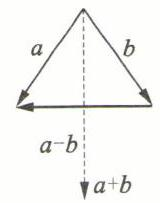
\includegraphics[width=0.2\textwidth]{bodyxb/src/bo_d20cdrf7aajc73bfmvhg_4_1349_1080_160_203_0.jpg}
\end{center}


(第 71 题)

$\therefore {\alpha }_{1} = {\alpha }_{2}$ . 另外,由 $\left( {\vv{a} + \vv{b}}\right)  \cdot  \vv{a} = \left( {\vv{a} + \vv{b}}\right)  \cdot  \vv{b}$ ,也有 $\left( {\vv{a} + \vv{b}}\right)  \cdot  \left( {\vv{a} - \vv{b}}\right)  = 0$ ,可以看出 $\left( {\vv{a} + \vv{b}}\right)  \bot  \left( {\vv{a} - \vv{b}}\right)$ .

72. $- \dfrac{25}{16}$ 提示: $\vv{AP} = \dfrac{1}{4}\vv{AB} + \dfrac{3}{4}\vv{AD},\vv{CP} = \dfrac{1}{4}\vv{CB} + \dfrac{3}{4}\vv{CD} =  - \dfrac{3}{4}\vv{AB} - \dfrac{1}{4}\vv{AD},\vv{AB} \cdot  \vv{AD} = 1$ .

$\vv{AP} \cdot  \vv{CP} =  - \dfrac{1}{16}\left( {\vv{AB} + 3\vv{AD}}\right)  \cdot  \left( {3\vv{AB} + \vv{AD}}\right)  =  - \dfrac{1}{16}\left( {{12} + {10} + 3}\right)  =  - \dfrac{25}{16}.$

73. $\dfrac{28}{29}$ 提示:记 $t = {\mathbf{e}}_{1} \cdot  {\mathbf{e}}_{2}$ ,由 $\left| {2{\mathbf{e}}_{1} - {\mathbf{e}}_{2}}\right|  \leq  \sqrt{2}$ ,可得 $5 - {4t} \leq  2,t \geq  \dfrac{3}{4}$ .

${\left| \vv{a}\right| }^{2} = 2 + {2t},{\left| \vv{b}\right| }^{2} = {10} + {6t},\vv{a} \cdot  \vv{b} = 4 + {4t}$ ,

${\cos }^{2}\theta  = \dfrac{{\left( 4 + 4t\right) }^{2}}{\left( {2 + {2t}}\right) \left( {{10} + {6t}}\right) } = \dfrac{4\left( {1 + t}\right) }{5 + {3t}} = \dfrac{4}{3}\dfrac{3 + {3t}}{5 + {3t}} = \dfrac{4}{3} - \dfrac{8}{3\left( {5 + {3t}}\right) }$ ,在 $t \in  \left\lbrack  {\dfrac{3}{4}, + \infty }\right)$ 上为严格增函数.

当 $t = \dfrac{3}{4}$ 时, ${\cos }^{2}\theta$ 取到最小值 $\dfrac{28}{29}$ .

74. $6 + 2\sqrt{3}$ 提示:由 ${c}^{2} - {2a} \cdot  c - b \cdot  c + 4 = 0$ ,可得 ${\left( c - a - \dfrac{1}{2}b\right) }^{2} = 3$ ,即 $\left| {c - a - \dfrac{1}{2}b}\right|  = \sqrt{3}$ .

$\left( {\mathbf{c} - \vv{a} - \dfrac{1}{2}\vv{b}}\right)  \cdot  \vv{b} = \left| {\mathbf{c} - \vv{a} - \dfrac{1}{2}\vv{b}}\right| \left| \vv{b}\right| \cos \theta  = 2\sqrt{3}\cos \theta$ ,其中 $\theta  = \left\langle  {\mathbf{c} - \vv{a} - \dfrac{1}{2}\vv{b},\vv{b}}\right\rangle$ .

$b \cdot  c = 4 + 2\sqrt{3}\cos \theta$ ,进而 $\left( {a + c}\right)  \cdot  b = 6 + 2\sqrt{3}\cos \theta$ ,所以 $\left( {a + c}\right)  \cdot  b$ 的最大值为 $6 + 2\sqrt{3}$ .

75. $\sqrt{5} : \sqrt{3} : 2$ ,提示:记 $\left| \vv{BC}\right|  = \left| a\right|  = a,\left| \vv{CA}\right|  = \left| b\right|  = b,\left| \vv{AB}\right|  = \left| c\right|  = c$ ,则

$c \cdot  b = \vv{AB} \cdot  \vv{CA} =  - \left| c\right| \left| b\right| \cos A =  - \dfrac{{b}^{2} + {c}^{2} - {a}^{2}}{2} \cdot  b \cdot  a =  - \dfrac{{b}^{2} + {a}^{2} - {c}^{2}}{2} \cdot  a \cdot  c =  - \dfrac{{a}^{2} + {c}^{2} - {b}^{2}}{2}.$

由条件可设 ${b}^{2} + {c}^{2} - {a}^{2} = t,{b}^{2} + {a}^{2} - {c}^{2} = {2t},{c}^{2} + {a}^{2} - {b}^{2} = {3t}$ ,所以

${a}^{2} = \dfrac{5t}{2},{b}^{2} = \dfrac{3t}{2},{c}^{2} = {2t}$ ,所以 $\left| \vv{a}\right|  : \left| \vv{b}\right|  : \left| \mathbf{c}\right|  = a : b : c = \sqrt{5} : \sqrt{3} : 2$ .

76. 4 提示: 设 ${AB}$ 的中点为 $C$ ,则 $5 = \left| {\vv{PA} + \vv{PB}}\right|  = \left| {2\vv{PC}}\right|$ ,所以 $\left| \vv{PC}\right|  = \dfrac{5}{2}$ .

$\vv{PA} \cdot  \vv{PB} = \left( {\vv{PC} + \vv{CA}}\right)  \cdot  \left( {\vv{PC} + \vv{CB}}\right)  = \left( {\vv{PC} - \dfrac{1}{2}\vv{AB}}\right)  \cdot  \left( {\vv{PC} + \dfrac{1}{2}\vv{AB}}\right)  = {\vv{PC}}^{2} - \dfrac{1}{4}{\vv{AB}}^{2} = \dfrac{25}{4} - \dfrac{1}{4}{\vv{AB}}^{2}.$

当 $\left| \vv{AB}\right|$ 取到最小值时,即 ${AB} \bot  m,\vv{PA} \cdot  \vv{PB}$ 最大,最大值为 4 .

77. $\sqrt{3}$ 提示:一方面, $\vv{AO} = \alpha \vv{AE} + \left( {1 - \alpha }\right) \vv{AC} = \dfrac{1}{3}\alpha \vv{AB} + \left( {1 - \alpha }\right) \vv{AC}$ ,

另一方面, $\vv{AO} = k\vv{AD} = \dfrac{1}{2}k\vv{AB} + \dfrac{1}{2}k\vv{AC}$ ,所以 $\dfrac{1}{3}\alpha  = 1 - \alpha  = \dfrac{1}{2}k$ ,可得 $\alpha  = \dfrac{3}{4}$ .

所以 $\vv{AO} = \dfrac{1}{4}\vv{AB} + \dfrac{1}{4}\vv{AC}$ ,又 $\vv{EC} = \vv{EA} + \vv{AC} =  - \dfrac{1}{3}\vv{AB} + \vv{AC}$ .

由 $6\vv{AO} \cdot  \vv{EC} = \dfrac{1}{2}\left( {\vv{AC} + \vv{AB}}\right)  \cdot  \left( {3\vv{AC} - \vv{AB}}\right)  = \vv{AB} \cdot  \vv{AC}$ ,可得 $3{\vv{AC}}^{2} = {\vv{AB}}^{2}$ ,即 $\dfrac{\left| \vv{AB}\right| }{\left| \vv{AC}\right| } = \sqrt{3}$ .

78. $\left\{  {\begin{array}{l} \left( {a + {3b}}\right)  \cdot  \left( {{7a} - {5b}}\right)  = 0, \\  \left( {a - {4b}}\right)  \cdot  \left( {{7a} - {2b}}\right)  = 0 \end{array} \Rightarrow  \left\{  {\begin{array}{l} \left| a\right|  = \left| b\right| , \\  {2a} \cdot  b = {\left| b\right| }^{2} \end{array} \Rightarrow  \cos \theta  = \dfrac{a \cdot  b}{\left| a\right| \left| b\right| } = \dfrac{1}{2} \Rightarrow  \theta  = {60}^{ \circ  }}\right. }\right.$ .

79. (1) ${S}_{\bigtriangleup {ABC}} = \dfrac{1}{2}\left| \vv{AB}\right| \left| \vv{AC}\right|  \cdot  \sin \theta  = 3,\;\therefore \;\left| \vv{AB}\right| \left| \vv{AC}\right|  = \dfrac{6}{\sin \theta }$ . 而 $\vv{AB} \cdot  \vv{AC} = \left| \vv{AB}\right| \left| \vv{AC}\right| \cos \theta  = 6\cot \theta  \in  \left\lbrack  {0,6}\right\rbrack$ ,

$\therefore \;\cot \theta  \in  \left\lbrack  {0,1}\right\rbrack$ ,而 $\theta  \in  \left( {0,\pi }\right) ,\;\therefore \;\theta  \in  \left\lbrack  {\dfrac{\pi }{4},\dfrac{\pi }{2}}\right\rbrack$ .

(2) $f\left( \theta \right)  = 2 \cdot  \dfrac{1 - \cos \left( {{2\theta } + \dfrac{\pi }{2}}\right) }{2} - \sqrt{3}\cos {2\theta } = 1 + \sin {2\theta } - \sqrt{3}\cos {2\theta } = 1 + 2\sin \left( {{2\theta } - \dfrac{\pi }{3}}\right) ,\theta  \in  \left\lbrack  {\dfrac{\pi }{4},\dfrac{\pi }{2}}\right\rbrack$ 时, $\left( {{2\theta } - \dfrac{\pi }{3}}\right)  \in$

$\left\lbrack  {\dfrac{\pi }{6},\dfrac{2}{3}\pi }\right\rbrack  ,\sin \left( {{2\theta } - \dfrac{\pi }{3}}\right)  \in  \left\lbrack  {\dfrac{1}{2},1}\right\rbrack  ,\;\therefore \;f{\left( \theta \right) }_{\max } = 3$ ,此时 $\theta  = \dfrac{5}{12}\pi ,f{\left( \theta \right) }_{\min } = 2$ ,此时 $\theta  = \dfrac{1}{4}\pi$ .

80. 方法一: $\because \vv{AB}\bot \vv{AC},\therefore \vv{AB} \cdot  \vv{AC} = 0,\;\because \vv{AP} =  - \vv{AQ},\vv{BP} = \vv{AP} - \vv{AB},\vv{CQ} = \vv{AQ} - \vv{AC}$ ,

$\therefore \vv{BP} \cdot  \vv{CQ} = \left( {\vv{AP} - \vv{AB}}\right)  \cdot  \left( {\vv{AQ} - \vv{AC}}\right)  = \vv{AP} \cdot  \vv{AQ} - \vv{AP} \cdot  \vv{AC} - \vv{AB} \cdot  \vv{AQ} + \vv{AB} \cdot  \vv{AC}$

$=  - {a}^{2} + \vv{AP} \cdot  \left( {\vv{AB} - \vv{AC}}\right)  =  - {a}^{2} + \dfrac{1}{2}\vv{PQ} \cdot  \vv{BC} =  - {a}^{2} + {a}^{2}\cos \theta .$

$\therefore$ 当 $\theta  = 0$ 时, $\vv{BP} \cdot  \vv{CQ}$ 的值最大,最大值为 0 .

方法二: 把 $A$ 作为原点, $\vv{AB}$ 为 $x$ 轴正方向, $\vv{AC}$ 为 $y$ 轴正方向,建立平面直角坐标系,并设 $P\left( {a\cos \varphi ,a\sin \varphi }\right)$ ,易知 $Q\left( {-a\cos \varphi , - a\sin \varphi }\right)$ . 又设 $B\left( {b,0}\right) ,C\left( {0,c}\right)$ ,依题意 ${b}^{2} + {c}^{2} = {a}^{2},b,c > 0,\vv{BP} = \left( {a\cos \varphi  - b,a\sin \varphi }\right) ,\vv{CQ} = ( - a\cos \varphi$ , $- a\sin \varphi  - c),\;\therefore \;\vv{BP} \cdot  \vv{CQ} =  - {a}^{2}{\cos }^{2}\varphi  + {ab}\cos \varphi  - {a}^{2}{\sin }^{2}\varphi  - {ac}\sin \varphi  =  - {a}^{2} + a\left( {b\cos \varphi  - c\sin \varphi }\right)$ . 其中 $a(b\cos \varphi  -$  $c\sin \varphi ) = b \cdot  \left( {a\cos \varphi }\right)  - c \cdot  \left( {a\sin \varphi }\right)  = \left( {b, - c}\right)  \cdot  \left( {a\cos \varphi ,a\sin \varphi }\right)$ . 向量(b, - c)即为 $\vv{CB}$ ,而 $\left( {a\cos \varphi ,a\sin \varphi }\right)  = \vv{AP}$  $=  - \dfrac{1}{2}\vv{PQ}$ ,

$\therefore a\left( {b\cos \varphi  - c\sin \varphi }\right)  = \vv{CB} \cdot  \vv{AP} =  - \vv{BC} \cdot  \left( {-\dfrac{1}{2}\vv{PQ}}\right)  = \dfrac{1}{2}\vv{PQ} \cdot  \vv{BC} = \dfrac{1}{2} \cdot  \left| \vv{PQ}\right| \left| \vv{BC}\right| \cos \theta  = {a}^{2}\cos \theta$ .

$\therefore \vv{BP} \cdot  \vv{CQ} =  - {a}^{2} + {a}^{2}\cos \theta  =  - {a}^{2}\left( {1 - \cos \theta }\right) ,\theta  \in  \left\lbrack  {0,\pi }\right\rbrack  ,\;\therefore \vv{BP} \cdot  {\vv{CQ}}_{\max } = 0$ ,此时 $\theta  = 0$ .

81. $\vv{AG} \cdot  \vv{BC} = \dfrac{1}{3}\left( {\vv{AB} + \vv{AC}}\right)  \cdot  \left( {\vv{AC} - \vv{AB}}\right)  = \dfrac{1}{3}\left( {{\vv{AC}}^{2} - {\vv{AB}}^{2}}\right)  = 8$ .

由于外心 $O$ 在边 ${AB},{AC}$ 上的射影为中点,所以 $\vv{AO} \cdot  \vv{AB} = \dfrac{1}{2}{\vv{AB}}^{2},\vv{AO} \cdot  \vv{AC} = \dfrac{1}{2}{\vv{AC}}^{2}$ .

所以 $\vv{AO} \cdot  \vv{BC} = \vv{AO} \cdot  \left( {\vv{AC} - \vv{AB}}\right)  = \dfrac{1}{2}\left( {{\vv{AC}}^{2} - {\vv{AB}}^{2}}\right)  = {12}$ .

设内心 $I$ 在边 ${AB},{AC}$ 上的射影分别为 $D,E$ ,则 $\left| \vv{AD}\right|  = \left| \vv{AE}\right|  = \dfrac{5 + 7 - 6}{2} = 3$ ,

所以 $\vv{AI} \cdot  \vv{BC} = \vv{AI} \cdot  \left( {\vv{AC} - \vv{AB}}\right)  = \vv{AI} \cdot  \vv{AC} - \vv{AI} \cdot  \vv{AB} = {21} - {15} = 6$ .

82. $0 = \vv{AG} \cdot  \vv{BG} = \dfrac{1}{3}\left( {\vv{AB} + \vv{AC}}\right)  \cdot  \dfrac{1}{3}\left( {\vv{BC} + \vv{BA}}\right)  = \dfrac{1}{9}\left( {\vv{CB} - 2\vv{CA}}\right)  \cdot  \left( {\vv{CA} - 2\vv{CB}}\right)$ .

记 $\left| \vv{CB}\right|  = a,\left| \vv{CA}\right|  = b$ ,则 $0 = 5\vv{CA} \cdot  \vv{CB} - 2{\vv{CB}}^{2} - 2{\vv{CA}}^{2} = {5ab}\cos C - 2{a}^{2} - 2{b}^{2}$ ,

所以 $\cos C = \dfrac{2{a}^{2} + 2{b}^{2}}{5ab} \geq  \dfrac{4}{5}$ . 当且仅当 $a = b$ 时等号成立,所以 $\cos C$ 的最小值为 $\dfrac{4}{5}$ .

83. 设 $\vv{PB} = \lambda \vv{AB}$ ,则 $f\left( \lambda \right)  = \vv{PB} \cdot  \vv{PC} = \vv{PB} \cdot  \left( {\vv{PB} + \vv{BC}}\right)  = {\vv{AB}}^{2}{\lambda }^{2} + \vv{AB} \cdot  \vv{BC}\lambda$ .

由条件,当 $\lambda  = \dfrac{1}{4}$ 时, $f\left( \lambda \right)$ 最小,所以 $\dfrac{1}{4} =  - \dfrac{\vv{AB} \cdot  \vv{BC}}{2\vv{AB}{}^{2}}$ ,设 $\left| \vv{AB}\right|  = c,\left| \vv{BC}\right|  = a,\left| \vv{AC}\right|  = b$ ,

则 ${c}^{2} = {2ac}\cos B = {a}^{2} + {c}^{2} - {b}^{2}$ ,所以 $b = a,\bigtriangleup {ABC}$ 为等腰三角形.

84. (1) 对任意单位向量 $e,\sqrt{6} \geq  \left| {a \cdot  e}\right|  + \left| {b \cdot  e}\right|  \geq  \left| {a \cdot  e + b \cdot  e}\right|  = \left| {\left( {a + b}\right)  \cdot  e}\right|$ 恒成立,取 $e = \dfrac{a + b}{\left| a + b\right| }$ ,可得 $\sqrt{6} \geq$  $\left| {\vv{a} + \vv{b}}\right|$ ,所以 $6 \geq  1 + 2\vv{a} \cdot  \vv{b} + 4,\vv{a} \cdot  \vv{b} \leq  \dfrac{1}{2}$ .

(2)当 $a \cdot  b = \dfrac{1}{2}$ 时, $\left| {a + b}\right|  = \sqrt{6}$ , $\left| {a - b}\right|  = 2$ ,对任意单位向量 $e$ , $\left| {a \cdot  e}\right|  + \left| {b \cdot  e}\right|  = \max \{ \left| {\left( {a + b}\right)  \cdot  e}\right|$ ,

$\left| {\left( {a - b}\right)  \cdot  e}\right| \}  \leq  \max \{ \left| \left( {a + b}\right) \right| ,\left| \left( {a - b}\right) \right| \}  = \sqrt{6}$ 恒成立,由 (1) (2) 可知 $a \cdot  b$ 的最大值为 $\dfrac{1}{2}$ .

85. 记 ${\mathbf{S}}_{n} = {\vv{a}}_{1} + {\vv{a}}_{2} + \cdots  + {\vv{a}}_{n}$ ,由条件对 $i = 1,2,\cdots ,n,\left| {{\mathbf{S}}_{n} - {\vv{a}}_{i}}\right|  \leq  \left| {\vv{a}}_{i}\right|$ ,

两边平方,可得 ${\left| {\mathbf{S}}_{n} - {\vv{a}}_{i}\right| }^{2} \leq  {\left| {\vv{a}}_{i}\right| }^{2}$ ,即 ${\mathbf{S}}_{n}{}^{2} \leq  2{\mathbf{S}}_{n} \cdot  {\vv{a}}_{i}$ ,

两边对 $i$ 求和,得 $n{\mathbf{S}}_{n}{}^{2} \leq  2{\mathbf{S}}_{n}{}^{2}$ ,即 $\left( {n - 2}\right) {\mathbf{S}}_{n}{}^{2} \leq  0$ .

因为 $n > 2$ ,所以 ${\mathbf{S}}_{n}{}^{2} \leq  0,{\mathbf{S}}_{n} = \mathbf{0}$ .

86. 记 $A = {A}_{6}$ ,向量 $\vv{{A}_{i}{A}_{i + 1}} = {a}_{i}\left( {i = 1,2,3,4,5}\right) ,a = {a}_{1} + {a}_{2} + \cdots  + {a}_{5}$ .

向量 ${\vv{b}}_{ij} = {\vv{a}}_{i} + {\vv{a}}_{j}\left( {1 \leq  i < j \leq  5}\right)$ ,则 $\mathop{\sum }\limits_{{1 \leq  i < j \leq  5}}{\vv{b}}_{ij} = {\vv{b}}_{12} + {\vv{b}}_{13} + \cdots  = 4\vv{a}$ (1)

由条件,对任意 $1 \leq  i < j \leq  5,\left| {a - {b}_{ij}}\right|  = \left| {b}_{ij}\right|$ ,两边平方得 ${a}^{2} = {2a} \cdot  {b}_{ij}$ .

两边对 $i,j$ 求和,得 ${10}{a}^{2} = \mathop{\sum }\limits_{{1 \leq  i < j \leq  5}}{2a} \cdot  {b}_{ij} = {2a} \cdot  \mathop{\sum }\limits_{{1 \leq  i < j \leq  5}}{b}_{ij} = {2a} \cdot  {4a} = 8{a}^{2}$ ,

所以 $\vv{a} = \mathbf{0}$ ,即 $\vv{{A}_{1}{A}_{2}} + \vv{{A}_{2}{A}_{3}} + \vv{{A}_{3}{A}_{4}} + \vv{{A}_{4}{A}_{5}} + \vv{{A}_{5}A} = \mathbf{0}$ ,所以点 $A$ 与点 ${A}_{1}$ 重合.

87. C 提示: 几何上,由于 ${OA}$ 与 ${OB}$ 并不一定相等,故选项 $A$ 不一定成立,反例: $m = n$ 时, $\vv{OP} = {ma} + {nb} = m\left( {a + b}\right)$ ,具体地: $\cos \angle {POA} = \dfrac{\vv{OP} \cdot  \vv{OA}}{\left| \vv{OP}\right| \left| \vv{OA}\right| } = \dfrac{m\left( {{a}^{2} + a \cdot  b}\right) }{\left| \vv{OP}\right|  \cdot  \left| a\right| }$ , $\cos \angle {POB} = \dfrac{\vv{OP} \cdot  \vv{OB}}{\left| \vv{OP}\right| \left| \vv{OB}\right| } = \dfrac{m\left( {{b}^{2} + a \cdot  b}\right) }{\left| \vv{OP}\right|  \cdot  \left| b\right| }$ . 若 $\angle {POA} = \angle {POB}$ ,则 $\dfrac{{a}^{2} + a \cdot  b}{\left| a\right| } = \dfrac{{b}^{2} + a \cdot  b}{\left| b\right| }$ . 又 $a \cdot  b = \left| a\right|  \cdot  \left| b\right| \cos \angle {AOB}$ ,整理得 $\left( {\left| a\right|  - \left| b\right| }\right) \left( {1 - \cos \angle {AOB}}\right)  = 0.\angle {AOB} \in  \left( {0,\pi }\right)$ ,

$\therefore 1 - \cos \angle {AOB} \neq  0,\therefore \angle {POA} = \angle {POB} \Rightarrow  \left| a\right|  = \left| b\right|$ ,但题目中并未说明 $\left| a\right|$ 一定等于 $\left| b\right|$ ,故点 $P$ 不一定在 $\angle {AOB}$ 的平分线所在的直线上. 对于选项 $B : m =  - n$ 时, $\vv{OP} = {ma} + {nb} = n\left( {b - a}\right)  = n\vv{AB}$ ,可见 $\vv{OP}//\vv{AB}$ ,但 $\vv{OP}$ 的起点是 $O$ ,故点 $P$ 并不在直线 ${AB}$ 上,选项 $B$ 错误. 对于选项 $C : m = 0$ 时, $\vv{OP} = {nb} = n\vv{OB},\vv{OP}//\vv{OB}$ 且有公共点 $O$ ,故点 $P$ 在直线 ${OB}$ 上,选项 $C$ 正确. 对于选项 $D : m \neq  0$ 时,若点 $P$ 在边 ${OA}$ 所在的直线上,应存在 $\lambda$ ,使得 $\vv{OP} = \lambda \vv{OA}$ ,

$\therefore {ma} + {nb} = {\lambda a},\therefore \left( {m - \lambda }\right) a + {nb} = 0.a,b$ 不共线, $\therefore \left\{  \begin{array}{l} m - \lambda  = 0, \\  n = 0. \end{array}\right.$ 即 $\left\{  \begin{array}{l} \lambda  = m, \\  n = 0, \end{array}\right.$ 然而 $n = 0$ 并不一定成立,故选项 D 错误. 综上, 选 C.

88. D 提示: $\because \vv{CD} = 2\vv{DB},\therefore \vv{DB} = \dfrac{1}{2}\vv{CD},\vv{CB} = \vv{CD} + \vv{DB} = \dfrac{3}{2}\vv{CD},\therefore \vv{CD} = \dfrac{2}{3}\vv{CB} = \dfrac{2}{3}\left( {\vv{AB} - \vv{AC}}\right)  = r\vv{AB} +$  $s\vv{AC}.\because \vv{AB},\vv{AC}$ 不共线, $\therefore r = \dfrac{2}{3},s =  - \dfrac{2}{3},r + s = 0$ .

89. A 提示: 由于 $\left| \dfrac{a}{\left| a\right| }\right|  = \left| \dfrac{b}{\left| b\right| }\right|  = 1$ ,不难看出 $\dfrac{a}{\left| a\right| }$ 和 $\dfrac{b}{\left| b\right| }$ 为两边的平行四边形是一个菱形,此时,点 $P$ 应在 $\angle {AOB}$ 的平分线所在的直线上. 证明如下: $t \neq  0$ 时, $\cos \angle {AOP} = \dfrac{\vv{OA} \cdot  \vv{OP}}{\left| \vv{OA}\right|  \cdot  \left| \vv{OP}\right| } = \dfrac{t\left( {\dfrac{{a}^{2}}{\left| a\right| } + \dfrac{a \cdot  b}{\left| b\right| }}\right) }{\left| a\right|  \cdot  \left| p\right| } = \dfrac{t}{\left| p\right| } \cdot  \left( {1 + \dfrac{a \cdot  b}{\left| a\right| \left| b\right| }}\right) ,\cos \angle {BOP} =$  $\dfrac{\vv{OB} \cdot  \vv{OP}}{\left| \vv{OB}\right|  \cdot  \left| \vv{OP}\right| } = \dfrac{t\left( {\dfrac{{b}^{2}}{\left| b\right| } + \dfrac{a \cdot  b}{\left| a\right| }}\right) }{\left| b\right|  \cdot  \left| p\right| } = \dfrac{t}{\left| p\right| } \cdot  \left( {1 + \dfrac{a \cdot  b}{\left| a\right|  \cdot  \left| b\right| }}\right) .$

$\therefore \cos \angle {AOP} = \cos \angle {BOP}$ ,又 $\angle {AOP}$ , $\angle {BOP} \in  \left( {0,\pi }\right)$ , $\therefore \angle {AOP} = \angle {BOP}$ ,而 $t = 0$ 时 $\vv{OP} = p = 0$ , $P$ 点即 $O$ 点.

$\therefore$ 点 $P$ 总在 $\angle {AOB}$ 的平分线所在的直线上,选项 $A$ 正确,选项 $C$ 不一定正确,因为 $t$ 的值不确定,选项 $B,D$ 不一定正确, 因为角平分线与垂直平分线或中线重合是有条件的. 综上, 选 A.

90. D 提示: 由对称性,考虑 $\lambda ,\mu  \geq  0$ ,此时点 $P$ 所在的区域为 $\bigtriangleup {AOB}$ 及其内部,面积为 $\sqrt{3}$ ,进而得所求面积为 $4\sqrt{3}$ .

91. $- \dfrac{4}{3}$ 提示: $2{e}_{1} + 3{e}_{2}$ 与 $k{e}_{1} - 2{e}_{2}$ 共线, $\therefore$ 存在 $\lambda$ ,使 $2{e}_{1} + 3{e}_{2} = \lambda \left( {k{e}_{1} - 2{e}_{2}}\right) .\;\because {e}_{1},{e}_{2}$ 不共线, $\therefore$

$\left\{  {\begin{array}{l} 2 = {\lambda k}, \\  3 =  - {2\lambda }, \end{array}\text{ 解得 }\left\{  \begin{array}{l} \lambda  =  - \dfrac{3}{2}, \\  k =  - \dfrac{4}{3}. \end{array}\right. }\right.$

92. ①②④ 提示:两个向量不平行是可以作为基底的充要条件.

93. $- \dfrac{2}{3}a + \dfrac{1}{3}b$ 提示: $\vv{DE} = \vv{CE} - \vv{CD}$ ,其中 $\vv{CD} = \vv{BD} - \vv{BC} =  - \dfrac{2}{3}\vv{BC} =  - \dfrac{2}{3}\left( {\vv{AC} - \vv{AB}}\right)  =  - \dfrac{2}{3}\left( {b - a}\right)$ ,

$\therefore \vv{DE} = \vv{CE} - \vv{CD} = \dfrac{1}{3}\vv{CA} - \vv{CD} =  - \dfrac{1}{3}\vv{AC} - \vv{CD} =  - \dfrac{1}{3}b + \dfrac{2}{3}\left( {b - a}\right)  = \dfrac{1}{3}b - \dfrac{2}{3}a$ .

94. $\lambda  \neq  4$ 提示:由题意, $m,n$ 不共线. $\because m,n$ 共线 $\Leftrightarrow$ 存在唯一的 $\mu$ ,使得 $m = {\mu n}\therefore m,n$ 不共线 $\Leftrightarrow$ 对 $\forall \mu  \in  \mathbf{R}$ ,都有 $m$  $\neq  {\mu n}$ ,即 $\forall \mu  \in  \mathbf{R},\left( {a + {2b}}\right)  - \mu \left( {{2a} + {\lambda b}}\right)  \neq  0$ ,即 $\left( {1 - {2\mu }}\right) a + \left( {2 - {\mu \lambda }}\right) b \neq  0.\;\because a,b$ 不共线, $\therefore 1 - {2\mu } \neq  0$ 时, $m - {\mu n}$  $\neq  0$ 总成立; 当 $1 - {2\mu } = 0$ 时, $2 - {\mu \lambda } \neq  0$ ,即 $2 - \dfrac{1}{2}\lambda  \neq  0,\lambda  \neq  4$ ,

$\therefore \lambda  \neq  4$ 时,对 $\forall \mu  \in  \mathbf{R}$ 都有 $m \neq  {\mu n}$ .

95. ①②④ 提示:根据向量的运算法则,命题①,②正确. 对于命题③: ${pa} = {pb} \Leftrightarrow  p\left( {a - b}\right)  = 0 \Leftrightarrow  p = 0$ 或 $a = b,\therefore$ 命题③ 不成立. 对于命题④, ${pa} = {qa} \Leftrightarrow  \left( {p - q}\right) a = 0.\;\because \;a \neq  0,\;\therefore \;p - q = 0 \Leftrightarrow  p = q.$

$\therefore$ 命题④成立. 综上,真命题是①②④.

96. $\dfrac{\dfrac{a}{\left| a\right| } + \dfrac{b}{\left| b\right| }}{\left| \dfrac{a}{\left| a\right| } + \dfrac{b}{\left| b\right| }\right| }$ 提示: 向量 $c$ 与 $\dfrac{a}{\left| a\right| } + \dfrac{b}{\left| b\right| }$ 的方向相同,所以 $c = \dfrac{\dfrac{a}{\left| a\right| } + \dfrac{b}{\left| b\right| }}{\dfrac{a}{\left| a\right| } + \dfrac{b}{\left| b\right| }}$ .

97. 3 提示:过点 $C$ 作 ${OB}$ 的平行线,交 ${OA}$ 于点 $D$ ,则 $\vv{OD} = m\vv{OA},\vv{DC} = n\vv{OB}$ ,由 $\left| \vv{OA}\right|  = \left| \vv{OB}\right|  = 1$ 可知 $m = \left| \vv{OD}\right| ,n =$  $\left| \vv{DC}\right|$ . 在 $\bigtriangleup {ODC}$ 中,由正弦定理得 $\dfrac{\left| \vv{OD}\right| }{\sin {45}^{ \circ  }} = \dfrac{\left| \vv{DC}\right| }{\sin \alpha } = \dfrac{\left| \vv{OC}\right| }{\sin \left( {\alpha  + {45}^{ \circ  }}\right) }$ .

由条件得 $\sin \alpha  = \dfrac{7\sqrt{2}}{10},\sin \left( {\alpha  + {45}^{ \circ  }}\right)  = \dfrac{4}{5}$ ,所以 $\underset{\dfrac{7}{2}}{\underbrace{\dfrac{m}{\sqrt{2}}}} = \dfrac{n}{\dfrac{7\sqrt{2}}{10}} = \dfrac{\sqrt{2}}{\dfrac{4}{5}},m = \dfrac{5}{4},n = \dfrac{7}{4},m + n = 3$ .

98. $\because \dfrac{CD}{AB} = k,\;\therefore \vv{DC} = k\vv{AB} = {kb},\vv{BC} = \vv{BA} + \vv{AD} + \vv{DC} =  - b + a + {kb} = a + \left( {k - 1}\right) b,\vv{MN} = \vv{MA} + \vv{AB} + \vv{BN} =$  $- \dfrac{1}{2}\vv{AD} + \vv{AB} + \dfrac{1}{2}\vv{BC} =  - \dfrac{1}{2}\vv{a} + \vv{b} + \dfrac{1}{2}\vv{a} + \dfrac{1}{2}\left( {k - 1}\right) \vv{b} = \dfrac{1}{2}\left( {k + 1}\right) \vv{b}.$

注意: $\vv{MN}$ 也可由 $\vv{MN} = \dfrac{1}{2}\left( {\vv{AB} + \vv{DC}}\right)$ 得到.

99. 由题意, $\vv{AB} + \vv{BC} = \vv{AC} = a,\vv{BD} = \vv{BC} + \vv{CD} = \vv{BC} + \vv{BA} =  - \vv{AB} + \vv{BC} = b.\left\{  \begin{array}{l} \vv{AB} + \vv{BC} = a, \\   - \vv{AB} + \vv{BC} = b, \end{array}\right.$

$\therefore \left\{  \begin{array}{l} \vv{AB} = \dfrac{a - b}{2}, \\  \vv{BC} = \dfrac{a + b}{2}. \end{array}\right.$

100. 记 $\vv{AB} = c,\vv{AC} = b$ ,则 $\vv{BC} = \vv{AC} - \vv{AB} = b - c$ . 思路是在 $B,P,N$ 共线 (或 $C,P,M$ 共线也可) 上寻找关系. $\vv{BP} = \vv{BC} + \vv{CP}$ ,设 $\vv{CP} = \mu \vv{CM}$ ,

\begin{center}
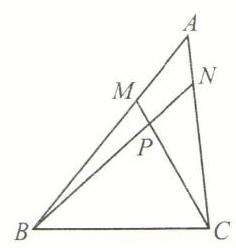
\includegraphics[width=0.2\textwidth]{bodyxb/src/bo_d20cdrf7aajc73bfmvhg_7_1206_1565_236_248_0.jpg}
\end{center}


(第 100 题)

$\therefore \vv{BP} = \vv{BC} + \vv{CP} = \vv{BC} + \mu \vv{CM} = \vv{BC} + \mu \left( {\vv{AM} - \vv{AC}}\right)  = b - c + \mu \left( {\dfrac{1}{3}c - b}\right)  = \left( {1 - \mu }\right) b +$  $\left( {\dfrac{1}{3}\mu  - 1}\right) \mathbf{c},\vv{BN} = \vv{BC} + \vv{CN} = \vv{BC} + \dfrac{3}{4}\vv{CA} = \vv{b} - \mathbf{c} - \dfrac{3}{4}\vv{b} = \dfrac{1}{4}\vv{b} - \mathbf{c}.\;\because B,P,N$ 共线,

$\therefore$ 存在 $\lambda$ ,使得 $\vv{BP} = \lambda \vv{BN},\therefore \left( {1 - \mu }\right) b + \left( {\dfrac{1}{3}\mu  - 1}\right) c = \dfrac{1}{4}{\lambda b} - {\lambda c}.\because b,c$ 不共线,

$\therefore \left\{  \begin{array}{l} 1 - \mu  = \dfrac{1}{4}\lambda , \\  \dfrac{1}{3}\mu  - 1 =  - \lambda , \end{array}\right.$ 解得 $\left\{  \begin{array}{l} \lambda  = \dfrac{8}{11}, \\  \mu  = \dfrac{9}{11}. \end{array}\right.$ 而 $\vv{AP} = \vv{AB} + \vv{BP} = \mathbf{c} + \left( {1 - \mu }\right) \vv{b} + \left( {\dfrac{1}{3}\mu  - 1}\right) \mathbf{c} = \left( {1 - \mu }\right) \vv{b} + \dfrac{1}{3}\mu \mathbf{c} = \dfrac{2}{11}\vv{b} + \dfrac{3}{11}\mathbf{c} =$  $\dfrac{3}{11}\vv{AB} + \dfrac{2}{11}\vv{AC}$ . 证毕.

101. $\vv{AG} = \dfrac{1}{3}\vv{AB} + \dfrac{1}{3}\vv{AC} = \dfrac{1}{3x}\vv{AM} + \dfrac{1}{3y}\vv{AN}$ ,由 $M,G,N$ 三点共线可知 $\dfrac{1}{3x} + \dfrac{1}{3y} = 1$ ,所以 $\dfrac{xy}{x + y} = \dfrac{1}{3}$ .

102. 证明: 由于 $\vv{OA},\vv{OB},\vv{OC}$ 不都平行,则 $\vv{OP}$ 必可表示为其中 2 个的线性组合,另一个取系数为 0 . , $\vv{OP}$ 可表示为

$\vv{OA},\vv{OB},\vv{OC}$ 三者线性组合. 下面考察 $x + y + z = 1$ 组合的存在情况.

①若 $\vv{CP}//\vv{BA}$ ,则 $\vv{CP} = x\vv{BA},x \in  \mathbf{R}$ 且唯一, $\therefore  - \vv{OC} + \vv{OP} = x\left( {-\vv{OB} + \vv{OA}}\right) ,\vv{OP} = x \cdot  \vv{OA} - x \cdot  \vv{OB} + \vv{OC}$ . 令 $y =$  $- x,z = 1$ ,满足 $x + y + z = 1$ .

②若 $\vv{CP} \times  \vv{BA}$ ,设直线 ${CP}$ 交直线 ${AB}$ 于点 $D.\because C,P,D$ 共线, $\therefore \vv{OP} = z\vv{OC} + \left( {1 - z}\right) \vv{OD}$ . 又 $A,D,B$ 共线,

$\therefore \vv{OD} = t\vv{OA} + \left( {1 - t}\right) \vv{OB}.\;\therefore \vv{OP} = \left( {1 - z}\right) t\vv{OA} + \left( {1 - z}\right) \left( {1 - t}\right) \vv{OB} + z\vv{OC}$ . 令 $x = \left( {1 - z}\right) t,y = \left( {1 - z}\right) \left( {1 - t}\right)$ ,满足 $x + y + z = 1,\;\therefore \;$ 存在.

下证唯一. 假设 ${x}^{\prime },{y}^{\prime },{z}^{\prime }$ 也满足,则 $x\vv{OA} + y\vv{OB} + z\vv{OC} = {x}^{\prime }\vv{OA} + {y}^{\prime }\vv{OB} + {z}^{\prime }\vv{OC},x + y + z = {x}^{\prime } + {y}^{\prime } + {z}^{\prime } = 1$ .

$\therefore \left( {x - {x}^{\prime }}\right) \vv{OA} + \left( {y - {y}^{\prime }}\right) \vv{OB} + \left( {z - {z}^{\prime }}\right) \vv{OC} = \mathbf{0}$

记 $a = x - {x}^{\prime },b = y - {y}^{\prime },c = z - {z}^{\prime }$ ,则 $a + b + c = 0,\;\therefore \;a \cdot  \vv{OA} + b \cdot  \vv{OB} + \left( {-a - b}\right) \vv{OC} = \mathbf{0}$ .

$a\left( {\vv{OA} - \vv{OC}}\right)  + b\left( {\vv{OB} - \vv{OC}}\right)  = 0,\;\therefore \;a \cdot  \vv{CA} + b \cdot  \vv{CB} = 0.\;\because \;\vv{CA} \times  \vv{CB},\;\therefore \;a = b = 0$ ,即 $\left\{  \begin{array}{l} x = {x}^{\prime }, \\  y = {y}^{\prime }. \end{array}\right.$

$\therefore z = 1 - x - y = 1 - {x}^{\prime } - {y}^{\prime } = {z}^{\prime }$ ,矛盾! 得证.

103. A 提示: $x\left( {\vv{a} + \vv{b}}\right)  + y\left( {\vv{a} - \vv{b}}\right)  = \left( {x + y}\right) \vv{a} + \left( {x - y}\right) \vv{b} = 2\vv{a} + 4\vv{b}.\;\because \vv{a},\vv{b}$ 不共线, $\;\therefore \;\left\{  \begin{array}{l} x + y = 2, \\  x - y = 4, \end{array}\right.$ 解得 $\left\{  \begin{array}{l} x = 3, \\  y =  - 1. \end{array}\right.$

104. D 提示: $\because {\mathbf{e}}_{1}$ 与 ${\mathbf{e}}_{2}$ 不共线,故由 $\vv{a} = \vv{b}$ 可得 $\left\{  \begin{array}{l} {2\lambda } = 3{\lambda }^{2} - 1, \\  1 = 6 - {5\lambda }, \end{array}\right.$ 解得 $\lambda  = 1$ .

105. B 提示: 由题意: $\cos \angle {AOC} = \dfrac{\vv{OC} \cdot  \vv{OA}}{\left| \vv{OC}\right| \left| \vv{OA}\right| },\vv{OC} \cdot  \vv{OA} = \left( {m\vv{OA} + n\vv{OB}}\right)  \cdot  \vv{OA} = m{\vv{OA}}^{2} + 0 = m,{\left| \vv{OC}\right| }^{2} = {\vv{OC}}^{2} = {m}^{2}{\vv{OA}}^{2} +$  ${n}^{2}{\vv{OB}}^{2} + {2mn}\vv{OA} \cdot  \vv{OB} = {m}^{2} + 3{n}^{2},\;\therefore \;\left| \vv{OC}\right|  = \sqrt{{m}^{2} + 3{n}^{2}}.\;\therefore \;\cos \angle {AOC} = \cos {30}^{ \circ  } = \dfrac{\sqrt{3}}{2} = \dfrac{m}{\sqrt{{m}^{2} + 3{n}^{2}}}$ , $\therefore \dfrac{{m}^{2} + 3{n}^{2}}{{m}^{2}} = \dfrac{4}{3},\;\therefore \dfrac{{m}^{2}}{{n}^{2}} = 9,\dfrac{m}{n} = 3$ (-3 舍去,因点 $C$ 在 $\angle {AOB}$ 内).

106. A 提示: $\vv{OD} = \vv{OA} + \vv{AD} = \vv{OA} + \vv{AC} + \vv{CD}$ ,其中 $\vv{AC} = \dfrac{1}{3}\vv{AB}$ , $\vv{CD} = \dfrac{1}{3}\vv{CB} = \dfrac{1}{3} \cdot  \dfrac{2}{3}\vv{AB} = \dfrac{2}{9}\vv{AB}$ , $\vv{AB} = \vv{OB} - \vv{OA} = b -$  $\vv{a},\;\therefore \;\vv{OD} = \vv{OA} + \vv{AC} + \vv{CD} = \vv{OA} + \dfrac{5}{9}\vv{AB} = \vv{a} + \dfrac{5}{9}\left( {\vv{b} - \vv{a}}\right)  = \dfrac{1}{9}\left( {4\vv{a} + 5\vv{b}}\right) .$

107. B 提示: 取 $c = a - b$ ,①正确; 由 $b$ 与 $c$ 不平行,结合平面向量基本定理,②正确; 取单位向量 $a$ 与 $b$ 的夹角为 ${60}^{ \circ  }$ ,则对任意 $\lambda ,{\left| a - \lambda b\right| }^{2} = {\lambda }^{2} - \lambda  + 1 = {\left( \lambda  - \dfrac{1}{2}\right) }^{2} + \dfrac{3}{4}$ ,取 $\mu  = \dfrac{1}{2}$ ,可知对任意单位向量 $c$ 和实数 $\lambda ,\left| {\mu c}\right|  < \left| {a - {\lambda b}}\right|$ ,③不正确; 取向量 $\vv{a}$ 满足: $\left| \vv{a}\right|  = \left| \lambda \right|  + \left| \mu \right|  + 1 > \left| \lambda \right|  + \left| \mu \right|$ ,则对任意单位向量 $\vv{b}$ 与 $\mathbf{c}$ ,均有 $\left| \vv{a}\right|  > \left| {\lambda \vv{b}}\right|  + \left| {\mu \mathbf{c}}\right|  \geq$  $\left| {\lambda \vv{b} + \mu \mathbf{c}}\right|$ ,④不正确

108. ①④ 提示:对于①,由于 $a$ , $b$ 共线,且 $\left| a\right|  = \left| b\right|$ ,可知 $a = b$ 或 $a =  - b$ ,故(a - b)与 $\left( {a + b}\right)$ 中必有一个是零向量,而零向量与任意向量平行,故 $\left( {\vv{a} - \vv{b}}\right) //\left( {\vv{a} + \vv{b}}\right)$ 正确.

对于②, $a = {2e} = 2\left( {\dfrac{1}{3}b}\right)  = \dfrac{2}{3}b$ ,故②错误.

对于③, $\because {e}_{1} \neq  {e}_{2}\;\therefore {e}_{1} - {e}_{2} \neq  0,\;\therefore \;\left| {{e}_{1} - {e}_{2}}\right|  \neq  0.\left| a\right|  = \left| {{e}_{1} - {e}_{2}}\right| ,\left| b\right|  = \left| {-3\left( {{e}_{1} - {e}_{2}}\right) }\right|  = 3\left| {{e}_{1} - {e}_{2}}\right|$ ,

$\therefore \left| \vv{a}\right|  = \dfrac{1}{3}\left| \vv{b}\right|$ ,故③ 错误.

对于④ $\vv{BD} = \vv{DC}$ ,而 $\vv{BD} = \vv{AD} - \vv{AB},\vv{DC} = \vv{AC} - \vv{AD},\therefore \vv{AD} - \vv{AB} = \vv{AC} - \vv{AD},\therefore \vv{AB} + \vv{AC} = 2\vv{AD}$ ,故④正确. 综上, 真命题是①④.

109. $1 + \dfrac{\sqrt{3}}{2},\dfrac{\sqrt{3}}{2}$ 提示: 设 $\left| \vv{AB}\right|  = 1$ ,则 $\left| \vv{BC}\right|  = \left| \vv{DE}\right|  = \sqrt{2},\left| \vv{DB}\right|  = \dfrac{\sqrt{6}}{2}$ ,过点 $D$ 作 ${DF} \bot  {AB}$ 于点 $F$ ,则 $\vv{AF} = x\vv{AB},\vv{FD}$  $= y\vv{AC}$ . 由 $\left| \vv{AB}\right|  = \left| \vv{AC}\right|  = 1$ ,可知 $x = \left| \vv{AF}\right| ,y = \left| \vv{FD}\right|$ ,在直角三角形 ${BFD}$ 中, $\left| \vv{DB}\right|  = \dfrac{\sqrt{6}}{2},\angle {DBF} = {45}^{ \circ  }$ ,所以 $\left| \vv{BF}\right|  = \left| \vv{FD}\right|  = \dfrac{\sqrt{3}}{2},x = 1 + \dfrac{\sqrt{3}}{2},y = \dfrac{\sqrt{3}}{2}$ .

110. $\dfrac{5}{8},\dfrac{5}{16}$ 提示:如图,设 ${AI}$ 延长线交 ${BC}$ 于点 $M$ , $\because {AB} = {AC}$ ,且 $I$ 是内心 $\;\therefore {AM}$ 垂直平分线段 ${BC},\therefore {BM} = {MC} = \dfrac{1}{2}{BC} = 3,\because {AB} = 5,{AM} \bot  {BC},\therefore {AM} = 4$ . 记 ${AI} = r$ ,有 ${S}_{\bigtriangleup {ABC}} = \dfrac{1}{2} \cdot  r \cdot  \left( {{AB} + {BC} + {CA}}\right)  = \dfrac{1}{2}{BC} \cdot  {AM}$ ,

\begin{center}
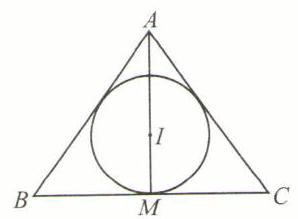
\includegraphics[width=0.2\textwidth]{bodyxb/src/bo_d20cdrf7aajc73bfmvhg_8_1236_1906_298_219_0.jpg}
\end{center}


(第 110 题)

$\therefore \;r = \dfrac{{BC} \cdot  {AM}}{{AB} + {BC} + {CA}} = \dfrac{6 \times  4}{5 + 6 + 5} = \dfrac{3}{2}$ .

$\therefore \vv{AI} = \dfrac{{AM} - r}{AM} \cdot  \vv{AM} = \dfrac{4 - \dfrac{3}{2}}{4}\vv{AM} = \dfrac{5}{8}\vv{AM},\vv{AM} = \vv{AB} + \dfrac{1}{2}\vv{BC}$ ,

$\therefore \vv{AI} = \dfrac{5}{8}\vv{AB} + \dfrac{5}{16}\vv{BC}$ ,即 $\left( {x,y}\right)  = \left( {\dfrac{5}{8},\dfrac{5}{16}}\right)$ .

111. $\left( {-\infty ,0}\right) ,\left( {\dfrac{1}{2},\dfrac{3}{2}}\right)$ 提示: 由题意, $\vv{OB}$ 与 $\vv{AB}$ (或 $\vv{OM}$ )是平面内不共线的两个向量 (否则由 ${OM}//{AB}$ 将有 $A,B,O,M$ 四点共线) $\therefore$ 存在唯一的 $\left( {{\lambda }_{1},{\lambda }_{2}}\right)$ ,使得 $\vv{OP} = {\lambda }_{1}\vv{OB} + {\lambda }_{2}\vv{AB}$ . 根据题意, ${\lambda }_{1},{\lambda }_{2}$ 应满足 $\left\{  \begin{array}{l} 0 < {\lambda }_{1} < 1, \\  {\lambda }_{2} > 0. \end{array}\right.$ 所以 $\vv{OP} = {\lambda }_{1}\vv{OB} +$  ${\lambda }_{2}\vv{AB} = {\lambda }_{1}\vv{OB} + {\lambda }_{2}\left( {\vv{OB} - \vv{OA}}\right)  =  - {\lambda }_{2}\vv{OA} + \left( {{\lambda }_{1} + {\lambda }_{2}}\right) \vv{OB} = x\vv{OA} + y\vv{OB}.\because \vv{OA},\vv{OB}$ 不共线 (否则 $A,B,O,M$ 四点将共线), $\therefore \left\{  \begin{array}{l} x =  - {\lambda }_{2}, \\  y = {\lambda }_{1} + {\lambda }_{2}, \end{array}\right.$ 即 $\left\{  \begin{array}{l} {\lambda }_{1} = x + y, \\  {\lambda }_{2} =  - x. \end{array}\right.$ 由 ${\lambda }_{2} > 0$ 知: $- x > 0,x < 0$ ,即 $x \in  \left( {-\infty ,0}\right)$ ; 当 $x =  - \dfrac{1}{2}$ 时, ${\lambda }_{1} = y - \dfrac{1}{2}$ ,由 0 $< {\lambda }_{1} < 1$ 知, $\dfrac{1}{2} < y < \dfrac{3}{2}$ ,即 $y \in  \left( {\dfrac{1}{2},\dfrac{3}{2}}\right)$ .

112. 5,5 提示: $\vv{a} \cdot  \vv{b} = \left| \vv{a}\right|  \cdot  \left| \vv{b}\right|  \cdot  \cos \angle {AOB} =  - \dfrac{1}{2},{\left| \vv{a} + \vv{b}\right| }^{2} = {\left( \vv{a} + \vv{b}\right) }^{2} = {\left| \vv{a}\right| }^{2} + {\left| \vv{b}\right| }^{2} + 2\vv{a} \cdot  \vv{b} = 1 + 1 - 1 = 1$ .

$\therefore \left| {a + b}\right|  = 1.\;\because \vv{OC} \cdot  \vv{OA} = \left| \vv{OC}\right|  \cdot  \left| \vv{OA}\right|  \cdot  \cos \angle {COA} = \left| \vv{OC}\right|  \cdot  \left| \vv{OB}\right|  \cdot  \cos \angle {COB} = \vv{OC} \cdot  \vv{OB}$ .

$\therefore \left( {{\lambda a} + {\mu b}}\right)  \cdot  a = \left( {{\lambda a} + {\mu b}}\right)  \cdot  b$ ,即 $\lambda \left( {{a}^{2} - a \cdot  b}\right)  = \mu \left( {{b}^{2} - a \cdot  b}\right)$ ,而 ${a}^{2} - a \cdot  b = {b}^{2} - a \cdot  b \neq  0.\;\therefore \lambda  = \mu$ .

$\therefore \left| \vv{OC}\right|  = \left| \lambda \right| \left| {a + b}\right|  = \left| \lambda \right|  = 5$ . $\;\therefore \lambda  = \mu  =  \pm  5$ . 由于 ${OC}$ 平分的 $\angle {AOB} = {120}^{ \circ  } < {180}^{ \circ  }$ ,故取 $\lambda  = \mu  = 5$ .

113. 1 提示: 根据题意, $O$ 和 $H$ 分别是 $\bigtriangleup {ABC}$ 的外心和垂心.

\begin{center}
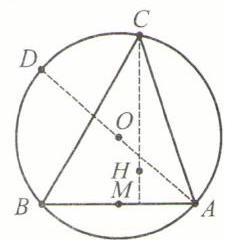
\includegraphics[width=0.2\textwidth]{bodyxb/src/bo_d20cdrf7aajc73bfmvhg_9_1208_925_225_240_0.jpg}
\end{center}


(第 113 题)

情况 (1), $\bigtriangleup {ABC}$ 为直角三角形. 不失一般性,假定此时 $\angle A = {90}^{ \circ  }$ ,则 $O$ 为 ${BC}$ 边的中点,而点 $H$ 与顶点 $A$ 重合. $\vv{OH} = \vv{OA},\vv{OA} + \vv{OB} + \vv{OC} = \vv{OA},\therefore m = 1$ . 情况 (2), $\bigtriangleup {ABC}$ 不是直角三角形.

$\because O$ 为 $\bigtriangleup {ABC}$ 的外心, $\therefore \left| \vv{OA}\right|  = \left| \vv{OB}\right|  = \left| \vv{OC}\right| ,\;\therefore \;\vv{O{A}^{2}} = {\vv{OB}}^{2} = {\vv{OC}}^{2}$ . 在 ${\vv{OA}}^{2} = {\vv{OB}}^{2}$ 中,有 $\vv{O{A}^{2}} - \vv{O{B}^{2}} = \left( {\vv{OA} + \vv{OB}}\right)  \cdot  \left( {\vv{OA} - \vv{OB}}\right)  = 0$ .

$\therefore \left( {\vv{OA} + \vv{OB}}\right)  \cdot  \vv{BA} = 0.\because \vv{OA} + \vv{OB} \neq  \mathbf{0}$ (否则 $\bigtriangleup {ABC}$ 将是直角三角形), $\vv{BA} \neq  \mathbf{0}$ ,

$\therefore \left( {\vv{OA} + \vv{OB}}\right)  \bot  \vv{BA}$ . 而 $\vv{CH} \bot  \vv{BA}$ 且 $\vv{CH} \neq  \mathbf{0}$ . (否则 $\bigtriangleup {ABC}$ 将是直角三角形).

$\therefore \left( {\vv{OA} + \vv{OB}}\right) //\vv{CH}$ . 因此,存在 ${\lambda }_{1}$ ,使得 $\vv{CH} = {\lambda }_{1}\left( {\vv{OA} + \vv{OB}}\right)$ ,

此时 $\vv{OH} = \vv{OC} + \vv{CH} = \vv{OC} + {\lambda }_{1}\left( {\vv{OA} + \vv{OB}}\right)$ ,①

同样地,可以得到 $\vv{OH} = \vv{OA} + \vv{AH} = \vv{OA} + {\lambda }_{2}\left( {\vv{OB} + \vv{OC}}\right)$ ,②

$\vv{OH} = \vv{OB} + \vv{BH} = \vv{OB} + {\lambda }_{3}\left( {\vv{OA} + \vv{OC}}\right)$ ,③

由①,②消去 $\vv{OH}$ ,得 $\vv{OC} - \vv{OA} = \left( {{\lambda }_{2} - {\lambda }_{1}}\right) \vv{OB} + {\lambda }_{2}\vv{OC} - {\lambda }_{1}\vv{OA}$ ,

$\left( {1 - {\lambda }_{2}}\right) \left( {\vv{OC} - \vv{OA}}\right)  = \left( {{\lambda }_{2} - {\lambda }_{1}}\right) \left( {\vv{OB} + \vv{OA}}\right) .\;\therefore \;\left( {1 - {\lambda }_{2}}\right) \vv{AC} + \left( {{\lambda }_{1} - {\lambda }_{2}}\right) \left( {\vv{OA} + \vv{OB}}\right)  = \mathbf{0}$ . 已知 $\left( {\vv{OA} + \vv{OB}}\right) \bot \vv{BA}$ . 若 $\left( {\vv{OA} + \vv{OB}}\right)$ 与 $\vv{AC}$ 共线,则 $\vv{AC}\bot \vv{BA}$ ,这与 $\bigtriangleup {ABC}$ 不是直角三角形矛盾. $\therefore \left( {\vv{OA} + \vv{OB}}\right)$ 与 $\vv{AC}$ 必不共线,

$\therefore \left\{  {\begin{array}{l} 1 - {\lambda }_{2} = 0, \\  {\lambda }_{1} - {\lambda }_{2} = 0, \end{array}\therefore {\lambda }_{1} = {\lambda }_{2} = 1}\right.$ . 类似地,由①,③可得 $\left( {1 - {\lambda }_{3}}\right) \vv{BC} + \left( {{\lambda }_{1} - {\lambda }_{3}}\right) \left( {\vv{OA} + \vv{OB}}\right)  = \mathbf{0},\vv{BC}$ 与 $\left( {\vv{OA} + \vv{OB}}\right)$ 不

共线,

$\therefore \left\{  {\begin{array}{l} 1 - {\lambda }_{3} = 0, \\  {\lambda }_{1} - {\lambda }_{3} = 0, \end{array}\;\therefore \;{\lambda }_{1} = {\lambda }_{3} = 1,\;\therefore \;{\lambda }_{1} = {\lambda }_{2} = {\lambda }_{3} = 1}\right.$ ,此时①②③即 $\vv{OH} = \vv{OA} + \vv{OB} + \vv{OC}$ ,

$\therefore m = 1$ . 综合情况 (1) (2), $m = 1$ 总是成立.

注意:事实上,基于几何性质的解答可减少向量运算,延长 ${AO}$ 与圆 $O$ 交于点 $D$ ,此时 ${DB}\bot {BA},{CH}\bot {BA} \Rightarrow  {DB}//{CH}$ , ${DC} \bot  {CA},{BH} \bot  {CA} \Rightarrow  {DC}//{BH}$ ,

$\therefore$ 四边形 ${DBHC}$ 为平行四边形,

$\therefore \vv{CH} = \vv{DB}$ . 取 ${AB}$ 的中点为 $M$ ,则 ${AM} = {MB},{AO} = {OD} \Rightarrow  \vv{OM} = \dfrac{1}{2}\vv{DB}$ ,

$\because \vv{OM} + \vv{MB} = \vv{OB},\vv{OM} + \vv{MA} = \vv{OA},\vv{MB} + \vv{MA} = \mathbf{0},\;\therefore \;\vv{OM} = \dfrac{1}{2}\left( {\vv{OB} + \vv{OA}}\right)$ .

$\therefore \vv{CH} = \vv{DB} = \vv{OB} + \vv{OA},\;\therefore \vv{OH} = \vv{OC} + \vv{CH} = \vv{OA} + \vv{OB} + \vv{OC},\;\therefore m = 1$ .

114. 记 ${BC}$ 中点为 $M$ ,根据重心的性质, $\vv{AG} - 2\vv{GM}$ ,

$\therefore \vv{AG} = \dfrac{2}{3}\vv{AM} = \dfrac{2}{3}\left( {\vv{AB} + \vv{BM}}\right)  = \dfrac{2}{3}\left( {\vv{AB} + \dfrac{1}{2}\vv{BC}}\right)$ ,代入 $\vv{AB} = \vv{a},\vv{BC} = \vv{AC} - \vv{AB} = \vv{b} - \vv{a}$ ,

$\therefore \vv{AG} = \dfrac{1}{3}\vv{a} + \dfrac{1}{3}\vv{b}$ .

115. $c//d \Leftrightarrow$ 存在实数 $m$ ,使 $c = {md} \Leftrightarrow  {\lambda }_{1}a + {\mu }_{1}b = m\left( {{\lambda }_{2}a + {\mu }_{2}b}\right) .\because a,b$ 不共线, $\therefore \left\{  \begin{array}{l} {\lambda }_{1} = m{\lambda }_{2}, \\  {\mu }_{1} = m{\mu }_{2}, \end{array}\right.$ 得 ${\lambda }_{1}{\mu }_{2} = {\lambda }_{2}{\mu }_{1}$ ,无论 $m$ 是否为 0 均成立.

116. 设 $c = {\lambda a} + {\mu b},a \cdot  b = 0,{a}^{2} = 1,{b}^{2} = 4,{c}^{2} = 9,\vv{OC} \cdot  \vv{OA} = c \cdot  a = \lambda {a}^{2} = \lambda ,\vv{OC} \cdot  \vv{OA} = \left| \vv{OC}\right|  \cdot  \left| \vv{OA}\right|  \cdot  \cos {120}^{ \circ  } =  - \dfrac{3}{2}$ , $\vv{OC} \cdot  \vv{OB} = c \cdot  b = \mu {b}^{2} = {4\mu },\vv{OC} \cdot  \vv{OB} = \left| \vv{OC}\right|  \cdot  \left| \vv{OB}\right|  \cdot  \cos \angle {BOC} = 3 \cdot  2 \cdot  \cos {150}^{ \circ  } =  - 3\sqrt{3},\;\therefore \;\left\{  {\begin{array}{l} \lambda  =  - \dfrac{3}{2}, \\  {4\mu } =  - 3\sqrt{3}, \end{array}\text{ 得 }}\right.$  $\left\{  {\begin{array}{l} \lambda  =  - \dfrac{3}{2}, \\  \mu  =  - \dfrac{3}{4}\sqrt{3}. \end{array}\;\therefore \;\mathbf{c} =  - \dfrac{3}{2}\vv{a} - \dfrac{3\sqrt{3}}{4}\vv{b}.}\right.$

117. (1) 设 $\vv{OM} = {ma} + {nb}$ ,则 $\vv{AM} = \vv{OM} - \vv{OA} = \left( {m - 1}\right) a + {nb}$ . $\vv{AD} = \vv{OD} - \vv{OA} = \dfrac{1}{2}\vv{OB} - \vv{OA} =  - a + \dfrac{1}{2}b$ .

$\because A,M,D$ 三点共线, $\therefore \dfrac{m - 1}{-1} = \dfrac{n}{\dfrac{1}{2}},\therefore m + {2n} = 1$ . ①

$\vv{CM} = \vv{OM} - \vv{OC} = \vv{OM} - \dfrac{1}{4}\vv{OA} = \left( {m - \dfrac{1}{4}}\right) \vv{a} + n\vv{b}.\vv{CB} = \vv{OB} - \vv{OC} = \vv{OB} - \dfrac{1}{4}\vv{OA} =  - \dfrac{1}{4}\vv{a} + \vv{b}.$

$\because C,M,B$ 三点共线, $\therefore \dfrac{m - \dfrac{1}{4}}{-\dfrac{1}{4}} = \dfrac{n}{1},\therefore {4m} + n = 1$ .

联立①②,解得 $m = \dfrac{1}{7},n = \dfrac{3}{7}.\;\therefore \;\vv{OM} = \dfrac{1}{7}\vv{a} + \dfrac{3}{7}\vv{b}$ .

(2) $\because \vv{EM} = \vv{OM} - \vv{OE} = \left( {\dfrac{1}{7} - \lambda }\right) a + \dfrac{3}{7}b,\vv{EF} = \vv{OF} - \vv{OE} =  - {\lambda a} + {\mu b}$ ,又 $\because E,M,F$ 三点共线,

$\therefore \dfrac{\dfrac{1}{7} - \lambda }{-\lambda } = \dfrac{\dfrac{3}{7}}{\mu },\therefore \dfrac{1}{7}\mu  - {\lambda \mu } =  - \dfrac{3}{7}\lambda ,\therefore \dfrac{1}{7\lambda } + \dfrac{3}{7\mu } = 1$ .

118. 证明:

\begin{center}
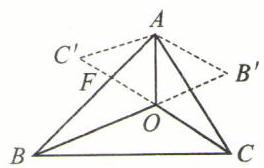
\includegraphics[width=0.2\textwidth]{bodyxb/src/bo_d20cdrf7aajc73bfmvhg_10_1228_1338_264_168_0.jpg}
\end{center}


(第 118 题)

过点 $A$ 分别作 ${BO},{CO}$ 的平行线,交 ${CO},{BO}$ 于 ${C}^{\prime },{B}^{\prime }$ 则 $\vv{OA} = \vv{O{B}^{\prime }} + \vv{O{C}^{\prime }}$ . 记 ${CO}$ 交 ${AB}$ 于点 $F.\because O$ 在 $\bigtriangleup {ABC}$ 内, $\therefore \vv{OB}$ 与 $\vv{OB}$ 反向. 又 $\dfrac{{S}_{\bigtriangleup {CBF}}}{{S}_{\bigtriangleup {CAF}}} = \dfrac{{S}_{\bigtriangleup {OBF}}}{{S}_{\bigtriangleup {DAF}}} = \dfrac{BF}{AF},\therefore \dfrac{{S}_{\bigtriangleup {COB}}}{{S}_{\bigtriangleup {COA}}}$  $= \dfrac{BF}{AF},\;\therefore \;\dfrac{\alpha }{\beta } = \dfrac{{S}_{\bigtriangleup {BOC}}}{{S}_{COA}} = \dfrac{BF}{AF}$ .

$\because A{B}^{\prime }//{OC}$ 即 ${OF}//{B}^{\prime }A,\therefore \dfrac{BF}{AF} = \dfrac{BO}{O{B}^{\prime }},\therefore \dfrac{\alpha }{\beta } = \dfrac{BO}{O{B}^{\prime }}$ 即 $\alpha  \cdot  O{B}^{\prime } = \beta  \cdot  {OB}.\therefore \alpha \vv{O{B}^{\prime }} + \beta \vv{OB} = \mathbf{0}$ .

同理, $\alpha \vv{O{C}^{\prime }} + \gamma \vv{OC} = \mathbf{0},\;\therefore \;\alpha \left( {\vv{O{B}^{\prime }} + \vv{O{C}^{\prime }}}\right)  + \beta \vv{OB} + \gamma \vv{OC} = \mathbf{0}$ ,即 $\alpha \vv{OA} + \beta \vv{OB} + \gamma \vv{OC} = \mathbf{0}$

119. D 提示: $a = \left( {-1, - 3}\right)  - \left( {3,1}\right)  = \left( {-4, - 4}\right)$ .

120. B 提示: $\vv{AD} = \vv{AB} + \vv{BC} + \vv{CD} = \left( {6,1}\right)  + \left( {-1,2}\right)  + \left( {2, - 3}\right)  = \left( {7,0}\right)$ .

121. B 提示: 设 $c = {\lambda a} + {\mu b}$ ,则 ${\lambda a} + {\mu b} = \lambda \left( {1,1}\right)  + \mu \left( {1, - 1}\right)  = \left( {\lambda  + \mu ,\lambda  - \mu }\right)  = c = \left( {-2,4}\right)$ .

$\therefore \left\{  \begin{array}{l} \lambda  + \mu  =  - 2, \\  \lambda  - \mu  = 4, \end{array}\right.$ 解得 $\left\{  {\begin{array}{l} \lambda  = 1, \\  \mu  =  - 3. \end{array}\;\therefore \;c = a - {3b}}\right.$ .

122. D 提示: $\vv{PQ} = \left( {-5,2}\right)  - \left( {3, - 6}\right)  = \left( {-8,8}\right) ,\vv{PR} = \left( {m, - 9}\right)  - \left( {3, - 6}\right)  = \left( {m - 3, - 3}\right)$ ,

$P,Q,R$ 三点共线 $\Leftrightarrow  \vv{PQ}//\vv{PR} \Rightarrow  \left( {-8}\right)  \cdot  \left( {-3}\right)  = 8 \cdot  \left( {m - 3}\right) .\;\therefore m = 6$ .

123. C 提示: $\vv{OM} = \vv{ON} - \vv{MN},\because \vv{AB} = \vv{MN},\therefore \vv{OM} = \vv{ON} - \vv{AB} = \left( {-2,0}\right)  - \left( {3, - 1}\right)  = \left( {-5,1}\right)$ .

124. D 提示: $\vv{OA} = \left( {4,2}\right) ,\vv{OB} = \left( {3,4}\right) ,\therefore 2\vv{OA} + \vv{OB} = 2 \cdot  \left( {4,2}\right)  + \left( {3,4}\right)  = \left( {{11},8}\right)$ .

125. D 提示:方法一:记 ${\theta }_{1} = {75}^{ \circ  },{\theta }_{2} = {15}^{ \circ  }$ ,则 $a - b = \left( {\cos {\theta }_{1},\sin {\theta }_{1}}\right)  - \left( {\cos {\theta }_{2},\sin {\theta }_{2}}\right)  = \left( {\cos {\theta }_{1} - \cos {\theta }_{2},\sin {\theta }_{1} - \sin {\theta }_{2}}\right)$ , $\left| {\vv{a} - \vv{b}}\right|  = \sqrt{{\left( \cos {\theta }_{1} - \cos {\theta }_{2}\right) }^{2} + {\left( \sin {\theta }_{1} - \sin {\theta }_{2}\right) }^{2}} = \sqrt{2 - 2\left( {\cos {\theta }_{1}\cos {\theta }_{2} + \sin {\theta }_{1}\sin {\theta }_{2}}\right) } = \sqrt{2 - 2\cos \left( {{\theta }_{1} - {\theta }_{2}}\right) } =$

$\sqrt{2 - 2\cos \left( {{75}^{ \circ  } - {15}^{ \circ  }}\right) } = \sqrt{2 - 2 \cdot  \dfrac{1}{2}} = 1.$

方法二:图解法. 点 $\left( {\cos {75}^{ \circ  },\sin {75}^{ \circ  }}\right)$ 和点 $\left( {\cos {15}^{ \circ  },\sin {15}^{ \circ  }}\right)$ 都是单位圆上的点. 且向量 $\vv{a},\vv{b}$ 的夹角是 ${75}^{ \circ  } - {15}^{ \circ  } = {60}^{ \circ  }$ ,故向量 $a,b,a - b$ 围成等边三角形. $\left| {a - b}\right|$ 等于单位圆的半径,为 1 .

126. A 提示: $\because a//b\therefore 3 \times  4 = 2 \cdot  x$ ,解得 $x = 6$ .

127. D 提示:由题意, $c =  - {2a} + {2b} =  - 2\left( {1, - 1}\right)  + 2\left( {2,1}\right)  = \left( {2,4}\right)$ ,设 $c = {\lambda m} + {\mu n} = \lambda \left( {-1,1}\right)  + \mu \left( {1,2}\right)  = \left( {-\lambda  + \mu ,\lambda  + {2\mu }}\right)$  $= \left( {2,4}\right) .\;\therefore \;\left\{  {\begin{array}{l}  - \lambda  + \mu  = 2, \\  \lambda  + {2\mu } = 4, \end{array}\text{ 解得 }\left\{  {\begin{array}{l} \lambda  = 0, \\  \mu  = 2. \end{array}\;\therefore \;c = 0\mathbf{m} + 2\mathbf{n}.}\right. }\right.$

128. C 提示: $\because a//b,\therefore \sin \alpha  \cdot  \cos \alpha  = \dfrac{3}{2} \cdot  \dfrac{1}{3} = \dfrac{1}{2}$ . 又 $\because \alpha$ 是锐角,且 $\sin \alpha  \cdot  \cos \alpha  = \dfrac{1}{2}\sin {2\alpha }$ ,

$\therefore \;\sin {2\alpha } = 1,{2\alpha } \in  \left( {0,\pi }\right) .\;\therefore \;{2\alpha } = \dfrac{\pi }{2},\alpha  = \dfrac{\pi }{4}$ .

129. D 提示: $\because \vv{PR} =  - 5\vv{QR},\therefore \vv{PR} = 5\vv{RQ}$ . 设 $R\left( {x,y}\right)$ ,根据定比分点的坐标公式有: $\left( {x,y}\right)  =$  $\left( {\dfrac{-1 + 5 \times  2}{1 + 5},\dfrac{-1 + 5 \times  5}{1 + 5}}\right)  = \left( {\dfrac{3}{2},4}\right) .$

130. D 提示: 将 $\vv{AP} = \vv{BP} - \vv{BA}$ 代入 $\vv{AP} = \dfrac{1}{3}\vv{PB}$ ,得 $\vv{BP} - \vv{BA} = \dfrac{1}{3}\vv{PB}$ ,即 $- \vv{PB} - \vv{BA} = \dfrac{1}{3}\vv{PB}$ ,得 $\dfrac{4}{3}\vv{PB} =  - \vv{BA}$ .

$\therefore \vv{PB} =  - \dfrac{3}{4}\vv{BA}$ .

131. A 提示: 设 $P\left( {x,0}\right)$ ,则 $\vv{{P}_{1}P} = \left( {x,0}\right)  - \left( {-1,2}\right)  = \left( {x + 1, - 2}\right) ,\vv{P{P}_{2}} = \left( {5,6}\right)  - \left( {x,0}\right)  = \left( {5 - x,6}\right)$ .

由 $\vv{{P}_{1}P} = \lambda \vv{P{P}_{2}}$ ,可得 $- 2 = {6\lambda }.\therefore \lambda  =  - \dfrac{1}{3}$ .

132. A 提示: 由已知,设 $\vv{b} = t\vv{a}$ ,其中 $t < 0$ ,故 $\left| \vv{b}\right|  =  - t\left| \vv{a}\right|  =  - \sqrt{5}t$ ,故 $t =  - 3$ . 故 $\vv{b} = \left( {-3,6}\right)$ .

133. B 提示: $\cos \theta  = \dfrac{\vv{a} \cdot  \vv{b}}{\left| \vv{a}\right|  \cdot  \left| \vv{b}\right| } = \dfrac{3 + 2}{\sqrt{10} \cdot  \sqrt{5}} = \dfrac{\sqrt{2}}{2},\theta  \in  \left\lbrack  {0,\pi }\right\rbrack  .\;\therefore \;\theta  = \dfrac{\pi }{4}$ .

134. A 提示: $\vv{CB} = \vv{AB} - \vv{AC} = \left( {k,1}\right)  - \left( {2,3}\right)  = \left( {k - 2, - 2}\right) ,\angle C = {90}^{ \circ  } \Rightarrow  \vv{AC}\bot \vv{CB} \Leftrightarrow  2\left( {k - 2}\right)  - 6 = 0$ ,

$\therefore k = 5$ .

135. A 提示: $D$ 的坐标是 $\left( {\dfrac{6 + 4}{2},\dfrac{1 + 3}{2}}\right)$ ,即 $D\left( {5,2}\right) ,\vv{AC} = \left( {4,3}\right)  - \left( {3,1}\right)  = \left( {1,2}\right) ,\left| \vv{AC}\right|  = \sqrt{5}$ ,

$\vv{DA} = \left( {3,1}\right)  - \left( {5,2}\right)  = \left( {-2, - 1}\right) ,\left| \vv{DA}\right|  = \sqrt{5} \cdot  \cos \theta  = \dfrac{\vv{AC} \cdot  \vv{DA}}{\left| \vv{AC}\right|  \cdot  \left| \vv{DA}\right| } = \dfrac{-2 - 2}{\sqrt{5} \cdot  \sqrt{5}} =  - \dfrac{4}{5}.$

136. D 提示: ${2a} - b = 2\left( {\cos \theta ,\sin \theta }\right)  - \left( {\sqrt{3}, - 1}\right)  = \left( {2\cos \theta  - \sqrt{3},2\sin \theta  + 1}\right) ,\left| {{2a} - b}\right|  = \sqrt{{\left( 2\cos \theta  - \sqrt{3}\right) }^{2} + {\left( 2\sin \theta  + 1\right) }^{2}} =$  $\sqrt{8 + 8\left( {\dfrac{1}{2}\sin \theta  - \dfrac{\sqrt{3}}{2}\cos \theta }\right) } = \sqrt{8 + 8\sin \left( {\theta  - \dfrac{\pi }{3}}\right) }.\;\because \;\sin \left( {\theta  - \dfrac{\pi }{3}}\right)  \in  \left\lbrack  {-1,1}\right\rbrack  ,\;\therefore \;\left| {{2a} - b}\right|  \in  \left\lbrack  {0,4}\right\rbrack  .$

137. $C$ 提示: 设 $c = \left( {x,y}\right)$ . 则 $a + b = \left( {1,2}\right)  + \left( {-2, - 4}\right)  = \left( {-1, - 2}\right) ,\left( {a + b}\right)  \cdot  c =  - x - {2y} = \dfrac{5}{2}$ ,即 $x + {2y} =  - \dfrac{5}{2}$ . 记 $a$ 与 $c$ 的夹角为 $\theta ,\theta  \in  \left\lbrack  {0,\pi }\right\rbrack  ,\cos \theta  = \dfrac{a \cdot  c}{\left| a\right|  \cdot  \left| c\right| } = \dfrac{x + {2y}}{\sqrt{5} \cdot  \sqrt{5}} =  - \dfrac{1}{2}.\;\therefore \;\theta  = \dfrac{2}{3}\pi$ .

138. $C$ 提示: $\vv{a}$ 在 $\vv{b}$ 方向上的数量投影是 $\left| \vv{a}\right|  \cdot  \cos \theta ,\theta$ 为 $\vv{a},\vv{b}$ 之间夹角, $\left| \vv{a}\right| \cos \theta  = \dfrac{\vv{a} \cdot  \vv{b}}{\left| \vv{b}\right| } = \dfrac{-8 + {21}}{\sqrt{{\left( -4\right) }^{2} + {7}^{2}}} = \dfrac{\sqrt{65}}{5}$ .

139. C 提示: $\vv{OP} = \vv{OA} + \vv{AP},\vv{AB} = \vv{OB} - \vv{OA},\therefore \vv{OA} \cdot  \vv{OP} = \vv{OA} \cdot  \left( {\vv{OA} + \vv{AP}}\right)  = \vv{OA} \cdot  \left( {\vv{OA} + t\vv{AB}}\right)  = \vv{OA} \cdot  (\vv{OA} + t\vv{OB}$  $- t\vv{OA}).\;\because \;\vv{OA} = \left( {3,0}\right) ,\vv{OB} = \left( {0,3}\right) ,\;\therefore \;\left| \vv{OA}\right|  = 3,\vv{OA} \cdot  \vv{OB} = 0\;\therefore \;\vv{OA} \cdot  \vv{OP} = \left( {1 - t}\right) {\vv{OA}}^{2} = 9\left( {1 - t}\right) ,t \in$  $\left\lbrack  {0,1}\right\rbrack  ,\;\therefore \;\vv{OA} \cdot  \vv{OP} \in  \left\lbrack  {0,9}\right\rbrack$ .

140. $\left( {1, - 1}\right) ,\left( {-4, - 3}\right)$ 提示: $a = \dfrac{\left( {a + b}\right)  + \left( {a - b}\right) }{2} = \dfrac{1}{2}\left\lbrack  {\left( {-3, - 4}\right)  + \left( {5,2}\right) }\right\rbrack   = \left( {1, - 1}\right)$ ,

$\vv{b} = \dfrac{\left( {\vv{a} + \vv{b}}\right)  - \left( {\vv{a} - \vv{b}}\right) }{2} = \dfrac{1}{2}\left\lbrack  {\left( {-3, - 4}\right)  - \left( {5,2}\right) }\right\rbrack   = \left( {-4, - 3}\right) .$

141. $\left( {-\sqrt{5}, - 2\sqrt{5}}\right)$ 提示: 设 $\vv{a} = \left( {x,y}\right)$ ,由 $\vv{a}//\vv{b}$ ,可得 ${2x} = y$ . 又 $\because \left| \vv{a}\right|  = 5,\therefore \sqrt{{x}^{2} + {y}^{2}} = 5$ . 解得 $\left\{  \begin{array}{l} x = \sqrt{5}, \\  y = 2\sqrt{5} \end{array}\right.$ 或 $\left\{  {\begin{array}{l} x =  - \sqrt{5}, \\  y =  - 2\sqrt{5}. \end{array}\text{ 又 }\because \;a,b}\right.$ 方向相反,故 $a = \left( {-\sqrt{5}, - 2\sqrt{5}}\right)$ .

142.(2,6)提示:向量 $\vv{a}$ 的终点是 $\left( {-2,1}\right)  + \left( {3,2}\right)  = \left( {1,3}\right)$ ,故向量 $2\vv{a}$ 的终点坐标是 $2\left( {1,3}\right)  = \left( {2,6}\right)$ .

143. 2 提示: $\lambda \vv{a} + \vv{b} = \lambda \left( {1,2}\right)  + \left( {2,3}\right)  = \left( {\lambda  + 2,{2\lambda } + 3}\right) ,\because \lambda \vv{a} + \vv{b}$ 与 $\mathbf{c}$ 共线,即 $\left( {\lambda \vv{a} + \vv{b}}\right) //\mathbf{c}$ ,

$\therefore  - 7 \cdot  \left( {\lambda  + 2}\right)  =  - 4\left( {{2\lambda } + 3}\right)$ ,解得 $\lambda  = 2$ .

144. $\left( {\dfrac{3}{5}, - \dfrac{4}{5}}\right)$ 或 $\left( {-\dfrac{3}{5},\dfrac{4}{5}}\right)$ 提示: 向量 $\vv{a}$ 的单位向量是 ${\vv{a}}_{0} = \dfrac{\vv{a}}{\left| \vv{a}\right| } = \dfrac{\left( 3, - 4\right) }{\sqrt{{3}^{2} + {\left( -4\right) }^{2}}} = \left( {\dfrac{3}{5}, - \dfrac{4}{5}}\right)$ ,而与向量 $\vv{a}$ 平行的单位向量是 $\pm  {a}_{0}$ ,即 $\left( {\dfrac{3}{5}, - \dfrac{4}{5}}\right)$ 或 $\left( {-\dfrac{3}{5},\dfrac{4}{5}}\right)$ .

145. 1,-2提示: $\lambda \vv{a} + \mu \vv{b} = \left( {{3\lambda } - {2\mu }, - {2\lambda } + \mu }\right)  = \mathbf{c} = \left( {7, - 4}\right) ,\left\{  \begin{array}{l} {3\lambda } - {2\mu } = 7, \\   - {2\lambda } + \mu  =  - 4, \end{array}\right.$ 解得 $\left\{  \begin{array}{l} \lambda  = 1, \\  \mu  =  - 2. \end{array}\right.$

146. $- 6, - \dfrac{8}{3}$ 提示: $- \dfrac{1}{2}a + \dfrac{3}{2}b =  - \dfrac{1}{2}\left( {x,2}\right)  + \dfrac{3}{2}\left( {-4,y}\right)  = \left( {-\dfrac{1}{2}x - 6, - 1 + \dfrac{3}{2}y}\right)  = c = \left( {-3, - 5}\right)$ , $\left\{  {\begin{array}{l}  - \dfrac{1}{2}x - 6 =  - 3, \\   - 1 + \dfrac{3}{2}y =  - 5, \end{array}\text{ 解得 }\left\{  \begin{array}{l} x =  - 6, \\  y =  - \dfrac{8}{3}. \end{array}\right. }\right.$

147. $\dfrac{2\pi }{3}$ 提示: $a//b \Leftrightarrow  \sin \alpha \cos \alpha  =  - \dfrac{\sqrt{3}}{2} \cdot  \dfrac{1}{2},\therefore \sin {2\alpha } = 2\sin \alpha \cos \alpha  =  - \dfrac{\sqrt{3}}{2}.\because \alpha$ 是钝角,

$\therefore {2\alpha } \in  \left( {\pi ,{2\pi }}\right) \;\therefore {2\alpha } = \dfrac{4}{3}\pi ,\alpha  = \dfrac{2}{3}\pi$ . 此时 $\vv{a},\vv{b}$ 不相等.

148. $\sqrt{2}$ 提示: $\vv{a} - \vv{b} = \left( {1,\sin \theta }\right)  - \left( {1,\cos \theta }\right)  = \left( {0,\sin \theta  - \cos \theta }\right) ,\;\therefore \left| {\vv{a} - \vv{b}}\right|  = \left| {\sin \theta  - \cos \theta }\right|  = \sqrt{2}\left| {\sin \left( {\theta  - \dfrac{\pi }{4}}\right) }\right|  \in  \left\lbrack  {0,\sqrt{2}}\right\rbrack$ , 即 $\left| {\vv{a} - \vv{b}}\right|$ 的最大值为 $\sqrt{2}$ .

149.(-2,10)提示: 记边 ${AB}$ 的中点为 $D$ ,则 $D$ 的坐标为 $\left( {\dfrac{-{10} + 6}{2},\dfrac{3 - 4}{2}}\right)$ ,即 $D\left( {-2, - \dfrac{1}{2}}\right)$ . 根据三角形重心的性质: 三角形的重心与顶点的距离等于它与对边中点的距离的两倍,即 $\vv{CM} = 2\vv{MD}$ ,设 $C\left( {x,y}\right)$ ,根据定比分点的坐标公式可得点 $M$ 的坐标为 $\left( {\dfrac{x + 2 \times  \left( {-2}\right) }{1 + 2},\dfrac{y + 2 \times  \left( {-\dfrac{1}{2}}\right) }{1 + 2}}\right)$ ,即 $M\left( {\dfrac{x - 4}{3},\dfrac{y - 1}{3}}\right)$ . 已知 $M\left( {-2,3}\right)$ ,则 $\left\{  \begin{array}{l} \dfrac{x - 4}{3} =  - 2, \\  \dfrac{y - 1}{3} = 3, \end{array}\right.$ 解得 $\left\{  \begin{array}{l} x =  - 2, \\  y = {10}. \end{array}\right.$ 即顶点 $C$ 的坐标为(-2,10).

150. 设起点坐标为(x, y),有 $\left( {0,0}\right)  - \left( {x,y}\right)  = \left( {-x, - y}\right)  =  - \left( {x,y}\right)  = \left( {-4,2}\right)$ ,故 $a$ 的起点坐标为 $\left( {x,y}\right)  = \left( {4, - 2}\right)$ .

151. 据题意,设点 $C$ 的坐标为 $C\left( {x,y}\right)$ ,则有 $\left( {x,y}\right)  = \alpha \left( {3,1}\right)  + \beta \left( {-1,3}\right) .\;\therefore \left\{  \begin{array}{l} x = {3\alpha } - \beta , \\  y = \alpha  + {3\beta }, \end{array}\right.$ 整理得 $\left\{  \begin{array}{l} \alpha  = \dfrac{{3x} + y}{10}, \\  \beta  = \dfrac{{3y} - x}{10}\text{ . 代入 }\alpha  + \beta  \end{array}\right.$  $= 1$ ,整理得 $x + {2y} - 5 = 0$ . 又 $\alpha ,\beta  \in  \mathbf{R}$ ,故点 $C$ 的轨迹是直线 $x + {2y} - 5 = 0$ .

152. (1) $\vv{AB} = \left( {-2, - 2}\right)  - \left( {3,1}\right)  = \left( {-5, - 3}\right)$ . 若设 $D\left( {x,y}\right)$ ,则 $\vv{CD} = \left( {x,y}\right)  - \left( {-1,4}\right)  = \vv{AB} = \left( {-5, - 3}\right)$ ,故 $\left( {x,y}\right)  =$  $\left( {-1,4}\right)  + \left( {-5, - 3}\right)  = \left( {-6,1}\right)$ ,即点 $D$ 的坐标为(-6,1).

(2) $O$ 为原点, $\vv{OP} = \vv{AB} = \left( {-5, - 3}\right)$ ,故点 $P$ 的坐标为(-5, - 3).

153. $\vv{AB} = \left( {n + 2,1 - m}\right) ,\vv{AC} = \left( {7, - 1 - m}\right)$ .

$\because$ 点 $A,B,C$ 三点共线, $\therefore \vv{AB},\vv{AC}$ 平行, $\therefore \left( {n + 2}\right) \left( {-1 - m}\right)  - 7\left( {1 - m}\right)  = 0$ .

又 $\because m = {2n}$ ,代入上式,得 $\left\{  \begin{array}{l} m = 6, \\  n = 3 \end{array}\right.$ 或 $\left\{  \begin{array}{l} m = 3, \\  n = \dfrac{3}{2}. \end{array}\right.$

154. $\vv{a} + x\vv{b} = \left( {3,4}\right)  + x\left( {2, - 1}\right)  = \left( {{2x} + 3,4 - x}\right) ,\vv{a} - \vv{b} = \left( {3,4}\right)  - \left( {2, - 1}\right)  = \left( {1,5}\right) .\left( {\vv{a} + x\vv{b}}\right) //\left( {\vv{a} - \vv{b}}\right)  \Leftrightarrow  5\left( {{2x} + 3}\right)  = 1 \cdot  (4 -$  $x)$ ,解得 $x =  - 1$ .

155. 假设存在,则有 $\left( {6,4}\right)  = x\left( {8,2}\right)  + y\left( {3,3}\right)  + z\left( {6,{12}}\right)$ ,可得 $\left\{  \begin{array}{l} {8x} + {3y} + {6z} = 6, \\  {2x} + {3y} + {12z} = 4, \\  x + y + z = 1, \end{array}\right.$ 解得 $y = \dfrac{1}{3}$ ,存在.

156. 由题意可知, $\vv{AP} = \dfrac{1}{3}\vv{AB}$ 或 $\vv{AP} =  - \dfrac{1}{3}\vv{AB}$ . 设点 $P\left( {x,y}\right)$ ,则 $\vv{AP} = \left( {x - 3,y}\right) ,\vv{AB} = \left( {-4, - 6}\right)$ .

$\therefore \left\{  \begin{array}{l} x - 3 =  - \dfrac{4}{3}, \\  y =  - 2 \end{array}\right.$ 或 $\left\{  \begin{array}{l} x - 3 = \dfrac{4}{3}, \\  y = 2. \end{array}\right.$ 得点 $P\left( {\dfrac{5}{3}, - 2}\right)$ 或点 $P\left( {\dfrac{13}{3},2}\right)$ .

157. $\left| \mathbf{c}\right|  = 4,\vv{b} \cdot  \mathbf{c} = \left| \vv{b}\right| \left| \mathbf{c}\right| \cos {120}^{ \circ  } =  - 4 \Rightarrow  \left| \vv{b}\right|  = 2$ .

$\left\{  {\begin{array}{l} \vv{a} \cdot  \mathbf{c} = m{\vv{a}}^{2} + n\vv{a} \cdot  \vv{b} = 0, \\  \mathbf{c} \cdot  \mathbf{c} = m\vv{a} \cdot  \mathbf{c} + n\vv{b} \cdot  \mathbf{c} = {16}, \\  \vv{b} \cdot  \mathbf{c} = m\vv{a} \cdot  \vv{b} + n\vv{b} \cdot  \vv{b} =  - 4 \end{array} \Rightarrow  \left\{  {\begin{array}{l} m =  \pm  \sqrt{6}, \\  n =  - 4, \\  \vv{a} \cdot  \vv{b} =  \pm  2\sqrt{6} \end{array} \Rightarrow  \cos \theta  =  \pm  \dfrac{\sqrt{3}}{2},\;\therefore \;\theta  = {30}^{ \circ  }\text{ 或 }\theta  = {150}^{ \circ  }.}\right. }\right.$

158. B 提示: $\vv{BC} = \vv{AD} = \vv{AB} + \vv{BD},\therefore \vv{BD} = \vv{BC} - \vv{AB}$ ,另 $\vv{BC} = \vv{AC} - \vv{AB}$ ,代入得 $\vv{BD} = \vv{AC} - \vv{AB} - \vv{AB} = \vv{AC} - 2\vv{AB} =$  $\left( {1,3}\right)  - 2\left( {2,4}\right)  = \left( {-3, - 5}\right)$ .

159. B 提示: 设动点 $P\left( {x,y}\right)$ ,则 $\vv{AP} = \left( {x,y}\right)  - \left( {1,1}\right)  = \left( {x - 1,y - 1}\right) ,\vv{OB} = \left( {4, - 6}\right) ,\vv{AP}//\vv{OB} \Leftrightarrow   - 6\left( {x - 1}\right)  = 4\left( {y - 1}\right)$ ,整理得 ${3x} + {2y} - 5 = 0$ .

160. B 提示: $\vv{AB} = \left( {4,5}\right)  - \left( {1,2}\right)  = \left( {3,3}\right) ,\vv{BC} = \left( {2,3}\right)  - \left( {4,5}\right)  = \left( {-2, - 2}\right)$ ,由 $\vv{AB} = \lambda \vv{BC}$ ,有 $3 =  - {2\lambda },\lambda  =  - \dfrac{3}{2}$ .

161. A 提示:方法一:设点 $R\left( {x,y}\right)$ ,则 $\vv{PS} = \left( {4,0}\right)  - \left( {0,3}\right)  = \left( {4, - 3}\right)$ , $\left| \vv{PS}\right|  = \sqrt{{4}^{2} + {\left( -3\right) }^{2}} = 5$ , $\vv{SR} = \left( {x,y}\right)  - \left( {4,0}\right)  =$  $\left( {x - 4,y}\right) ,\left| \vv{SR}\right|  = \sqrt{{\left( x - 4\right) }^{2} + {y}^{2}},\vv{RP} = \left( {0,3}\right)  - \left( {x,y}\right)  = \left( {-x,3 - y}\right) ,\left| \vv{RP}\right|  = \sqrt{{x}^{2} + {\left( y - 3\right) }^{2}}$ ,由于 ${PQRS}$ 为正方形, $\left| \vv{PS}\right|  = \left| \vv{SR}\right|  \Rightarrow  {\left( x - 4\right) }^{2} + {y}^{2} = {25},\left| \vv{RP}\right|  = \sqrt{2}\left| \vv{PS}\right|  \Rightarrow  {x}^{2} + {\left( y - 3\right) }^{2} = {50}$ ,联立后可解得 $\left\{  \begin{array}{l} x = 7, \\  y = 4, \end{array}\right.$ 或 $\left\{  \begin{array}{l} x = 1, \\  y =  - 4. \end{array}\right.$ (舍去,因为原点不在正方形 ${PQRS}$ 内) $\therefore \vv{RM} = \dfrac{1}{2}\vv{RP} = \dfrac{1}{2}\left( {-7,3 - 4}\right)  = \left( {-\dfrac{7}{2}, - \dfrac{1}{2}}\right)$ .

方法二: $\vv{RM} = \dfrac{1}{2}\vv{RP},\vv{SP} = \vv{OP} - \vv{OS} = \left( {0,3}\right)  - \left( {4,0}\right)  = \left( {-4,3}\right) ,\left| \vv{SP}\right|  = \sqrt{{\left( -4\right) }^{2} + {3}^{2}} = 5$ . 设 $\vv{SR} = \left( {x,y}\right)$ ,由于 ${PQRS}$ 是正方形, $\left| \vv{SR}\right|  = \left| \vv{SP}\right|  = 5$ ,即 $\sqrt{{x}^{2} + {y}^{2}} = 5$ ,又 $\because \vv{SR}\bot \vv{SP} \Leftrightarrow   - {4x} + {3y} = 0$ . 联立后解得 $\left\{  \begin{array}{l} x = 3, \\  y = 4, \end{array}\right.$ 或 $\left\{  \begin{array}{l} x =  - 3, \\  y =  - 4. \end{array}\right.$ (舍去, 因为原点不在正方形 ${PQRS}$ 内) $\therefore \vv{RM} = \dfrac{1}{2}\vv{RP} = \dfrac{1}{2}\left( {\vv{SP} - \vv{SR}}\right)  = \dfrac{1}{2}\left\lbrack  {\left( {-4,3}\right)  - \left( {3,4}\right) }\right\rbrack   = \left( {-\dfrac{7}{2}, - \dfrac{1}{2}}\right)$ .

162. A 提示: 重心 $M$ 的坐标为 $M\left( {\dfrac{1 + 5 + 3}{3},\dfrac{4 + 0 + \left( {-3}\right) }{3}}\right)$ ,即 $M\left( {3,\dfrac{1}{3}}\right)$ ,点 $M$ 关于原点 $O$ 对称的点 $N$ 的坐标为 $\left( {-3, - \dfrac{1}{3}}\right)$ .

163. $C$ 提示: $\vv{BC} = \left( {\sqrt{3},0}\right)  - \left( {0,0}\right)  = \left( {\sqrt{3},0}\right) ,\vv{AC} = \left( {\sqrt{3},0}\right)  - \left( {\sqrt{3},1}\right)  = \left( {0, - 1}\right) ,\angle {ACB} = \dfrac{\pi }{2},\left| \vv{BC}\right|  = \sqrt{3},\left| \vv{AC}\right|  = 1$ .

$\therefore \tan \angle {BAC} = \dfrac{\left| \vv{BC}\right| }{\left| \vv{AC}\right| } = \sqrt{3},\angle {BAC} = \dfrac{\pi }{3},\angle {EAC} = \dfrac{1}{2}\angle {BAC} = \dfrac{\pi }{6},\tan \angle {EAC} = \dfrac{\left| \vv{CE}\right| }{\left| \vv{AC}\right| } = \dfrac{\left| \vv{EC}\right| }{1} = \dfrac{\sqrt{3}}{3}$ ,

$\therefore \left| \vv{BC}\right|  = \sqrt{3} = 3\left| \vv{CE}\right| \;\therefore \;\vv{BC} =  \pm  3\vv{CE}$ . 结合图形可知 $\vv{BC} =  - 3\vv{CE},\lambda  =  - 3$ .

164. A 提示: $\vv{BC} = \left( {3,1}\right)  - \left( {-1, - 2}\right)  = \left( {4,3}\right)$ . 由 $\vv{BC} = 2\vv{AD}$ ,得 $\vv{AD} = \dfrac{1}{2}\vv{BC} = \left( {2,\dfrac{3}{2}}\right)$ , $\vv{OD} = \vv{AD} + \vv{OA} = \left( {2,\dfrac{3}{2}}\right)  + \left( {0,2}\right)$  $= \left( {2,\dfrac{7}{2}}\right) ,O$ 为原点,故点 $D$ 的坐标为 $\left( {2,\dfrac{7}{2}}\right)$ .

165. A 提示: 设向量 $\vv{a} = \left( {m,n}\right)$ ,对函数 $y = {2}^{x} + 1$ 上的任意点(x, y),在向量 $\vv{a}$ 的作用下,变为 $\left( {{x}^{\prime },{y}^{\prime }}\right) ,\left\{  \begin{array}{l} {x}^{\prime } - x = m, \\  {y}^{\prime } - y = n, \end{array}\right.$ 即 $\left\{  \begin{array}{l} x = {x}^{\prime } - m, \\  y = {y}^{\prime } - n. \end{array}\right.$ 代入 $y = {2}^{x} + 1$ ,得 ${y}^{\prime } - n = {2}^{{x}^{\prime } - m} + 1$ ,即 ${y}^{\prime } = {2}^{{x}^{\prime } - m} + \left( {n + 1}\right)$ ,对比平移后的函数 $y = {2}^{x + 1}$ ,知 $\left\{  \begin{array}{l} m =  - 1, \\  n =  - 1. \end{array}\right.$ 故 $a$  $= \left( {-1, - 1}\right)$ .

166. D 提示: 设 $\vv{OC} = \left( {x,y}\right)$ ,则 $\vv{AC} = \vv{OC} - \vv{OA} = \left( {x,y}\right)  - \left( {4,6}\right)  = \left( {x - 4,y - 6}\right) ,\vv{OC}\bot \vv{OA} \Leftrightarrow  {4x} + {6y} = 0$ ,

$\vv{AC}//\vv{OB} \Leftrightarrow  3\left( {y - 6}\right)  = 5\left( {x - 4}\right)$ ,联立得 $\left\{  \begin{array}{l} {4x} + {6y} = 0, \\  3\left( {y - 6}\right)  = 5\left( {x - 4}\right) , \end{array}\right.$ 解得 $\left\{  \begin{array}{l} x = \dfrac{2}{7}, \\  y =  - \dfrac{4}{21}, \end{array}\right.$ 即 $\vv{OC} = \left( {\dfrac{2}{7}, - \dfrac{4}{21}}\right)$ .

167. D 提示: ${ma} + {nb} = m\left( {1,1}\right)  + n\left( {1, - 1}\right)  = \left( {m + n,m - n}\right)  = c = \left( {\sqrt{2}\cos \alpha ,\sqrt{2}\sin \alpha }\right)$ . 方法一: $\therefore \left\{  {\begin{array}{l} \dfrac{m + n}{\sqrt{2}} = \cos \alpha , \\  \dfrac{m - n}{\sqrt{2}} = \sin \alpha  \end{array} \Rightarrow  }\right.$

$\dfrac{{\left( m + n\right) }^{2}}{2} + \dfrac{{\left( m - n\right) }^{2}}{2} = 1.\;\therefore {m}^{2} + {n}^{2} = 1$ ,点(m, n)的轨迹是以(0,0)为圆心,1 为半径的圆,记 $l = {\left( m - 3\right) }^{2} + {n}^{2}$ ,事实上, $l$ 是点(m, n)到点(3,0)的距离的平方. $\therefore {l}_{\max } = {\left( 3 + 1\right) }^{2} = {16}$ ,此时 $m =  - 1,n = 0$ .

方法二: $l$ 的最大值也可通过如下过程求得 $l = {\left( m - 3\right) }^{2} + {n}^{2} = {n}^{2} + {m}^{2} - {6m} + 9 = {10} - {6m},m = \dfrac{\sqrt{2}}{2}\cos \alpha  + \dfrac{\sqrt{2}}{2}\sin \alpha  =$  $\cos \left( {\alpha  - \dfrac{\pi }{4}}\right)  \in  \left\lbrack  {-1,1}\right\rbrack$ ,故 ${l}_{\max } = {16}$ ,此时 $m =  - 1,n = 0$ .

168. C 提示: $\vv{OA} = \vv{OC} + \vv{CA} = \left( {\sqrt{2}\cos \alpha  + 2,\sqrt{2}\sin \alpha  + 2}\right)$ ,设点 $A$ 的坐标为(x, y),则由 $\left\{  \begin{array}{l} x = \sqrt{2}\cos \alpha  + 2, \\  y = \sqrt{2}\sin \alpha  + 2, \end{array}\right.$ 得 ${\left( x - 2\right) }^{2} + {\left( y - 2\right) }^{2} = 2$ ,即点 $A$ 的轨迹是以(2,2)为圆心, $\sqrt{2}$ 为半径的圆 $\odot  C.\vv{OA}$ 与 $\vv{OB}$ 的夹角为 $\angle {AOB}$ ,为求该角范围,从点 $O$ 向 $\odot  C$ 作切线,切点为 ${A}_{1},{A}_{2}$ (如图). $\angle {CO}{A}_{1} = \angle {CO}{A}_{2}.\sin \angle {CO}{A}_{1} = \dfrac{\left| C{A}_{1}\right| }{\left| CO\right| } = \dfrac{\sqrt{2}}{2\sqrt{2}} = \dfrac{1}{2}.\;\therefore \angle {CO}{A}_{1} =$  $\angle {CO}{A}_{2} = \dfrac{\pi }{6},\angle {COB} = \dfrac{\pi }{4}.\;\therefore \angle {AOB}$ 的取值范围是 $\left\lbrack  {\dfrac{\pi }{4} - \dfrac{\pi }{6},\dfrac{\pi }{4} + \dfrac{\pi }{6}}\right\rbrack$ , 即 $\left\lbrack  {\dfrac{\pi }{12},\dfrac{5\pi }{12}}\right\rbrack$ .

\begin{center}
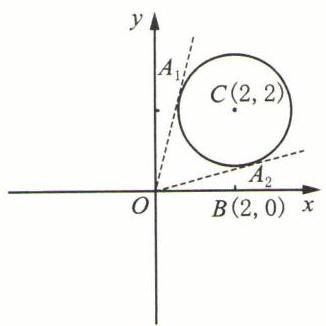
\includegraphics[width=0.2\textwidth]{bodyxb/src/bo_d20cdrf7aajc73bfmvhg_14_1173_397_326_326_0.jpg}
\end{center}


(第 168 题)

169. $- \dfrac{1}{3}$ 提示: $k\vv{a} + \vv{b} = k\left( {1,2}\right)  + \left( {-3,2}\right)  = \left( {k - 3,{2k} + 2}\right) ,\vv{a} - 3\vv{b} = \left( {1,2}\right)  - 3\left( {-3,2}\right)  = \left( {{10}, - 4}\right) ,\left( {k\vv{a} + \vv{b}}\right) //\left( {\vv{a} - 3\vv{b}}\right)  \Leftrightarrow$  $- 4\left( {k - 3}\right)  = {10}\left( {{2k} + 2}\right)$ ,解得 $k =  - \dfrac{1}{3}$ .

170. (4,23) 提示: $\vv{OP}\left( t\right)  = \vv{OP}\left( 0\right)  + v \cdot  t = \left( {-6, - 2}\right)  + t\left( {2,5}\right)  = \left( {{2t} - 6,{5t} - 2}\right)$ ,代入 $t = 5$ ,得 $\vv{OP}\left( 5\right)  = \left( {4,{23}}\right)$ ,即为此时点 $P$ 的坐标.

171. (21,-28) 提示: $\vv{MN} = \vv{CN} - \vv{CM} = 3\vv{CB} + 2\vv{CA},\vv{CB} = \left( {3, - 4}\right)  - \left( {-2,4}\right)  = \left( {5, - 8}\right) ,\vv{CA} = \left( {1,2}\right)  - \left( {-2,4}\right)  = \left( {3, - 2}\right)$ , $\vv{MN} = 3\vv{CB} + 2\vv{CA} = 3\left( {5, - 8}\right)  + 2\left( {3, - 2}\right)  = \left( {{21}, - {28}}\right)$ .

172. $\left\lbrack  {-6,2}\right\rbrack$ 提示: $\vv{a} + \vv{b} = \left( {-2,2}\right)  + \left( {5,k}\right)  = \left( {3,k + 2}\right) ,\left| {\vv{a} + \vv{b}}\right|  \leq  5 \Leftrightarrow  \sqrt{{3}^{2} + {\left( k + 2\right) }^{2}} \leq  5$ ,解得 $- 6 \leq  k \leq  2$ .

173. $- \dfrac{2}{3}$ 提示: $\vv{AB} = \vv{OB} - \vv{OA} = \left( {4,5}\right)  - \left( {k,{12}}\right)  = \left( {4 - k, - 7}\right) ,\vv{AC} = \vv{OC} - \vv{OA} = \left( {-k,{10}}\right)  - \left( {k,{12}}\right)  = \left( {-{2k}, - 2}\right) ,A,B$  $C$ 三点共线 $\Leftrightarrow  \vv{AB}//\vv{AC} \Leftrightarrow   - 2\left( {4 - k}\right)  =  - 7\left( {-{2k}}\right)$ ,解得 $k =  - \dfrac{2}{3}$ .

174. $1 + \sqrt{2}$ 提示: $\vv{AB} = \left( {2,{a}^{2}}\right)  - \left( {1, - a}\right)  = \left( {1,{a}^{2} + a}\right) ,\vv{AC} = \left( {3,{a}^{3}}\right)  - \left( {1, - a}\right)  = \left( {2,{a}^{3} + a}\right)$ . $A,B,C$ 三点共线 $\Leftrightarrow  \vv{AB}//\vv{AC}$  $\Leftrightarrow  1 \cdot  \left( {{a}^{3} + a}\right)  = 2\left( {{a}^{2} + a}\right)$ . 解得 ${a}_{1} = 0,{a}_{2,3} = 1 \pm  \sqrt{2}$ . 又 $a > 0$ ,故 $a = 1 + \sqrt{2}$ .

175. $\dfrac{9}{5}$ 提示: $\lambda \vv{a} + \vv{b} = \lambda \left( {2,1}\right)  + \left( {1,1}\right)  = \left( {{2\lambda } + 1,\lambda  + 1}\right) ,\left| {\lambda \vv{a} + \vv{b}}\right|  = \sqrt{{\left( 2\lambda  + 1\right) }^{2} + {\left( \lambda  + 1\right) }^{2}} = \sqrt{29}$ ,解得 ${\lambda }_{1} =  - 3,{\lambda }_{2} = \dfrac{9}{5}$ . 又 $\lambda  > 0$ ,故 $\lambda  = \dfrac{9}{5}$ .

176. $\left( {-\dfrac{\sqrt{10}}{5},\dfrac{3\sqrt{10}}{5}}\right)$ 提示:方法一:记 $\angle {AOB} = \theta$ ,则 $\theta  \in  \left( {0,\dfrac{\pi }{2}}\right) ,\tan \theta  = \dfrac{3}{4}$ . 易知 $\cos \theta  = \dfrac{4}{5}$ .

利用 $\cos \theta  = 2{\cos }^{2}\dfrac{\theta }{2} - 1 = 1 - 2{\sin }^{2}\dfrac{\theta }{2}$ ,可求得 $\cos \dfrac{\theta }{2} = \dfrac{3}{\sqrt{10}},\sin \dfrac{\theta }{2} = \dfrac{1}{\sqrt{10}}$ . 由 $\left| \vv{OC}\right|  = 2$ 并结合图形,

可得 $\vv{OC} = 2\left( {\cos \left( {\dfrac{\theta }{2} + \dfrac{\pi }{2}}\right) ,\sin \left( {\dfrac{\theta }{2} + \dfrac{\pi }{2}}\right) }\right)  = 2\left( {-\sin \dfrac{\theta }{2},\cos \dfrac{\theta }{2}}\right)  = \left( {-\dfrac{\sqrt{10}}{5},\dfrac{3\sqrt{10}}{5}}\right)$ .

方法二:记 $\angle {AOB} = \theta$ ,则 $\angle {COA} = \angle {COB} = \dfrac{\theta }{2}$ ,设 $\vv{OC} = \left( {x,y}\right) .\because \vv{OA} = \left( {0,1}\right) ,\therefore \left| \vv{OA}\right|  = 1$ . 又 $\because \vv{OB} =$  $\left( {-3,4}\right) ,\therefore \left| \vv{OB}\right|  = 5$ . 利用向量的数量积: $\vv{OC} \cdot  \vv{OA} = y = \left| \vv{OC}\right|  \cdot  \left| \vv{OA}\right|  \cdot  \cos \dfrac{\theta }{2} = \left| \vv{OC}\right|  \cdot  \cos \dfrac{\theta }{2},\vv{OC} \cdot  \vv{OB} =  - {3x}$  $+ {4y} = \left| \vv{OC}\right|  \cdot  \left| \vv{OB}\right|  \cdot  \cos \dfrac{\theta }{2} = \left| \vv{OC}\right|  \cdot  5\cos \dfrac{\theta }{2}$ ,可得 $- {3x} + {4y} = {5y}$ ,即 $y =  - {3x}.\left| \vv{OC}\right|  = 2 \Leftrightarrow  \sqrt{{x}^{2} + {y}^{2}} = 2$ . 联立得 $\left\{  {\begin{array}{l} y =  - {3x}, \\  {x}^{2} + {y}^{2} = 4, \end{array}\text{ 解得 }\left\{  {\begin{array}{l} x = \dfrac{\sqrt{10}}{5}, \\  y =  - \dfrac{3\sqrt{10}}{5}, \end{array}\text{ 或 }\left\{  {\begin{array}{l} x =  - \dfrac{\sqrt{10}}{5}, \\  y = \dfrac{3\sqrt{10}}{5}. \end{array}\text{ 结合图形,知 }x < 0,y > 0,\text{ 故 }\vv{OC} = \left( {x,y}\right)  = \left( {-\dfrac{\sqrt{10}}{5},\dfrac{3\sqrt{10}}{5}}\right) .}\right. }\right. }\right.$

177. -4,2,1 提示: ${\lambda }_{1}{\vv{a}}_{1} + {\lambda }_{2}{\vv{a}}_{2} + {\lambda }_{3}{\vv{a}}_{3} = \left( {{\lambda }_{1} + {\lambda }_{2} + 2{\lambda }_{3}, - {\lambda }_{2} + 2{\lambda }_{3}}\right)  = \mathbf{0} \Rightarrow  \left\{  {\begin{array}{l} {\lambda }_{1} + {\lambda }_{2} + 2{\lambda }_{3} = 0, \\   - {\lambda }_{2} + 2{\lambda }_{3} = 0 \end{array} \Rightarrow  \left\{  \begin{array}{l} {\lambda }_{1} =  - 4{\lambda }_{3}, \\  {\lambda }_{2} = 2{\lambda }_{3} \end{array}\right. }\right.$  $\therefore {\lambda }_{1} : {\lambda }_{2} : {\lambda }_{3} = \left( {-4}\right)  : 2 : 1.{\lambda }_{1},{\lambda }_{2},{\lambda }_{3}$ 可取-4,2,1.

178. 方法一: 设点 $B\left( {m,n}\right)$ ,则 $\vv{OB} = \left( {m,n}\right) ,\left| \vv{OB}\right|  = \sqrt{{m}^{2} + {n}^{2}},\vv{OA} = \left( {5,2}\right) ,\left| \vv{OA}\right|  = \sqrt{{5}^{2} + {2}^{2}} = \sqrt{29},\vv{AB} = \vv{OB} - \vv{OA} = (m$  $- 5,n - 2),\left| \vv{AB}\right|  = \sqrt{{\left( m - 5\right) }^{2} + {\left( n - 2\right) }^{2}}$ ,由于 $\bigtriangleup {OAB}$ 为等腰直角三角形且 $\angle A = {90}^{ \circ  }$ ,故 $\left| \vv{OB}\right|  = \sqrt{2}\left| \vv{OA}\right|  \Rightarrow  {m}^{2} + {n}^{2} =$  ${58},\left| \vv{OA}\right|  = \left| \vv{AB}\right|  \Rightarrow  {10m} + {4n} = {58}$ . 联立得 $\left\{  \begin{array}{l} {m}^{2} + {n}^{2} = {58}, \\  {5m} + {2n} = {29}, \end{array}\right.$ 解得 $\left\{  \begin{array}{l} m = 3, \\  n = 7, \end{array}\right.$ 或 $\left\{  \begin{array}{l} m = 7, \\  n =  - 3. \end{array}\right.$ 当点 $B$ 的坐标为 $B\left( {3,7}\right)$ 时, $\vv{AB} =$ (-2,5),当点 $B$ 的坐标为 $B\left( {7, - 3}\right)$ 时, $\vv{AB} = \left( {2, - 5}\right)$ .

方法二: 设 $\vv{AB} = \left( {x,y}\right) ,\vv{AO} = \left( {0,0}\right)  - \left( {5,2}\right)  = \left( {-5, - 2}\right) ,\left| \vv{AO}\right|  = \sqrt{{5}^{2} + {2}^{2}} = \sqrt{29},\because \bigtriangleup {OAB}$ 为等腰直角三角形且 $\angle A = {90}^{ \circ  },\therefore \left| \vv{AB}\right|  = \sqrt{{x}^{2} + {y}^{2}} = \left| \vv{AO}\right|  = \sqrt{29}$ . 利用向量的数量积: $\vv{AO}\bot \vv{AB} \Leftrightarrow   - {5x} - {2y} = 0$ . 联立得 $\left\{  \begin{array}{l} {x}^{2} + {y}^{2} = {29}, \\  {5x} + {2y} = 0, \end{array}\right.$ 解得 $\left\{  \begin{array}{l} x = 2, \\  y =  - 5 \end{array}\right.$ 或 $\left\{  \begin{array}{l} x =  - 2, \\  y = 5. \end{array}\right.$ 当 $\vv{AB}$ 取(2, - 5)时, $\vv{OB} = \vv{OA} + \vv{AB} = \left( {5,2}\right)  + \left( {2, - 5}\right)  = \left( {7, - 3}\right)$ ,即点 $B$ 的坐标为(7, - 3). 当 $\vv{AB}$ 取(-2,5)时, $\vv{OB} = \vv{OA} + \vv{AB} = \left( {5,2}\right)  + \left( {-2,5}\right)  = \left( {3,7}\right)$ ,即点 $B$ 的坐标为(3,7).

179. 设点 $P$ 的坐标为(x, y),则 $\vv{OP} = {2a} + {tb} = \left( {2 + t,t}\right)  \Rightarrow  \left\{  {\begin{array}{l} x = 2 + t, \\  y = t \end{array} \Rightarrow  x - y - 2 = 0}\right. ,\vv{OQ} = {ta} - {2b} = \left( {t - 2, - 2}\right)  \Rightarrow$  $\left\{  {\begin{array}{l} x = t - 2, \\  y =  - 2 \end{array} \Rightarrow  y =  - 2}\right.$ . 由 $\left\{  {\begin{array}{l} x - y - 2 = 0, \\  y =  - 2 \end{array} \Rightarrow  \left\{  \begin{array}{l} x = 0, \\  y =  - 2, \end{array}\right. }\right.$ 得证.

180. 由题意得 $x \bot  y \Rightarrow  x \cdot  y = 0,\left| a\right|  = 2,\left| b\right|  = 1,a \cdot  b = 0,\;\therefore \left\lbrack  {a + \left( {{t}^{2} - 3}\right) b}\right\rbrack  \left\lbrack  {-{ka} + {tb}}\right\rbrack   =  - k{\left| a\right| }^{2} + \left( {t - k{t}^{2} + {3k}}\right) a \cdot  b +$  $t\left( {{t}^{2} - 3}\right) {\left| \vv{b}\right| }^{2} =  - {4k} + t\left( {{t}^{2} - 3}\right)  = 0,\;\therefore \;k = \dfrac{{t}^{3} - {3t}}{4}\left( {t \neq  0\text{ 且 }t \neq   \pm  \sqrt{3}}\right) ,\;\therefore \;\dfrac{k + {t}^{2}}{t} = \dfrac{{t}^{2} + {4t} - 3}{4} = \dfrac{{\left( t + 2\right) }^{2} - 7}{4}$ . 当 $t =  - 2$ 时, $\dfrac{k + {t}^{2}}{t}$ 有最小值 $- \dfrac{7}{4}$ ,此时 $k =  - \dfrac{1}{2},x = a + b = \left( {\dfrac{1}{2} + \sqrt{3},\dfrac{\sqrt{3}}{2} - 1}\right)  \neq  0,y = \dfrac{1}{2}a - {2b} =$  $\left( {\dfrac{\sqrt{3}}{2} - 1, - \dfrac{1}{2} - \sqrt{3}}\right)  \neq  \mathbf{0}.$

181. (1) $a \bot  b \Leftrightarrow  a \cdot  b = 0,\therefore \sin \theta  + \cos \theta  = \sqrt{2}\sin \left( {\theta  + \dfrac{\pi }{4}}\right)  = 0,\;\because \theta  \in  \left( {-\dfrac{\pi }{2},\dfrac{\pi }{2}}\right) ,\therefore \theta  + \dfrac{\pi }{4} \in  \left( {-\dfrac{\pi }{4},\dfrac{3}{4}\pi }\right)$ , $\therefore \theta  + \dfrac{\pi }{4} = 0,\theta  =  - \dfrac{\pi }{4}$ .

(2) $\vv{a} + \vv{b} = \left( {\sin \theta ,1}\right)  + \left( {1,\cos \theta }\right)  = \left( {\sin \theta  + 1,\cos \theta  + 1}\right) ,\left| {\vv{a} + \vv{b}}\right|  = \sqrt{{\left( \sin \theta  + 1\right) }^{2} + {\left( \cos \theta  + 1\right) }^{2}} = \sqrt{3 + 2\left( {\sin \theta  + \cos \theta }\right) } =$  $\sqrt{3 + 2\sqrt{2}\sin \left( {\theta  + \dfrac{\pi }{4}}\right) }.\;\because \;\theta  \in  \left( {-\dfrac{\pi }{2},\dfrac{\pi }{2}}\right) ,\;\therefore \;\theta  + \dfrac{\pi }{4} \in  \left( {-\dfrac{\pi }{4},\dfrac{3}{4}\pi }\right) .\;{\left| a + b\right| }_{\max } = \sqrt{3 + 2\sqrt{2}} = \sqrt{2} + 1$ ,此时 $\theta  = \dfrac{\pi }{4}$ .

182. $\mathbf{m} + \mathbf{n} = \left( {\cos \theta  - \sin \theta  + \sqrt{2},\cos \theta  + \sin \theta }\right) ,\left| {\mathbf{m} + \mathbf{n}}\right|  = \sqrt{{\left( \cos \theta  - \sin \theta  + \sqrt{2}\right) }^{2} + {\left( \cos \theta  + \sin \theta \right) }^{2}} = \sqrt{4 + 2\sqrt{2}\left( {\cos \theta  - \sin \theta }\right) } =$  $\sqrt{4 + 4\cos \left( {\theta  + \dfrac{\pi }{4}}\right) } = 2\sqrt{1 + \cos \left( {\theta  + \dfrac{\pi }{4}}\right) }.$

由 $\left| {\mathbf{m} + \mathbf{n}}\right|  = \dfrac{8\sqrt{2}}{5}$ ,得 $\cos \left( {\theta  + \dfrac{\pi }{4}}\right)  = \dfrac{7}{25}$ .

$\because \;\cos \left( {\theta  + \dfrac{\pi }{4}}\right)  = 2{\cos }^{2}\left( {\dfrac{\theta }{2} + \dfrac{\pi }{8}}\right)  - 1,\;\therefore \;{\cos }^{2}\left( {\dfrac{\theta }{2} + \dfrac{\pi }{8}}\right)  = \dfrac{16}{25}$ .

$\because \pi  < \theta  < {2\pi },\;\therefore \;\dfrac{5\pi }{8} < \dfrac{\pi }{2} + \dfrac{\pi }{8} < \dfrac{9\pi }{8},\;\therefore \;\cos \left( {\dfrac{\theta }{2} + \dfrac{\pi }{8}}\right)  < 0$ .

$\therefore \;\cos \left( {\dfrac{\theta }{2} + \dfrac{\pi }{8}}\right)  =  - \dfrac{4}{5}$ .

183. (1) $\left| \vv{AC}\right|  = \sqrt{{10} - 6\cos \alpha },\left| \vv{BC}\right|  = \sqrt{{10} - 6\sin \alpha }$ . 由 $\left| \vv{AC}\right|  = \left| \vv{BC}\right|$ ,得 $\cos \alpha  = \sin \alpha  \Rightarrow  \tan \alpha  = 1 \Rightarrow  \alpha  = \dfrac{5\pi }{4}$ .

2) $\vv{AC} \cdot  \vv{BC} = \left( {\cos \alpha  - 3}\right) \cos \alpha  + \left( {\sin \alpha  - 3}\right) \sin \alpha  =  - 1 \Rightarrow  \sin \alpha  + \cos \alpha  = \dfrac{2}{3}$ ,两边平方,得 $2\sin \alpha \cos \alpha  =  - \dfrac{5}{9}$ .

$\therefore \dfrac{2{\sin }^{2}\alpha  + \sin {2\alpha }}{1 + \tan \alpha } = \dfrac{\left( {2{\sin }^{2}\alpha  + 2\sin \alpha \cos \alpha }\right) \cos \alpha }{\sin \alpha  + \cos \alpha } = 2\sin \alpha \cos \alpha  =  - \dfrac{5}{9}$ .

184. (1) $\because a,b$ 不共线, $\therefore c = d \Leftrightarrow  \left\{  {\begin{array}{l} 1 =  - y, \\  {2x} = 2\left( {2 - {x}^{2}}\right) . \end{array}\therefore \left\{  {\begin{array}{l} x = 1, \\  y =  - 1 \end{array}\text{ 或 }\left\{  \begin{array}{l} x =  - 2, \\  y =  - 1. \end{array}\right. }\right. }\right.$

(2) $c \bot  d \Leftrightarrow  c \cdot  d = 0.\;\therefore \;c \cdot  d = \left( {a + {2xb}}\right)  \cdot  \left\lbrack  {-{ya} + 2\left( {2 - {x}^{2}}\right) b}\right\rbrack   =  - y{\left| a\right| }^{2} + {4x}\left( {2 - {x}^{2}}\right) {\left| b\right| }^{2} + \left\lbrack  {2\left( {2 - {x}^{2}}\right)  - {2xy}}\right\rbrack  a$

$- b.\;\because \;\left| a\right|  - \left| b\right|  = 1,a \cdot  b = 0,$

$\therefore c \cdot  d =  - y + {4x}\left( {2 - {x}^{2}}\right)  = 0.y =  - 4{x}^{3} + {8x}.\left\{  {\begin{array}{l} x \neq  0, \\  y \neq  0, \end{array} \Rightarrow  x \neq  0,x \neq   \pm  \sqrt{2}}\right.$

$\therefore y =  - 4{x}^{3} + {8x}\left( {x \neq  0,x \neq   \pm  \sqrt{2},x \in  \mathbf{R}}\right)$ .

185. $\because \lambda \vv{OA} - \vv{OB} = \left( {\lambda \cos \alpha  + \sin \left( {\alpha  + \dfrac{\pi }{6}}\right) ,\lambda \sin \alpha  - \cos \left( {\alpha  + \dfrac{\pi }{6}}\right) }\right)$ ,

$\therefore \left| {\lambda \vv{OA} - \vv{OB}}\right|  = \sqrt{{\left\lbrack  \lambda \cos \alpha  + \sin \left( \alpha  + \dfrac{\pi }{6}\right) \right\rbrack  }^{2} + {\left\lbrack  \lambda \sin \alpha  - \cos \left( \alpha  + \dfrac{\pi }{6}\right) \right\rbrack  }^{2}}$

$= \sqrt{{\lambda }^{2} + 1 + {2\lambda }\left\lbrack  {\sin \left( {\alpha  + \dfrac{\pi }{6}}\right) \cos \alpha  - \cos \left( {\alpha  + \dfrac{\pi }{6}}\right) \sin \alpha }\right\rbrack  } = \sqrt{{\lambda }^{2} + 1 + {2\lambda }\sin \dfrac{\pi }{6}} = \sqrt{{\lambda }^{2} + 1 + \lambda }.$

由已知,得 $\left| \vv{OB}\right|  = 1.\;\because \;\left| {\lambda \vv{OA} - \vv{OB}}\right|  \geq  \sqrt{3}\left| \vv{OB}\right| ,\;\therefore \;\sqrt{{\lambda }^{2} + 1 + \lambda } \geq  \sqrt{3},\;\therefore \;{\lambda }^{2} + \lambda  - 2 \geq  0$ ,

$\therefore \lambda  \geq  1$ 或 $\lambda  \leq   - 2$ .

186. (1) 设向量 $b = \left( {x,y}\right)$ . 由条件,得 $\left\{  {\begin{array}{l} x + y =  - 1, \\  {x}^{2} + {y}^{2} = 1 \end{array} \Rightarrow  \left\{  \begin{array}{l} x =  - 1, \\  y = 0 \end{array}\right. }\right.$ 或 $\left\{  {\begin{array}{l} x = 0, \\  y =  - 1. \end{array}\;\therefore \;b = \left( {-1,0}\right) }\right.$ 或(0, - 1).

(2)由向量 $\vv{b}$ 与 $\mathbf{c} = \left( {1,0}\right)$ 的夹角为 $\dfrac{\pi }{2}$ ,得 $\vv{b} = \left( {0, - 1}\right)$ . 由 ${2B} = A + C$ ,得 $B = \dfrac{\pi }{3},A + C = \dfrac{2\pi }{3},0 < A < \dfrac{2\pi }{3}$ .

$\therefore \vv{b} + \mathbf{d} = \left( {\cos A,2{\cos }^{2}\dfrac{C}{2} - 1}\right)  = \left( {\cos A,\cos C}\right)$ .

$\therefore \left| {\vv{b} + \mathbf{d}}\right|  = \sqrt{{\cos }^{2}A + {\cos }^{2}C} = \sqrt{{\cos }^{2}A + {\cos }^{2}\left( {\dfrac{2\pi }{3} - A}\right) } = \sqrt{\dfrac{1}{2}\cos \left( {{2A} + \dfrac{\pi }{3}}\right)  + 1}$ .

$\because 0 < A < \dfrac{2\pi }{3},\dfrac{\pi }{3} < {2A} + \dfrac{\pi }{3} < \dfrac{5\pi }{3},\;\therefore \; - 1 \leq  \cos \left( {{2A} + \dfrac{\pi }{3}}\right)  < \dfrac{1}{2},\;\therefore \;\left| {b + d}\right|  \in  \left\lbrack  {\dfrac{\sqrt{2}}{2},\dfrac{\sqrt{5}}{2}}\right) .$

187. D 提示: $\because \vv{AB} = \left( {1,1}\right) ,\vv{BC} = \left( {-4,2}\right) ,\vv{CA} = \left( {3, - 3}\right) ,\therefore \vv{AB} \cdot  \vv{AC} =  - \vv{AB} \cdot  \vv{CA} = 0 \Rightarrow  \angle A = {90}^{ \circ  }$ ,

$\therefore \bigtriangleup {ABC}$ 是直角三角形.

188. A 提示: $\vv{BC} = \left( {3,1}\right)  - \left( {-1, - 2}\right)  = \left( {4,3}\right) ,\therefore \vv{AD} = \dfrac{1}{2}\vv{BC} = \left( {2,\dfrac{3}{2}}\right)$ ,已知 $A\left( {0,2}\right)$ ,点 $D$ 的坐标为 $\left( {0 + 2,2 + \dfrac{3}{2}}\right)$ , 即 $\left( {2,\dfrac{7}{2}}\right)$ .

189. B 提示: $\vv{BC} = \vv{AC} - \vv{AB} = \left( {3,k}\right)  - \left( {2,1}\right)  = \left( {1,k - 1}\right)$ . 情况一: $\angle A = {90}^{ \circ  } \Leftrightarrow  \vv{AB} \cdot  \vv{AC} = 0 \Rightarrow  6 + k = 0 \Rightarrow  k =  - 6$ ；情况二: $\angle B = {90}^{ \circ  } \Leftrightarrow  \vv{BA} \cdot  \vv{BC} = 0 \Rightarrow  k + 1 = 0 \Rightarrow  k =  - 1$ ; 情况三: $\angle C = {90}^{ \circ  } \Leftrightarrow  \vv{CA} \cdot  \vv{CB} = 0 \Rightarrow  {k}^{2} - k + 3 = 0,k$ 在实数范围内无解.

$\therefore k$ 的可能值有 2 个.

190. C 提示: 逆风行驶时速度为 $v = {v}_{1} + {v}_{2}$ ,现问速度大小,则 $\left| v\right|  = \left| {{v}_{1} + {v}_{2}}\right|$ . 注意逆风行驶 ${v}_{1},{v}_{2}$ 共线、反向, $\therefore {\left| v\right| }^{2}$  $= {v}_{1}^{2} + {v}_{2}^{2} + 2{v}_{1} \cdot  {v}_{2} = {v}_{1}^{2} + {v}_{2}^{2} - 2\left| {v}_{1}\right|  \cdot  \left| {v}_{2}\right|  = {\left( \left| {v}_{1}\right|  - \left| {v}_{2}\right| \right) }^{2},\;\therefore \;\left| v\right|  = \left| {v}_{1}\right|  - \left| {v}_{2}\right| .$

191. C 提示: 如图, $\because \left| {\mathbf{F}}_{1}\right|  = \left| {\mathbf{F}}_{2}\right|  = \left| \mathbf{F}\right|$ ,

\begin{center}
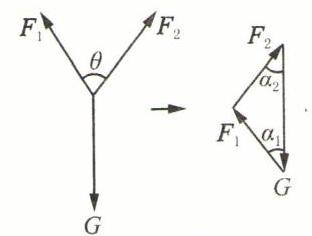
\includegraphics[width=0.2\textwidth]{bodyxb/src/bo_d20cdrf7aajc73bfmvhg_16_1215_1369_312_236_0.jpg}
\end{center}


(第 191 题)

$\therefore \;{\alpha }_{1} = {\alpha }_{2} = \dfrac{1}{2}\theta .\left| {\mathbf{F}}_{1}\right| \cos {\alpha }_{1} + \left| {\mathbf{F}}_{2}\right| \cos {\alpha }_{2} = 2\left| \mathbf{F}\right| \cos \dfrac{1}{2}\theta  = \left| \mathbf{G}\right|$ ,

$\therefore \;\left| \mathbf{F}\right|  = \dfrac{\left| \mathbf{G}\right| }{2\cos \dfrac{1}{2}\theta }$ .

192. $\left( {\dfrac{21}{2},{10}}\right) ,\left( {4, - 3}\right)$ 提示: 记 $\vv{AB} = \vv{a},\vv{AD} = \vv{b},C\left( {{x}_{1},{y}_{1}}\right) ,D\left( {{x}_{2},{y}_{2}}\right)$ .

$\therefore \vv{AM} = \dfrac{1}{2}\vv{AC} = \dfrac{1}{2}\left( {\vv{AB} + \vv{BC}}\right)  = \dfrac{1}{2}\left( {\vv{AB} + \vv{AD}}\right)  = \dfrac{1}{2}\left( {\vv{a} + \vv{b}}\right)$ .

已知 $\vv{AB} = \left( {2,6}\right)  - \left( {-\dfrac{9}{2}, - 7}\right)  = \left( {\dfrac{13}{2},{13}}\right)  = \vv{a},\vv{AM} = \left( {3,\dfrac{3}{2}}\right)  - \left( {-\dfrac{9}{2}, - 7}\right)  = \left( {\dfrac{15}{2},\dfrac{17}{2}}\right)$

$\therefore \vv{b} = 2\vv{AM} - \vv{AB} = 2 \cdot  \left( {\dfrac{15}{2},\dfrac{17}{2}}\right)  - \left( {\dfrac{13}{2},{13}}\right)  = \left( {\dfrac{17}{2},4}\right)$ . 又 $\because \vv{AD} = \left( {{x}_{2},{y}_{2}}\right)  - \left( {-\dfrac{9}{2}, - 7}\right)  = \vv{b} = \left( {\dfrac{17}{2},4}\right)$ ,

$\therefore \;\left( {{x}_{2},{y}_{2}}\right)  = \left( {4, - 3}\right) .\vv{DC} = \left( {{x}_{1},{y}_{1}}\right)  - \left( {4, - 3}\right)  = \vv{AB} = \vv{a} = \left( {\dfrac{13}{2},{13}}\right)$ ,

$\therefore \;\left( {{x}_{1},{y}_{1}}\right)  = \left( {\dfrac{21}{2},{10}}\right) ,\;\therefore \;C\left( {\dfrac{21}{2},{10}}\right) ,D\left( {4, - 3}\right) .$

193. $5\sqrt{13}$ 提示:设点 $C$ 的坐标为 $C\left( {x,y}\right)$ ,有 $\dfrac{1}{3}\left\lbrack  {\left( {0,7}\right)  + \left( {-4,5}\right)  + \left( {x,y}\right) }\right\rbrack   = \left( {0,\dfrac{1}{3}}\right) ,\therefore \left( {x,y}\right)  = \left( {4, - {11}}\right)$ ,点 $D$ 的坐标为 $\dfrac{1}{2}\left\lbrack  {\left( {0,7}\right)  + \left( {-{4.5}}\right) }\right\rbrack   = \left( {-2,6}\right)$ .

$\therefore \;\vv{CD} = \left( {-2,6}\right)  - \left( {4, - {11}}\right)  = \left( {-6,{17}}\right) ,\;\therefore \;\left| \vv{CD}\right|  = \sqrt{{\left( -6\right) }^{2} + {17}^{2}} = 5\sqrt{13}$ .

194. 东南风, $\sqrt{2}v$ 提示:如图, ${v}_{\text{ 风 }} = {v}_{\text{ 相 }} + {v}_{\text{ 人 }},{v}_{\text{ 风 }},{v}_{\text{ 相 }},{v}_{\text{ 人 }}$ 分别是上述设定下的绝对速度,相对速度和牵连速度, $\therefore {v}_{\text{ 相 }} = {v}_{\text{ 风 }} - {v}_{\text{ 人 }}$ . 易得 $\left| {v}_{\text{ 相 }}\right|  = \sqrt{{v}^{2} + {v}^{2}}\mathrm{\;{km}}/\mathrm{h} = \sqrt{2}v\mathrm{\;{km}}/\mathrm{h}$ . 风自东南吹向西北,

\begin{center}
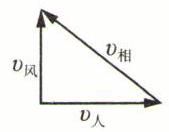
\includegraphics[width=0.2\textwidth]{bodyxb/src/bo_d20cdrf7aajc73bfmvhg_17_1231_182_169_132_0.jpg}
\end{center}


(第 194 题)

$\therefore$ 此人感到的风向为东南风,风速为 $\sqrt{2}v\mathrm{\;{km}}/\mathrm{h}$ .

195. ${20.8}\mathrm{\;N}$ 提示:如图, $\theta  = \dfrac{1}{2} \cdot  {60}^{ \circ  } = {30}^{ \circ  },\left| {\mathbf{F}}_{\text{ 合 }}\right|  = 2\left| \mathbf{F}\right| \cos \theta  = \sqrt{3}\left| \mathbf{F}\right|  = {12}\sqrt{3}\mathrm{\;N},\left| {\mathbf{F}}_{\text{ 合 }}\right|  \approx  {20.8}\mathrm{\;N}$ .

\begin{center}
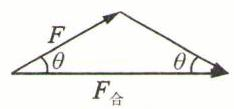
\includegraphics[width=0.2\textwidth]{bodyxb/src/bo_d20cdrf7aajc73bfmvhg_17_335_501_234_109_0.jpg}
\end{center}


(第 195 题)

\begin{center}
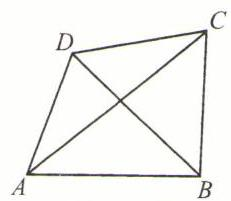
\includegraphics[width=0.2\textwidth]{bodyxb/src/bo_d20cdrf7aajc73bfmvhg_17_677_408_231_201_0.jpg}
\end{center}


(第 196 题)

196. 如图,在四边形 ${ABCD}$ 中, $\because A{B}^{2} + D{C}^{2} = A{D}^{2} + B{C}^{2}$ ,

$\therefore \vv{A{B}^{2}} + \vv{D{C}^{2}} = \vv{A{D}^{2}} + \vv{B{C}^{2}},\;\therefore \;\vv{A{B}^{2}} - \vv{B{C}^{2}} = \vv{A{D}^{2}} - \vv{D{C}^{2}}$ ,

即 $\left( {\vv{AB} + \vv{BC}}\right)  \cdot  \left( {\vv{AB} - \vv{BC}}\right)  = \left( {\vv{AD} + \vv{DC}}\right)  \cdot  \left( {\vv{AD} - \vv{DC}}\right)$ .

$\therefore \vv{AC} \cdot  \left( {\vv{AB} - \vv{BC}}\right)  = \vv{AC} \cdot  \left( {\vv{AD} - \vv{DC}}\right)$ ,

\begin{center}
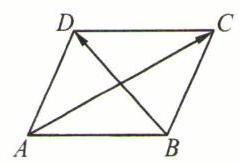
\includegraphics[width=0.2\textwidth]{bodyxb/src/bo_d20cdrf7aajc73bfmvhg_17_1161_784_239_164_0.jpg}
\end{center}


(第 197 题)

$\therefore \vv{AC} \cdot  \left( {\vv{AB} - \vv{BC} - \vv{AD} + \vv{DC}}\right)  = 0$ . 化简,得 $\vv{AC} \cdot  2\vv{DB} = 0$ ,即 $\vv{AC} \cdot  \vv{DB} = 0$ ,

$\therefore \vv{AC}\bot \vv{DB}$ ,

$\therefore {AC} \bot  {DB}$ . 所以对边平方和相等的四边形的对角线互相垂直.

197. 如图, $A{C}^{2} + B{D}^{2} = \vv{A{C}^{2}} + \vv{B{D}^{2}} = {\left( \vv{AB} + \vv{AD}\right) }^{2} + {\left( \vv{AD} - \vv{AB}\right) }^{2}$

$= {\vv{AB}}^{2} + 2\vv{AB} \cdot  \vv{AD} + {\vv{AD}}^{2} + {\vv{AD}}^{2} - 2\vv{AD} \cdot  \vv{AB} + {\vv{AB}}^{2}$

$= 2\left( {{\vv{AB}}^{2} + {\vv{AD}}^{2}}\right)  = 2\left( {A{B}^{2} + A{D}^{2}}\right) .$

\begin{center}
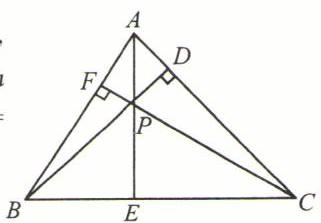
\includegraphics[width=0.2\textwidth]{bodyxb/src/bo_d20cdrf7aajc73bfmvhg_17_1104_1035_321_223_0.jpg}
\end{center}


(第 198 题)

198. 如图,在 $\bigtriangleup {ABC}$ 中, ${BD}$ , ${CF}$ 分别是边 ${AC}$ , ${AB}$ 上的高,且 ${BD}$ , ${CF}$ 交于点 $P$ . 设 $\vv{PA} = a$ , $\vv{PB} = b,\vv{PC} = c$ ,则 $\vv{AB} = b - a,\vv{BC} = c - b,\vv{CA} = a - c.\;\because \;\vv{PA}\bot \vv{BC},\vv{PC}\bot \vv{AB},\;\therefore \;a$  $\cdot  \left( {c - b}\right)  = 0$ ,且 $c \cdot  \left( {b - a}\right)  = 0$ ,即 $a \cdot  c - a \cdot  b = 0$ ,且 $c \cdot  b - c \cdot  a = 0$ , $\therefore c \cdot  b - a \cdot  b =$ 0,因此, $b \cdot  \left( {c - a}\right)  = 0$ ,即 $\vv{PB} \cdot  \vv{CA} = 0.\;\therefore \;$ 即 $\vv{PB}\bot \vv{CA},\;\therefore \;{PB}\bot {AC}$ . 故 $P$ 是 $\bigtriangleup {ABC}$ 的三条高线的交点.

199. 如图,平衡时两根绳子拉力分别为 ${\mathbf{F}}_{1},{\mathbf{F}}_{2}$ . 由题意可知, $\left| {{\mathbf{F}}_{1} + {\mathbf{F}}_{2}}\right|  = {400}$ .

由于两根绳子与铅垂线的夹角分别是 ${30}^{ \circ  },{60}^{ \circ  }$ ,因此, ${\mathbf{F}}_{1}$ 的大小为 ${400} \times  \cos {30}^{ \circ  } = {200}\sqrt{3}\left( \mathrm{\;N}\right) ,{\mathbf{F}}_{2}$ 的大小为 ${400} \times  \cos {60}^{ \circ  } = {200}\left( \mathrm{\;N}\right)$ . 所以两根绳子拉力的大小分别为 ${200}\sqrt{3}\mathrm{\;N},{200}\mathrm{\;N}$ .

\begin{center}
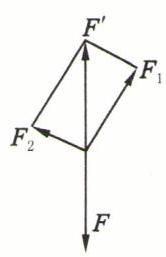
\includegraphics[width=0.2\textwidth]{bodyxb/src/bo_d20cdrf7aajc73bfmvhg_17_1239_1296_166_257_0.jpg}
\end{center}


(第 199 题)

200. 方法一:如图,由三角形知识可知,无论小船渡河的合速度方向偏向下游哪一方向,欲使小船划行速度最小,划行方向都应与合速度方向垂直. 由图直观可看出,当合速度方向恰指向瀑布所在的对岸点 $B$ 时, 小船划行速度最小.

设码头 $A$ 到瀑布的水平距离为 $s$ ,则 $\dfrac{{v}_{\text{ 船 }}}{{v}_{\text{ 水 }}} = \dfrac{L}{\sqrt{{s}^{2} + {L}^{2}}}$ .

代入得 ${v}_{\text{ 船 }} = \dfrac{3}{5}{v}_{ \star  } = 3\mathrm{\;m}/\mathrm{s}$ ,此时,在直角三角形中水流的相反方向与船的行驶方向的夹角为 $\gamma$ ,因此, $\cos \gamma  \approx  \dfrac{3}{5}$ .

故船的行驶方向与水流方向的夹角为 ${180}^{ \circ  } - {53}^{ \circ  } = {127}^{ \circ  }$ .

\begin{center}
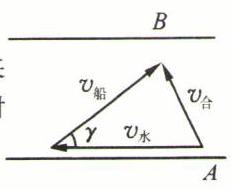
\includegraphics[width=0.2\textwidth]{bodyxb/src/bo_d20cdrf7aajc73bfmvhg_17_1194_1717_231_189_0.jpg}
\end{center}


(第 200 题)

方法二: 以点 $A$ 为原点,水流方向为 $x$ 轴,垂直河岸方向为 $y$ 轴. 设小船划行方向与水流方向的夹角为 $\theta$ ,则小船沿 $x$ 轴方向的速度 ${v}_{x} = {v}_{水} + {v}_{\text{ 船 }}\cos \theta$ ,沿 $y$ 轴方向的速度 ${v}_{y} = {v}_{\text{ 船 }}\sin \theta$ ,到达对岸时 ${s}_{y} = {v}_{y}t = L = {60},{s}_{x} = {v}_{x}t.$

欲不下滑到瀑布,应有 ${s}_{x} \leq  s = {80}\mathrm{\;m}$ .

由以上各式得 $\left( {{v}_{水} + {v}_{\text{ 船 }}\cos \theta }\right)  \cdot  \dfrac{L}{{v}_{\text{ 船 }}\sin \theta } \leq  s = {80}$ .

整理,得 ${v}_{\text{ 船 }} \geq  \dfrac{{v}_{ 水 }L}{s\sin \theta  - L\cos \theta }$ . 令 $\tan \theta  = \dfrac{L}{s} = \dfrac{3}{4}$ ,得 ${v}_{\text{ 船 }} \geq  \dfrac{{v}_{ \star  }L}{\sqrt{{s}^{2} + {L}^{2}}\sin \left( {\theta  - \varphi }\right) }$ .

由此可得出 $\theta  - \varphi  = {90}^{ \circ  }$ 时, ${v}_{\text{ 船 }}$ 有最小值,此时, $\tan \varphi  = \dfrac{3}{4},{v}_{\text{ 船min }} = \dfrac{{v}_{ * }L}{\sqrt{{s}^{2} + {L}^{2}}} = 3\left( {\mathrm{\;m}/\mathrm{s}}\right)$ . 与水流方向的夹角为 $\theta  = {90}^{ \circ  } + \varphi  \approx  {127}^{ \circ  }$ .

201. B 提示: $\left| {AB}\right|  = \sqrt{{\left( \cos 2\alpha  - \cos \alpha \right) }^{2} + {\left( \sin 2\alpha  - \sin \alpha \right) }^{2}} = \sqrt{2 - 2\left( {\cos {2\alpha }\cos \alpha  + \sin {2\alpha }\sin \alpha }\right) } = \sqrt{2 - 2\cos \left( {{2\alpha } - \alpha }\right) } =$  $\sqrt{4 \cdot  \dfrac{1 - \cos \alpha }{2}} = 2\left| {\sin \dfrac{\alpha }{2}}\right| .$

202. $D$ 提示: 设点 $M$ 的坐标是(x,0),由题意 $\sqrt{{x}^{2}} = \sqrt{{\left( x - 5\right) }^{2} + {3}^{2}}$ ,整理得 ${10x} = {34},\therefore x = \dfrac{17}{5}$ ,

$\therefore$ 点 $M$ 的坐标是(3.4,0).

203. B 提示: $\left| {PQ}\right|  = \sqrt{{\left( \cos \beta  - \cos \alpha \right) }^{2} + {\left( \sin \beta  - \sin \alpha \right) }^{2}} = \sqrt{2 - 2\left( {\cos \beta \cos \alpha  + \sin \beta \sin \alpha }\right) } = \sqrt{2 - 2\cos \left( {\beta  - \alpha }\right) } \leq  \sqrt{2 + 2} = 2$ , $\beta  - \alpha  = \pi  + {2k\pi }\left( {k \in  \mathbf{Z}}\right)$ 时, $\left| {PQ}\right|$ 取得最大值 2.

204. D 提示: 对于选项 $A : \lambda  \leq  0$ 也是可能的,例如点 $P$ 在 ${P}_{1}{P}_{2}$ 的延长线上时, $\lambda$ 即小于 0,故错误.

对于选项 B: 点 $P$ 在 ${P}_{2}{P}_{1}$ 的延长线上时, $\lambda$ 也小于 0,错误.

对于选项 ${C}_{1}\lambda  =  - 1$ 时, $\vv{{P}_{1}P} =  - \vv{P{P}_{2}}$ ,故 $\vv{{P}_{1}P} + \vv{P{P}_{2}} = 0$ . 因此 $\vv{{P}_{1}{P}_{2}} = \mathbf{0}$ ,当 ${P}_{1},{P}_{2}$ 重合时,任取点 $P$ (可以不与 ${P}_{1},{P}_{2}$ 重合),都能使 $\lambda  =  - 1$ ,错误. 对于选项 $D : \lambda  = 0$ 时, $\vv{{P}_{1}P} = \mathbf{0}$ ,故点 $P$ 与 ${P}_{1}$ 重合,正确. 205. C 提示: 即 $\vv{AP} = \dfrac{1}{3}\vv{PB},\therefore \vv{AP} + \vv{PB} = \vv{AB} = \dfrac{1}{3}\vv{PB} + \vv{PB} = \dfrac{4}{3}\vv{PB},\therefore \vv{AB} =  - \dfrac{4}{3}\vv{BP}$ . 206. A 提示: 点 $C$ 的坐标为 $\left( {\dfrac{m + \left( {-2}\right)  \cdot  \left( {-m}\right) }{1 + \left( {-2}\right) },\dfrac{-n + \left( {-2}\right)  \cdot  n}{1 + \left( {-2}\right) }}\right)$ ,即(-3m,3n). 207. A 提示: $\dfrac{\left| \vv{PA}\right| }{\left| \vv{AQ}\right| } = \dfrac{\left| PA\right| }{\left| {PA}\right|  + \left| {PQ}\right| } = \dfrac{\dfrac{1}{3}\left| {PQ}\right| }{\dfrac{1}{3}\left| {PQ}\right|  + \left| {PQ}\right| } = \dfrac{1}{4},\;\therefore \;\vv{PA} =  - \dfrac{1}{4}\vv{AQ},\;\therefore \;$ 点 $A$ 的坐标为 $\left( {\dfrac{-1 - \dfrac{1}{4} \cdot  3}{1 - \dfrac{1}{4}},\dfrac{-6 - \dfrac{1}{4} \cdot  0}{1 - \dfrac{1}{4}}}\right)$ ,即 $\left( {-\dfrac{7}{3}, - 8}\right)$ . 208. $C$ 提示: 点 $M$ 的横坐标为 $\dfrac{4 - {2\lambda }}{1 + \lambda } = 0.\;\therefore \;\lambda  = 2$ . 209. B 提示: 由题意, $\vv{AC} = \vv{AB} + \vv{BC} = \dfrac{1}{2}\vv{BC},\therefore \vv{CB} = 2\vv{CA}$ . 210. B 提示: 设点 $C$ 的坐标为 $C\left( {x,y}\right)$ ,可以得到 $\left\{  \begin{array}{l} \dfrac{2 + 8 + x}{3} = 2, \\  \dfrac{3 - 4 + y}{3} =  - 1, \end{array}\right.$ 解得 $\left\{  \begin{array}{l} x =  - 4, \\  y =  - 2. \end{array}\right.$  $\therefore$ 点 $C$ 的坐标为 $C\left( {-4, - 2}\right)$ . 211. (1) 5 或 -3 提示: 由题意 $\sqrt{{\left( x - 1\right) }^{2} + {\left( 2 - 5\right) }^{2}} = 5,\therefore {\left( x - 1\right) }^{2} = {4}^{2},\therefore$ 点 $B$ 的横坐标是 $x = 5$ 或 $x =  - 3$ . (2) $M\left( {0, - \dfrac{1}{2}}\right)$ 提示:设点 $M$ 的坐标为(0, y),由题意得 $\sqrt{{4}^{2} + {\left( y + 1\right) }^{2}} = \sqrt{{2}^{2} + {\left( y - 3\right) }^{2}}$ ,整理得 ${8y} =  - 4$ , $\therefore y =  - \dfrac{1}{2},\;\therefore \;$ 点 $M$ 的坐标是 $M\left( {0, - \dfrac{1}{2}}\right)$ . (3) $Q\left( {3,5}\right)$ 或 $Q\left( {-{17},{145}}\right)$ 提示:设点 $Q$ 的坐标为(x, y),由题意有 $\sqrt{{x}^{2} + {\left( y - 1\right) }^{2}} = \sqrt{{\left( x - 7\right) }^{2} + {\left( y - 2\right) }^{2}} = \left| y\right|$ . 由 $\sqrt{{x}^{2} + {\left( y - 1\right) }^{2}} = \sqrt{{\left( x - 7\right) }^{2} + {\left( y - 2\right) }^{2}}$ ,整理得 ${7x} + y - {26} = 0$ . 由 $\sqrt{{x}^{2} + {\left( y - 1\right) }^{2}} = \left| y\right|$ ,整理得 $y = \dfrac{1}{2}\left( {{x}^{2} + }\right.$ 1). 代入 $y = {26} - {7x}$ ,整理得 ${x}^{2} + {14x} - {51} = 0,\therefore {x}_{1} = 3,{x}_{2} =  - {17}$ ,对应地 ${y}_{1} = 5,{y}_{2} = {145}$ ,

$\therefore$ 点 $Q$ 的坐标是 $Q\left( {3,5}\right)$ 或 $Q\left( {-{17},{145}}\right)$ .

212. (1) 3 提示: 设 $\vv{AP} = \lambda \vv{PB}$ ,则有 $\left\{  \begin{array}{l} x = \dfrac{2 + {5\lambda }}{1 + \lambda }, \\  1 = \dfrac{-4 + {11\lambda }}{1 + \lambda }, \end{array}\right.$ 解得 $\left\{  \begin{array}{l} \lambda  = \dfrac{1}{2}, \\  x = 3. \end{array}\right.$

(2) $\left( {6,0}\right) ,\left( {0,3}\right)$ 提示: 设直线 ${AB}$ 与 $x$ 轴, $y$ 轴交点的坐标分别为 $P\left( {x,0}\right) ,Q\left( {0,y}\right)$ ,若 $\vv{AP} = {\lambda }_{1}\vv{PB}$ ,则有 $\left\{  {\begin{array}{l} \dfrac{4 - 2{\lambda }_{1}}{1 + {\lambda }_{1}} = x, \\  \dfrac{1 + 4{\lambda }_{1}}{1 + {\lambda }_{1}} = 0, \end{array}\text{ 解得 }\left\{  {\begin{array}{l} {\lambda }_{1} =  - \dfrac{1}{4}, \\  x = 6. \end{array}\text{ 若 }\vv{AQ} = {\lambda }_{2}\vv{QB}\text{ ,则有 }\left\{  {\begin{array}{l} \dfrac{4 - 2{\lambda }_{2}}{1 + {\lambda }_{2}} = 0, \\  \dfrac{1 + 4{\lambda }_{2}}{1 + {\lambda }_{2}} = y, \end{array}\text{ 解得 }\left\{  {\begin{array}{l} {\lambda }_{2} = 2, \\  y = 3. \end{array}\;\therefore \;\text{ 直线 }{AB}\text{ 与 }x\text{ 轴交点的坐标是 }}\right. }\right. }\right. }\right.$ (6,0),与 $y$ 轴交点的坐标是(0,3)

(3) $\dfrac{1}{2}$ 提示:由题意, $\vv{{P}_{3}{P}_{2}} =  - \dfrac{3}{2}\vv{{P}_{1}{P}_{3}}$ ,

$\therefore \vv{{P}_{1}{P}_{2}} = \vv{{P}_{1}{P}_{3}} + \vv{{P}_{3}{P}_{2}} = \left( {1 - \dfrac{3}{2}}\right) \vv{{P}_{1}{P}_{3}} =  - \dfrac{1}{2}\vv{{P}_{1}{P}_{3}} = \dfrac{1}{2}\vv{{P}_{3}{P}_{1}},\;\therefore \;t = \dfrac{1}{2}$ .

(4) $\lambda  = 4,x =  - 4$ 提示: 由题意有 $\left\{  \begin{array}{l} \dfrac{4 - {6\lambda }}{1 + \lambda } = x, \\  \dfrac{2 - {4\lambda }}{1 + \lambda } =  - 2\dfrac{4}{5}, \end{array}\right.$ 解得 $\left\{  \begin{array}{l} \lambda  = 4, \\  x =  - 4. \end{array}\right.$

(5) $\left( {\dfrac{1}{3},0}\right)$ 或(-5,8)提示:情况一: $\vv{PA} = 2\vv{PB},\therefore \vv{AP} =  - 2\vv{PB}$ . 点 $P$ 的坐标为

$\left( {\dfrac{3 + \left( {-2}\right)  \cdot  \left( {-1}\right) }{1 - 2},\dfrac{-4 + \left( {-2}\right)  \cdot  2}{1 - 2}}\right)$ ,即 $P\left( {-5,8}\right)$

情况二: $\vv{PA} = 2\vv{BP},\therefore \vv{AP} = 2\vv{PB}$ . 点 $P$ 的坐标 $\left( {\dfrac{3 + 2\left( {-1}\right) }{1 + 2},\dfrac{-4 + 2 \cdot  2}{1 + 2}}\right)$ ,即 $P\left( {\dfrac{1}{3},0}\right)$ . 综上,点 $P$ 的坐标是 $P\left( {-5,8}\right)$ 或 $P\left( {\dfrac{1}{3},0}\right)$ (6) $\text{ ① }\lambda  \in  \left( {0, + \infty }\right)$ ② $\lambda  \in  \left( {-\infty , - 1}\right)$ 提示: 设此时 $\vv{{P}_{1}{P}_{2}} = {\lambda }^{\prime }\vv{{P}_{2}P}$ ,点 ${P}_{2}$ 在线段 ${P}_{1}P$ 内, ${\lambda }^{\prime } \in  \left( {0, + \infty }\right)$ . $\therefore \vv{{P}_{1}P} = \vv{{P}_{1}{P}_{2}} + \vv{{P}_{2}P} = \left( {{\lambda }^{\prime } + 1}\right) \vv{{P}_{2}P},\;\therefore \;\lambda  =  - \left( {1 + {\lambda }^{\prime }}\right) ,\;\therefore \;\lambda  \in  \left( {-\infty , - 1}\right)$ . ③ $\lambda  \in  \left( {-1,0}\right)$ 提示: 设此时 $\vv{{P}_{2}{P}_{1}} = {\lambda }^{\prime }\vv{{P}_{1}P},{P}_{1}$ 在线段 ${P}_{2}P$ 内, ${\lambda }^{\prime } \in  \left( {0, + \infty }\right)$ . $\therefore \vv{{P}_{2}P} = \vv{{P}_{2}{P}_{1}} + \vv{{P}_{1}P} = \left( {{\lambda }^{\prime } + 1}\right) \vv{{P}_{1}P},\;\therefore \lambda  =  - \dfrac{1}{1 + {\lambda }^{\prime }},\;\therefore \lambda  \in  \left( {-1,0}\right)$ . 213. (1) 情况一: 若 $\vv{BC} = 2\vv{AC}$ ,则 $\vv{BC} =  - 2\vv{CA}$ . 考察点 $C$ 的坐标 $\left\{  \begin{array}{l} 1 = \dfrac{-2 - {2x}}{1 - 2}, \\  1 = \dfrac{y - {10}}{1 - 2}, \end{array}\right.$ 解得 $\left\{  \begin{array}{l} x =  - \dfrac{1}{2}, \\  y = 9. \end{array}\right.$ 情况二: 若 $\vv{BC} = 2\vv{CA}$ ,则考察点 $C$ 的坐标 $\left\{  \begin{array}{l} 1 = \dfrac{-2 + {2x}}{1 + 2}, \\  1 = \dfrac{y + {10}}{1 + 2}, \end{array}\right.$ 解得 $\left\{  \begin{array}{l} x = \dfrac{5}{2}, \\  y =  - 7. \end{array}\right.$ (2)设顶点 $B,C$ 的坐标分别为 $B\left( {{x}_{2},{y}_{2}}\right) ,C\left( {{x}_{3},{y}_{3}}\right)$ . 根据中点及重心的性质,有 $\left\{  \begin{array}{l} 2 = \dfrac{3 + {x}_{2}}{2} \\  4 = \dfrac{1 + {y}_{2}}{2} \end{array}\right.$ ,解得 $\left\{  {\begin{array}{l} {x}_{2} = 1, \\  {y}_{2} = 7. \end{array}\;\therefore \;B(1}\right.$ , 7), $\left\{  \begin{array}{l} 3 = \dfrac{3 + 1 + {x}_{3}}{3}, \\  4 = \dfrac{1 + 7 + {y}_{3}}{3}, \end{array}\right.$ 解得 $\left\{  \begin{array}{l} {x}_{3} = 5, \\  {y}_{3} = 4. \end{array}\right.$  $\therefore$ 顶点 $B,C$ 的坐标分别为 $B\left( {1,7}\right) ,C\left( {5,4}\right)$ . 214. (1) 设点 $C$ 的坐标为(x, y),则 $\vv{BA} = \left( {1,0}\right)  - \left( {3,1}\right)  = \left( {-2, - 1}\right) ,\left| \vv{BA}\right|  = \sqrt{{2}^{2} + {1}^{2}} = \sqrt{5},\vv{BC} = \left( {x,y}\right)  - \left( {3,1}\right)  = (x -$  $3,y - 1),\left| \vv{BC}\right|  = \sqrt{{\left( x - 3\right) }^{2} + {\left( y - 1\right) }^{2}} \cdot  \angle {ABC} = {90}^{ \circ  } \Leftrightarrow  \vv{BA} \cdot  \vv{BC} = 0$ ,

$\therefore \left\{  \begin{array}{l}  - 2\left( {x - 3}\right)  - \left( {y - 1}\right)  = 0, \\  \sqrt{5} = \sqrt{{\left( x - 3\right) }^{2} + {\left( y - 1\right) }^{2}}. \end{array}\right.$ 解得 $\left\{  \begin{array}{l} x = 4, \\  y =  - 1 \end{array}\right.$ 或 $\left\{  \begin{array}{l} x = 2, \\  y = 3. \end{array}\right.$

$\therefore$ 顶点 $C$ 的坐标为 $C\left( {4, - 1}\right)$ 或 $C\left( {2,3}\right)$ .

(2)设 ${AC},{BD}$ 交于点 $M\left( {x,0}\right)$ . 根据矩形对角线的性质, $\left| \vv{MA}\right|  = \left| \vv{MB}\right| ,\;\therefore \;\sqrt{{\left( x + 1\right) }^{2} + {3}^{2}} = \sqrt{{\left( x + 2\right) }^{2} + {4}^{2}}$ , $x =  - 5,\therefore$ 交点坐标为(-5,0). 根据矩形对角线性质, $M$ 为 ${AC},{BD}$ 的中点,设点 $C,D$ 的坐标分别为 $\left( {x}_{3}\right.$ ,

$\left. {{y}_{3}),D\left( {{x}_{4},{y}_{4}}\right) ,\;\therefore \left\{  \begin{array}{l} \dfrac{-1 + {x}_{3}}{2} =  - 5, \\  3 + {y}_{3} = 0, \end{array}\right. \text{ 解得 }\left\{  \begin{array}{l} {x}_{3} =  - 9, \\  {y}_{3} =  - 3. \end{array}\right. }\right)$

$\therefore \left\{  {\begin{array}{l} \dfrac{-2 + {x}_{4}}{2} =  - 5, \\  \dfrac{4 + {y}_{4}}{2} = 0, \end{array}\text{ 解得 }\left\{  {\begin{array}{l} {x}_{4} =  - 8, \\  {y}_{4} =  - 4. \end{array}\;\therefore \;\text{ 顶点 }C,D\text{ 的坐标为 }C\left( {-9, - 3}\right) ,D\left( {-8, - 4}\right) .}\right. }\right.$

215. B 提示: 易知: $\vv{BD} = \dfrac{1}{3}\vv{BC},\therefore \vv{BD} = \dfrac{1}{2}\vv{DC}$ ,由定比分点公式可知: $D\left( {\dfrac{-4 + \dfrac{1}{2} \cdot  5}{1 + \dfrac{1}{2}},\dfrac{0 + \dfrac{1}{2} \cdot  \left( {-3}\right) }{1 + \dfrac{1}{2}}}\right)$ .

$\therefore$ 点 $D$ 的坐标为 $D\left( {-1, - 1}\right)$ .

216. $C$ 提示: 方法一: 以点 $A$ 为坐标原点, $\vv{AB},\vv{AD}$ 分别为 $x,y$ 轴正方向建立平面直角坐标系,并设点 $E$ 的坐标 $E\left( {x,0}\right)$ , 易知 $M\left( {2,1}\right) ,\therefore \vv{EM} = \left( {2,1}\right)  - \left( {x,0}\right)  = \left( {2 - x,1}\right) .\because \left| \vv{EM}\right|  = \left| \vv{EA}\right| ,\therefore \sqrt{{\left( 2 - x\right) }^{2} + {1}^{2}} = x,\therefore {x}^{2} -$  ${4x} + 5 = {x}^{2},\;\therefore \;x = \dfrac{5}{4},\;\therefore \;\left| \vv{EM}\right|  = \left| \vv{EA}\right|  = \dfrac{5}{4}.$

方法二: 设 ${AE} = x$ ,则 ${EB} = 2 - x,{EM} = {EA} = x,{MB} = \dfrac{1}{2}{BC} = 1$ . 在 $\bigtriangleup {EMB}$ 中, $\angle B = {90}^{ \circ  }$ ,运用勾股定理,得 ${\left( 2 - x\right) }^{2} +$  ${1}^{2} = {x}^{2},\;\therefore \;x = \dfrac{5}{4}.$

217. C 提示: 记 ${BC}$ 的中点为 $M$ ,根据重心的性质, ${AG} = \dfrac{2}{3}{AM}$ . 作为特例,当 ${PQ}//{BC}$ 时, $\dfrac{AQ}{AB} = \dfrac{AP}{AC} = \dfrac{AG}{AM} = \dfrac{2}{3}$ ,此时, $m =$  $n = \dfrac{3}{2},m + n = 3$ . 下面证明这一结论具有一般性,记 $\vv{AB} = \vv{a},\vv{AC} = \vv{b},\;\therefore \;\vv{BC} = \vv{AC} - \vv{AB} = \vv{b} - \mathbf{c}$ ,

$\therefore \vv{AM} = \vv{AB} + \vv{BM} = \vv{AB} + \dfrac{1}{2}\left( \vv{BC}\right)  = \dfrac{1}{2}\left( {b + c}\right)$

$\because A,G,M$ 三点共线, $\therefore$ 存在唯一的 $k$ ,使 $\vv{AG} = k\vv{AM}$ ,而 $\left| \vv{AG}\right|  = k\left| \vv{AM}\right| ,\therefore k = \dfrac{\left| \vv{AG}\right| }{\left| \vv{AM}\right| } = \dfrac{2}{3},\therefore \vv{AG} = \dfrac{2}{3}$

\begin{itemize}
\item $\dfrac{1}{2}\left( {b + c}\right)  = \dfrac{1}{3}\left( {b + c}\right) ,\vv{QG} = \vv{AG} - \vv{AQ} = \dfrac{1}{3}\left( {b + c}\right)  - \dfrac{1}{m}c = \dfrac{1}{3}b + \left( {\dfrac{1}{3} - \dfrac{1}{m}}\right) c,\vv{GP} = \vv{AP} - \vv{AG} = \dfrac{1}{n}b - \dfrac{1}{3}\left( {b + c}\right)  =$  $\left( {\dfrac{1}{n} - \dfrac{1}{3}}\right) b - \dfrac{1}{3}c.\because Q,G,P$ 三点共线, $\therefore$ 存在唯一的 $\mu$ ,使 $\vv{QG} = \mu \vv{GP}.\because b,c$ 不共线,
\end{itemize}

$\therefore \left\{  \begin{array}{l} \dfrac{1}{3} = \mu \left( {\dfrac{1}{n} - \dfrac{1}{3}}\right) , \\  \dfrac{1}{3} - \dfrac{1}{m} =  - \dfrac{1}{3}\mu . \end{array}\right.$ 消去 $\mu$ ,有 $\left( {\dfrac{1}{m} - \dfrac{1}{3}}\right) \left( {\dfrac{1}{n} - \dfrac{1}{3}}\right)  = \dfrac{1}{3} \cdot  \dfrac{1}{3},\therefore \dfrac{m + n - 3}{mn} = 0.m,n \neq  0,\therefore m + n = 3$ .

218. $C$ 提示: 如图,分力 ${\mathbf{F}}_{1},{\mathbf{F}}_{2}$ 在合力 $\mathbf{F}$ 的异侧 (否则 $\theta  \neq  0$ 时, ${\mathbf{F}}_{1},{\mathbf{F}}_{2},\mathbf{F}$ 将共线),容易看出 $\left| \mathbf{F}\right|  = 2\left| {\mathbf{F}}_{1}\right| \cos \theta  =$  $2\left| {\mathbf{F}}_{2}\right| \cos \theta .\left| {\mathbf{F}}_{1}\right|  = \left| {\mathbf{F}}_{2}\right|  = \dfrac{\left| \mathbf{F}\right| }{2\cos \theta },\theta  \in  \left( {0,\dfrac{\pi }{2}}\right) .\;{\mathbf{F}}_{1}$ 与 ${\mathbf{F}}_{2}$ 的夹角是 $\alpha  = {2\theta },\alpha  \in  \left( {0,\pi }\right) .$

$\therefore$ 当 $\alpha$ 增大时, $\theta$ 增大, $\left| {\mathbf{F}}_{1}\right|  = \left| {\mathbf{F}}_{2}\right|$ 越来越大.

\begin{center}
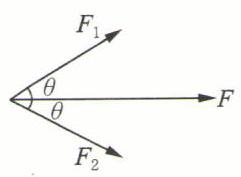
\includegraphics[width=0.2\textwidth]{bodyxb/src/bo_d20cdrf7aajc73bfmvhg_20_503_1428_241_177_0.jpg}
\end{center}


(第 218 题)

\begin{center}
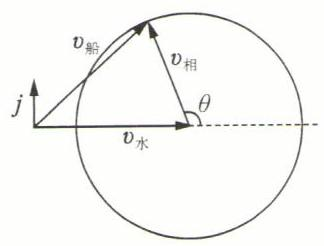
\includegraphics[width=0.2\textwidth]{bodyxb/src/bo_d20cdrf7aajc73bfmvhg_20_827_1355_324_246_0.jpg}
\end{center}


(第 219 题)

219. D 提示:取地面为静止参照系,河水为运动参照系,考查船的运动: ${v}_{\text{ 船 }} = {v}_{\text{ 相 }} + {v}_{\text{ 水 }}$ . ${v}_{\text{ 船 }}$ 是船相对地面的绝对速度, ${v}_{\text{ 相 }}$ 是船相对水流的航行速度, $\left| {v}_{\text{ 相 }}\right|  = 3\mathrm{\;m}/\mathrm{s},{v}_{\text{ 水 }}$ 是牵连速度, $\left| {v}_{\text{ 水 }}\right|  = 4\mathrm{\;m}/\mathrm{s}$ . 如图, ${v}_{\text{ 船 }}$ 的轨迹是一个圆 (或考虑实际情况只取上半圆). 现考虑 4 个选项:对于选项 ${A}_{:}{v}_{\text{ 船 }}$ 不可能与 ${v}_{\text{ 水 }}$ 垂直,错误. 对于选项 ${B}_{:}\left| {v}_{\text{ 船 }}\right|  = \left| {{v}_{\text{ 相 }} + {v}_{\text{ 水 }}}\right|  \in  \left\lbrack  {\left| {v}_{\text{ 水 }}\right|  - \left| {v}_{\text{ 相 }}\right| }\right.$ , ${v}_{\text{ 水 }}\left| {+\left| {v}_{\text{ 相 }}\right| }\right| ,\therefore 1\mathrm{\;m}/\mathrm{s} \leq  \left| {v}_{\text{ 船 }}\right|  \leq  7\mathrm{\;m}/\mathrm{s}$ . 对地速度可能为 $5\mathrm{\;m}/\mathrm{s}$ ,也可能不是,错误. 对于选项 C: 以下设单位向量 $j$ 与 ${v}_{水}$ 垂直,如图. ${v}_{\text{ 船 }}$ 在 $j$ 方向上的分量决定了过河的快慢. ${v}_{\text{ 船 }} \cdot  j = \left( {{v}_{\text{ 相 }} + {v}_{\text{ 水 }}}\right)  \cdot  j = {v}_{\text{ 相 }} \cdot  j = \left| {v}_{\text{ 相 }}\right|  \cdot  \cos \varphi  \cdot  \varphi$ 是 ${v}_{\text{ 相 }}$ 和 $j$ 之间的夹角. $\because \varphi  \in  \left\lbrack  {0,\dfrac{\pi }{2}}\right\rbrack  , \ddots  ,0 \leq  {v}_{\text{ 船 }} \cdot  j \leq  \left| {v}_{\text{ 船 }}\right|  = 3\mathrm{\;m}/\mathrm{s}$ 过河时间 $t \geq  \dfrac{30}{3} = {10}\mathrm{\;s},\;\therefore$ 过河时间不可能是 $6\mathrm{\;s}$ . 对于选项 $D$ : 根据对选项 $C$ 中的讨论,选项 $D$ 正确. 综上,选 $D$ .

220. 根据三角形法则,且 ${\mathbf{F}}_{1},{\mathbf{F}}_{2}$ 成 ${90}^{ \circ  }$ 夹角, ${\left| {\mathbf{F}}_{1}\right| }^{2} + {\left| {\mathbf{F}}_{2}\right| }^{2} = {\left| \mathbf{F}\right| }^{2},\;\therefore \;\left| {\mathbf{F}}_{2}\right|  = \sqrt{{10}^{2} - {6}^{2}}\mathrm{\;N} = 8\mathrm{\;N}$ .

221. ${\mathbf{F}}_{1} + {\mathbf{F}}_{2} + {\mathbf{F}}_{3} = \left( {3,4}\right)  + \left( {2, - 5}\right)  + \left( {x,y}\right)  = \left( {x + 5,y - 1}\right)$

$\because {\mathbf{F}}_{1} + {\mathbf{F}}_{2} + {\mathbf{F}}_{3} = \mathbf{0}$ ,

$\therefore \left\{  {\begin{array}{l} x + 5 = 0, \\  y - 1 = 0, \end{array}\;\therefore \;\left\{  {\begin{array}{l} x =  - 5, \\  y = 1, \end{array}\;\therefore \;{\mathbf{F}}_{3}}\right. }\right.$ 的坐标为(-5,1).

222. $\vv{AB} = \left( {5,5}\right)  - \left( {2,1}\right)  = \left( {3,4}\right)  = \mathbf{x},\mathbf{W} = \mathbf{F} \cdot  \mathbf{x} = \left( {{4i} + {3j}}\right)  \cdot  \left( {{3i} + {4j}}\right)  = {24}\mathbf{J}$ .

223. $\vv{AB} = \left( {3,2}\right)  - \left( {2,1}\right)  = \left( {1,1}\right)$ ,设点 $C$ 的坐标为(x, y),则 $\vv{DC} = \left( {x,y}\right)  - \left( {-1,4}\right)  = \left( {x + 1,y - 4}\right)$ .

$\vv{DC} = \vv{AB}$ ,则 $\left\{  \begin{array}{l} x + 1 = 1, \\  y - 4 = 1, \end{array}\right. \left\{  \begin{array}{l} x = 0, \\  y = 5. \end{array}\right.$ 此时, $\vv{AD} = \left( {-1,4}\right)  - \left( {2,1}\right)  = \left( {-3,3}\right) ,\vv{AD} \cdot  \vv{AB} =  - 3 + 3 = 0$ .

$\therefore \vv{AD}\bot \vv{AB}$ ,即 $C\left( {0,5}\right)$ 能形成矩形 ${ABCD}$ . 若 $\vv{DC} =  - \vv{AB}$ ,则 $\left\{  {\begin{array}{l} x + 1 =  - 1, \\  y - 4 =  - 1, \end{array}\left\{  \begin{array}{l} x =  - 2, \\  y = 3. \end{array}\right. }\right.$

$\therefore$ 顶点 $C$ 的坐标为 $C\left( {0,5}\right)$ .

224. 设 $\vv{AF} = \left( {x,y}\right) ,\angle {BAC} = {2\theta }.\vv{AB} = \left( {7,5}\right)  - \left( {4,1}\right)  = \left( {3,4}\right)$ ,

$\left| \vv{AB}\right|  = 5,\vv{AC} = \left( {-4,7}\right)  - \left( {4,1}\right)  = \left( {-8,6}\right) ,\left| \vv{AC}\right|  = {10},\vv{AF} \cdot  \vv{AB} = {3x} + {4y} = \left| \vv{AB}\right|  \cdot  \left| \vv{AF}\right|  \cdot  \cos \theta ,\vv{AF} \cdot  \vv{AC} =  - {8x} +$  ${6y} = \left| \vv{AC}\right|  \cdot  \left| \vv{AF}\right|  \cdot  \cos \theta .\;\therefore \;{3x} + {4y} = \dfrac{\left| \vv{AB}\right| }{\left| \vv{AC}\right| } \cdot  \left( {-{8x} + {6y}}\right)  =  - {4x} + {3y},$

$\therefore y =  - {7x},\therefore \left| \vv{AF}\right|  = \sqrt{{x}^{2} + {y}^{2}} = 5\sqrt{2}\left| x\right|$ . 以下求 $x.\vv{BF} = \vv{AF} - \vv{AB} = \left( {x - 3,y - 4}\right)  = \left( {x - 3, - {7x} - 4}\right) ,\vv{FC} =$  $\vv{AC} - \vv{AF} = \left( {-8 - x,6 - y}\right)  = \left( {-8 - x,6 + {7x}}\right) .\because B,F,C$ 共线, $\therefore$ 存在唯一的 $\lambda$ ,使 $\vv{BF} = \lambda \vv{FC}$ ,

$\therefore \left\{  {\begin{array}{l} x - 3 = \lambda \left( {-8 - x}\right) , \\   - {7x} - 4 = \lambda \left( {6 + {7x}}\right) , \end{array}\therefore x =  - \dfrac{2}{3},\therefore \left| \vv{AF}\right|  = \dfrac{10}{3}\sqrt{2}}\right.$ .

225. 设点 $P$ 的坐标为 $P\left( {x,y}\right) ,A,B,C$ 三点的坐标顺次为 $\left( {{x}_{1},{y}_{1}}\right) ,\left( {{x}_{2},{y}_{2}}\right) \left( {{x}_{3},{y}_{3}}\right) ,\therefore {\left| \vv{PA}\right| }^{2} + {\left| \vv{PB}\right| }^{2} + {\left| \vv{PC}\right| }^{2} =$  $\mathop{\sum }\limits_{{i = 1}}^{3}\left\lbrack  {{\left( x - {x}_{i}\right) }^{2} + {\left( y - {y}_{i}\right) }^{2}}\right\rbrack$ ,记 $f\left( {x,y}\right)  = \mathop{\sum }\limits_{{i = 1}}^{3}\left\lbrack  {{\left( x - {x}_{i}\right) }^{2} + {\left( y - {y}_{i}\right) }^{2}}\right\rbrack$ . 为求 $f\left( {x,y}\right)$ 的最小值,将 $x,y$ 分离,即 $f\left( {x,y}\right)  =$  ${f}_{1}\left( x\right)  + {f}_{2}\left( y\right)$ ,其中 ${f}_{1}\left( x\right)  = \mathop{\sum }\limits_{{i = 1}}^{3}{\left( x - {x}_{i}\right) }^{2},{f}_{2}\left( y\right)  = \mathop{\sum }\limits_{{i = 1}}^{3}{\left( y - {y}_{i}\right) }^{2}$ .

${f}_{1}\left( x\right)  = 3{x}^{2} - 2\left( {\mathop{\sum }\limits_{{i = 1}}^{3}{x}_{i}}\right)  \cdot  x + \mathop{\sum }\limits_{{i = 1}}^{3}{x}_{i}^{2}$ . 当 $x = \dfrac{1}{3}\mathop{\sum }\limits_{{i = 1}}^{3}{x}_{i}$ 时, ${f}_{1}\left( x\right)$ 取到最小值.

同样,在 ${f}_{2}\left( y\right)$ 中,当 $y = \dfrac{1}{3}\mathop{\sum }\limits_{{i = 1}}^{3}{y}_{i}$ 时, ${f}_{2}\left( y\right)$ 取到最小值, $\therefore$ 不论 $\bigtriangleup {ABC}$ 形状如何,点 $P$ 的位置在三角形的中心 (重心)时, ${\left| \vv{PA}\right| }^{2} + {\left| \vv{PB}\right| }^{2} + {\left| \vv{PC}\right| }^{2}$ 取得最小值. 对于正三角形 ${ABC}$ 而言,根据重心的性质,此时 $\left| \vv{PA}\right|  = \left| \vv{PB}\right|  = \left| \vv{PC}\right|  =$  $\dfrac{2}{3} \cdot  \dfrac{\sqrt{3}}{2}a = \dfrac{\sqrt{3}}{3}a,\;\therefore \;{\left| \vv{PA}\right| }^{2} + {\left| \vv{PB}\right| }^{2} + {\left| \vv{PC}\right| }^{2} = \left( {\dfrac{1}{3}{a}^{2}}\right)  \cdot  3 = {a}^{2}$ .

226. 证明: $\vv{AE} = \vv{AB} + \vv{BE},\because$ 四边形 ${ABCD}$ 为平行四边形 $\therefore \vv{AB} = \vv{DC}.\because \vv{FD},\vv{BE}$ 共线,且 $\left| \vv{FD}\right|  = \left| \vv{BE}\right|$ ,

$\therefore \vv{BE} = \vv{FD}$ .

$\therefore \vv{AE} = \vv{AB} + \vv{BE} = \vv{DC} + \vv{FD} = \vv{FC}$ ,即 ${AE}$ 与 ${FC}$ 平行且相等.

$\therefore$ 四边形 ${AECF}$ 也是平行四边形,证毕.

227. 证明: 在平面上任取一点 $O.\because {G}_{1},{G}_{2}$ 分别为 $\bigtriangleup {A}_{1}{B}_{1}{C}_{1},\bigtriangleup {A}_{2}{B}_{2}{C}_{2}$ 的重心,

$\therefore \vv{O{G}_{1}} = \dfrac{1}{3}\left( {\vv{O{A}_{1}} + \vv{O{B}_{1}} + \vv{O{C}_{1}}}\right) ,\vv{O{G}_{2}} = \dfrac{1}{3}\left( {\vv{O{A}_{2}} + \vv{O{B}_{2}} + \vv{O{G}_{2}}}\right) ,\;\therefore \;\vv{{G}_{1}{G}_{2}} = \dfrac{1}{3}\left( {\vv{{A}_{1}{A}_{2}} + \vv{{B}_{1}{B}_{2}} + \vv{{C}_{1}{C}_{2}}}\right)$ ,

$\left| \vv{{G}_{1}{G}_{2}}\right|  = \left| {\dfrac{1}{3}\left( {\vv{{A}_{1}{A}_{2}} + \vv{{B}_{1}{B}_{2}} + \vv{{C}_{1}{C}_{2}}}\right) }\right|  \leq  \dfrac{1}{3}\left( {\left| \vv{{A}_{1}{A}_{2}}\right|  + \left| \vv{{B}_{1}{B}_{2}}\right|  + \left| \vv{{C}_{1}{C}_{2}}\right| }\right)  \leq  \left| \vv{{A}_{1}{A}_{2}}\right|  + \left| \vv{{B}_{1}{B}_{2}}\right|  + \left| \vv{{C}_{1}{C}_{2}}\right|$ ,得证.

228. 证明: 不妨设 ${a}_{1} < {a}_{2} < {a}_{3} < {a}_{4}$ . 构造向量 ${\mathbf{r}}_{i} = \left( {1,{a}_{i}}\right) ,i = 1,2,3,4$ .

则 ${\mathbf{r}}_{i} \cdot  {\mathbf{r}}_{j} = \left( {1,{a}_{i}}\right)  \cdot  \left( {1,{a}_{j}}\right)  = 1 + {a}_{i}{a}_{j}$ ,①

$\left| {r}_{i}\right|  \cdot  \left| {r}_{j}\right|  = \sqrt{1 + {a}_{i}^{2}} \cdot  \sqrt{1 + {a}_{j}^{2}} = \sqrt{\left( {1 + {a}_{i}^{2}}\right) \left( {1 + {a}_{j}^{2}}\right) }$ . ②

$\because {a}_{1} < {a}_{2} < {a}_{3} < {a}_{4},\therefore$ 以 $O$ 为起点, ${\mathbf{r}}_{1},{\mathbf{r}}_{2},{\mathbf{r}}_{3},{\mathbf{r}}_{4}$ 为终点,在直线 $x = 1$ 上从下往上排列.

$\therefore \left\langle  {{\mathbf{r}}_{1},{\mathbf{r}}_{2}}\right\rangle   + \left\langle  {{\mathbf{r}}_{2},{\mathbf{r}}_{3}}\right\rangle   + \left\langle  {{\mathbf{r}}_{3},{\mathbf{r}}_{4}}\right\rangle   = \left\langle  {{\mathbf{r}}_{1},{\mathbf{r}}_{4}}\right\rangle$ .

又 $\left\langle  {{\mathbf{r}}_{1},{\mathbf{r}}_{4}}\right\rangle   < \pi ,\;\therefore \left\langle  {{\mathbf{r}}_{1},{\mathbf{r}}_{2}}\right\rangle  ,\left\langle  {{\mathbf{r}}_{2},{\mathbf{r}}_{3}}\right\rangle  ,\left\langle  {{\mathbf{r}}_{3},{\mathbf{r}}_{4}}\right\rangle$ 中必有 1 个小于 $\dfrac{\pi }{3}$ . 设 $\left\langle  {{\mathbf{r}}_{i},{\mathbf{r}}_{j}}\right\rangle   \in  \left( {0,\dfrac{\pi }{3}}\right)$

则 $\cos \left\langle  {{r}_{i},{r}_{j}}\right\rangle   > \dfrac{1}{2}\;\therefore$ 由①,②,得 $1 + {a}_{i}{a}_{j} = \sqrt{\left( {1 + {a}_{i}{}^{2}}\right) \left( {1 + {a}_{j}{}^{2}}\right) } \cdot  \cos \left\langle  {{r}_{i},{r}_{j}}\right\rangle   > \dfrac{1}{2}\sqrt{\left( {1 + {a}_{i}{}^{2}}\right) \left( {1 + {a}_{j}{}^{2}}\right) }$ . 得证.

229. $C$ 提示:设此外心坐标为 $O\left( {x,y}\right)$ . 由外心性质,有 ${OE} = {OF} = {OG},\therefore \sqrt{{\left( x - 3\right) }^{2} + {\left( y + 5\right) }^{2}} =$  $\sqrt{{\left( x - 2\right) }^{2} + {\left( y - 2\right) }^{2}} = \sqrt{{\left( x + 5\right) }^{2} + {\left( y - 1\right) }^{2}}$ ,整 理 $\left\{  \begin{array}{l} \sqrt{{\left( x - 3\right) }^{2} + {\left( y + 5\right) }^{2}} = \sqrt{{\left( x - 2\right) }^{2} + {\left( y - 2\right) }^{2}}, \\  \sqrt{{\left( x - 3\right) }^{2} + {\left( y + 5\right) }^{2}} = \sqrt{{\left( x + 5\right) }^{2} + {\left( y - 1\right) }^{2}}, \end{array}\right.$  $\left\{  \begin{array}{l} x - {7y} - {13} = 0, \\  {4x} - {3y} - 2 = 0, \end{array}\right.$ 解得 $\left\{  {\begin{array}{l} x =  - 1, \\  y =  - 2. \end{array}\therefore  \bigtriangleup  {EFG}}\right.$ 的外心坐标是(-1, - 2).

230. D 提示: 记 $A\left( {4,2}\right) ,B\left( {5,7}\right) ,C\left( {-3,4}\right)$ ,第四个顶点为 $D\left( {x,y}\right) ,\vv{AB} = \left( {1,5}\right) ,\vv{BC} = \left( {-8, - 3}\right) ,\vv{AC} = \left( {-7,2}\right) ,\vv{AD} = (x$  $\left. {-4,y - 2}\right) ,\vv{BD} = \left( {x - 5,y - 7}\right) ,\vv{CD} = \left( {x + 3,y - 4}\right)$ . 若 $\vv{AB} = \vv{CD}$ ,则 $\left( {x + 3,y - 4}\right)  = \left( {1,5}\right)$ ,有 $D\left( {-2,0}\right)$ . 若 $\vv{AB} = \vv{DC}$ ,

则 $\left( {x + 3,y - 4}\right)  =  - \left( {1,5}\right)$ ,有 $D\left( {-4, - 1}\right)$ . 若 $\vv{AC} = \vv{DB}$ ,则 $\left( {x - 5,y - 7}\right)  =  - \left( {-7,2}\right)$ ,有 $D\left( {{12},5}\right)$ . $\vv{AC} = \vv{BD} \Leftrightarrow  \vv{AB} =$  $\vv{CD},\vv{BC} = \vv{AD} \Leftrightarrow  \vv{AB} = \vv{DC},\vv{BC} = \vv{DA} \Leftrightarrow  \vv{AC} = \vv{DB},\therefore \left( {3,7}\right)$ 不能构成平行四边形.

231. D 提示: $\vv{AP} = \lambda \vv{AB} = \lambda \left( {\vv{AP} + \vv{PB}}\right) ,\therefore \vv{AP} = \lambda \vv{AP} + \lambda \vv{PB},\therefore \left( {1 - \lambda }\right) \vv{AP} = \lambda \vv{PB}$ . 若 $\lambda  \neq  1$ ,则 $\vv{AP} = \dfrac{\lambda }{1 - \lambda }\vv{PB}$ . 根据定比分点公式,有 $P\left( {\dfrac{{x}_{1} + \dfrac{\lambda }{1 - \lambda }{x}_{2}}{1 + \dfrac{\lambda }{1 - \lambda }},\dfrac{{y}_{1} + \dfrac{\lambda }{1 - \lambda }{y}_{2}}{1 + \dfrac{\lambda }{1 - \lambda }}}\right)$ ,即 $P\left( {\left( {1 - \lambda }\right) {x}_{1} + \lambda {x}_{2},\left( {1 - \lambda }\right) {y}_{1} + \lambda {y}_{2}}\right)$ ,若 $\lambda  = 1$ ,则 $\vv{PB} = \mathbf{0}$ . 点 $P,B$ 重合,故 $P\left( {{x}_{2},{y}_{2}}\right)$ ,也可写成 $P\left( {\left( {1 - \lambda }\right) {x}_{1} + \lambda {x}_{2},\left( {1 - \lambda }\right) {y}_{1} + \lambda {y}_{2}}\right)$ 的形式.

232. B 提示: 将直角三角形 ${OAB}$ 置于平面直角坐标系中, $\angle {AOB} = {90}^{ \circ  }$ . 设 $A,B$ 的坐标分别为 $A\left( {x,0}\right) ,B\left( {0,y}\right)$ ,线段 ${AB}$ 上的三等分点是 $P,Q,\vv{AP} = \dfrac{1}{2}\vv{PB}$ ,故 $P\left( {\dfrac{2}{3}x,\dfrac{1}{3}y}\right) ,\left| {OP}\right|  = \dfrac{1}{3}\sqrt{4{x}^{2} + {y}^{2}},\vv{AQ} = 2\vv{QB}$ ,故 $Q\left( {\dfrac{1}{3}x,\dfrac{2}{3}y}\right) ,\left| {OQ}\right|  =$  $\dfrac{1}{3}\sqrt{{x}^{2} + 4{y}^{2}},\left| {AB}\right|  = \sqrt{{x}^{2} + {y}^{2}}$ . 不论 $\left| {OP}\right|  = \sin \alpha ,\left| {OQ}\right|  = \cos \alpha$ ,还是 $\left| {OP}\right|  = \cos \alpha ,\left| {OQ}\right|  = \sin \alpha$ ,均有 ${\left| OP\right| }^{2} + {\left| OQ\right| }^{2}$

$= 1 = \dfrac{5}{9}\left( {{x}^{2} + {y}^{2}}\right) ,\;\therefore \;\left| {AB}\right|  = \sqrt{{x}^{2} + {y}^{2}} = \sqrt{\dfrac{9}{5}} = \dfrac{3}{\sqrt{5}}.$

233. (1) $\left( {\dfrac{7}{3},\dfrac{10}{3}}\right)$ 或 $\left( {\dfrac{11}{3},\dfrac{14}{3}}\right)$ 提示:情况一: $\vv{AP} = \dfrac{1}{3}\vv{AB},\therefore \vv{AB} = 3\vv{AP},\therefore \vv{PB} = \vv{AB} + \vv{PA} = 2\vv{AP}$ .

$\therefore \vv{AP} = \dfrac{1}{2}\vv{PB}$ . 此时点 $P$ 的坐标为 $\left( {\dfrac{3 + \dfrac{1}{2}}{1 + \dfrac{1}{2}},\dfrac{4 + 1}{1 + \dfrac{1}{2}}}\right)$ ,即 $P\left( {\dfrac{7}{3},\dfrac{10}{3}}\right)$

情况二: $\vv{AP} =  - \dfrac{1}{3}\vv{AB},\;\therefore \vv{AB} =  - 3\vv{AP} = 3\vv{PA},\;\therefore \vv{PB} = \vv{AB} + \vv{PA} = 4\vv{PA}$ ,

$\therefore \vv{AP} =  - \dfrac{1}{4}\vv{PB}$ . 此时点 $P$ 的坐标为 $\left( {\dfrac{3 - \dfrac{1}{4}}{1 - \dfrac{1}{4}},\dfrac{4 - \dfrac{1}{2}}{1 - \dfrac{1}{4}}}\right)$ ,即 $P\left( {\dfrac{11}{3},\dfrac{14}{3}}\right)$ .

综上,点 $P$ 的坐标为 $P\left( {\dfrac{7}{3},\dfrac{10}{3}}\right)$ 或 $P\left( {\dfrac{11}{3},\dfrac{14}{3}}\right)$ .

(2)(7,1)提示:设 $P\left( {{x}_{1},{y}_{1}}\right)$ ,则 $\left\{  \begin{array}{l} \dfrac{{x}_{1} - 1}{2} = 1, \\  \dfrac{{y}_{1} + 2}{2} = 1, \end{array}\right.$ 解得 $\left\{  \begin{array}{l} {x}_{1} = 3, \\  {y}_{1} = 0. \end{array}\right.$ 即 $P\left( {3,0}\right)$ . 再设 $Q\left( {{x}_{2},{y}_{2}}\right)$ ,则 $\left\{  \begin{array}{l} \dfrac{{x}_{2} - 1}{2} = 3, \\  \dfrac{{y}_{2} - 1}{2} = 0, \end{array}\right.$ 解得 $\left\{  {\begin{array}{l} {x}_{2} = 7, \\  {y}_{2} = 1. \end{array}\;\therefore \;\text{ 点 }Q}\right.$ 的坐标为(7,1)

(3) $\left( {-\dfrac{1}{3},\dfrac{5}{3}}\right)$ 提示: 设 $A\left( {{x}_{1},{y}_{1}}\right) ,B\left( {{x}_{2},{y}_{2}}\right) ,C\left( {{x}_{3},{y}_{3}}\right) , \bigtriangleup  {ABC}$ 的重心坐标为 $\left( {\dfrac{{x}_{1} + {x}_{2} + {x}_{3}}{3},\dfrac{{y}_{1} + {y}_{2} + {y}_{3}}{3}}\right)$ ,

$\dfrac{1}{3}\left( {{x}_{1} + {x}_{2} + {x}_{3}}\right)  = \dfrac{1}{3} \cdot  \left( {\dfrac{{x}_{1} + {x}_{2}}{2} + \dfrac{{x}_{2} + {x}_{3}}{2} + \dfrac{{x}_{3} + {x}_{1}}{2}}\right)  = \dfrac{1}{3} \cdot  \left( {2 - 1 - 2}\right)  =  - \dfrac{1}{3}$ . 同样地, $\dfrac{1}{3}\left( {{y}_{1} + {y}_{2} + {y}_{3}}\right)  =$

$\dfrac{1}{3}\left( {\dfrac{{y}_{1} + {y}_{2}}{2} + \dfrac{{y}_{2} + {y}_{3}}{2} + \dfrac{{y}_{3} + {y}_{1}}{2}}\right)  = \dfrac{1}{3}\left( {-1 + 4 + 2}\right)  = \dfrac{5}{3},\;\therefore  \bigtriangleup  {ABC}$ 的重心坐标为 $\left( {-\dfrac{1}{3},\dfrac{5}{3}}\right)$ .

234. (1) $\left| {AB}\right|  = \sqrt{{3}^{2} + {4}^{2}} = 5,\left| {BC}\right|  = \sqrt{{11}^{2} + {2}^{2}} = 5\sqrt{5},\left| {CA}\right|  = \sqrt{{8}^{2} + {6}^{2}} = {10}$ . 设 $\angle {BAC}$ 的角平分线交 ${BC}$ 于点 $D$ ,运用角平分线的性质,有 $\dfrac{\left| BD\right| }{\left| DC\right| } = \dfrac{\left| AB\right| }{\left| AC\right| } = \dfrac{5}{10},\;\therefore \;\vv{BD} = \dfrac{1}{2}\vv{DC}.\;\therefore \;{AD}$ 的坐标为 $\left( {\dfrac{7 - 2}{1 + \dfrac{1}{2}},\dfrac{5 + \dfrac{7}{2}}{1 + \dfrac{1}{2}}}\right)$ ,即

$D\left( {\dfrac{10}{3},\dfrac{17}{3}}\right) ,\;\therefore \;\left| {AD}\right|  = \sqrt{{\left( \dfrac{2}{3}\right) }^{2} + {\left( \dfrac{14}{3}\right) }^{2}} = \dfrac{10}{3}\sqrt{2}$ .

\begin{center}
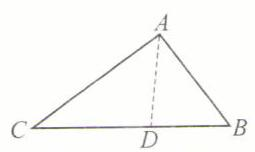
\includegraphics[width=0.2\textwidth]{bodyxb/src/bo_d20cdrf7aajc73bfmvhg_22_565_1962_255_152_0.jpg}
\end{center}


[第 234(1)题]

\begin{center}
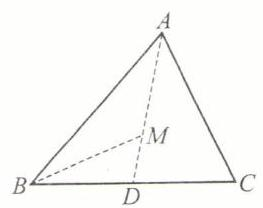
\includegraphics[width=0.2\textwidth]{bodyxb/src/bo_d20cdrf7aajc73bfmvhg_22_902_1901_263_208_0.jpg}
\end{center}


[第 234(2)题]

(2)内心是三角形三条角平分线的交点. 设 $\angle {BAC}$ 的平分线交 ${BC}$ 于点 $D$ . 运用角平分线的性质,如图(2),在 $\bigtriangleup {BAC}$

中, $\dfrac{\left| BD\right| }{\left| DC\right| } = \dfrac{\left| AB\right| }{\left| AC\right| } = \dfrac{c}{b},\;\therefore \;\vv{BD} = \dfrac{c}{b}\vv{DC},\;\therefore \;{AD}$ 的坐标为 $\left( {\dfrac{{x}_{2} + \dfrac{c}{b}{x}_{3}}{1 + \dfrac{c}{b}},\dfrac{{y}_{2} + \dfrac{c}{b}{y}_{3}}{1 + \dfrac{c}{b}}}\right)$ ,

即 $D\left( {\dfrac{b{x}_{2} + c{x}_{3}}{b + c},\dfrac{b{y}_{2} + c{y}_{3}}{b + c}}\right) .\angle {ABC}$ 的平分线交 ${AD}$ 于点 $M$ ,则 $\dfrac{\left| AM\right| }{\left| MD\right| } = \dfrac{\left| BA\right| }{\left| BD\right| },\left| {BD}\right|  = \dfrac{c}{b + c} \cdot  \left| {BC}\right|  = \dfrac{ac}{b + c}$ ,

$\therefore \dfrac{\left| AM\right| }{\left| MD\right| } = \dfrac{b + c}{a},\vv{AM} = \dfrac{b + c}{a}\vv{MD}.\;\therefore$ 点 $M$ 的坐标为 $M\left( {\dfrac{{x}_{1} + \dfrac{b + c}{a},\dfrac{b{x}_{2} + c{x}_{3}}{b + c}}{1 + \dfrac{b + c}{a}},\dfrac{{y}_{1} + \dfrac{b + c}{a},\dfrac{b{y}_{2} + c{y}_{3}}{b + c}}{1 + \dfrac{b + c}{a}}}\right)$ ,即 $M\left( {\dfrac{a{x}_{1} + b{x}_{2} + c{x}_{3}}{a + b + c},\dfrac{a{y}_{1} + b{y}_{2} + c{y}_{3}}{a + b + c}}\right) .$
